\documentclass[a4paper]{article}



%Packages included
\usepackage{graphicx}
\usepackage{multicol}
\usepackage{prettyref}
\usepackage{textcomp}
\usepackage{hyperref}

\usepackage[headings]{fullpage}
\usepackage{fancyhdr}
\usepackage{float}
\usepackage{caption}
\usepackage{amsmath}
\usepackage{subcaption}
\usepackage{cleveref}

\usepackage{todonotes}
\usepackage[
backend=bibtex,
citestyle=authoryear,
sorting=none
]{biblatex}
\addbibresource{../bibliography/refrencedpapers.bib}
\captionsetup[subfigure]{justification=justified,singlelinecheck=false,margin={-0.1cm,0cm}}
%set graphics path
\graphicspath{{../plotting/figures/}}

%opening
\title{The Effect of Bathymetry Changes on Meridional Overturning Currents}
\author{Marte Voorneveld\\
		5911591}


\pagestyle{fancy}
\fancyhead{}
\fancyfoot{}
\fancyhead[C]{\textit{The Effect of Bathymetry Changes on Meridional Overturning Currents}}
\fancyhead[L]{\thepage}
\renewcommand{\headrulewidth}{0pt}

\begin{document}

\maketitle
\noindent\rule{\textwidth}{1pt}
\begin{abstract}
We investigate the effect of changing geometries in a simple ocean general circulation model. Using highly idealized forcings we compare the the situations for every 5 Milion year (Ma) time step from 65Ma to the present day situation. The present day simulation was used as a control. The model result shows a reversal of the flow through the panama gateway in the early Miocene coinciding with the closure of the Thetys seaway. We also observe a system that is extemely senstive to the position of the Indian Continent in the Paleocene. Furthermore we observe large differences in the thermohaline circulations in comparison to the present day situation.
\end{abstract}
\noindent\rule{\textwidth}{1pt}
\begin{multicols}{2}

\section{Introduction}
The geometry and resulting bathymetry of our planet is an ever changing phenomenon. In the last 120 Ma the earth moved from having one major oceanic system in the Pacific with a single large continent to the current 3 ocean system (\cite{besse2002apparent}). The Bathymetry changes that occurred in this time period are characterized by the opening and closing of certain passages through which exchange of water between the oceanic basins is observed. The exact timing of passage openings is a topic of rigorous debate in literature (\cite{Scher2006Apr}, \cite{Schmidt2007Jan}).


One of the changes on which there is general consensus, is the inception and expansion of the Atlantic ocean and the resulting decrease in size of the Pacific basin. The creation of the Atlantic basin has had major effects on the earth's climate, especially resulting in massive localized changes such as the temperate European climate, due to the north Atlantic meridional overturning current (AMOC). This creates the current Northern sinking oceanic throughflow in the Atlantic. However it is unknown when exactly this northern sinking started. With the past non-existance of the Atlantic it must have started some time in the last 40Ma with the advent of a larger Atlantic (\cite{Abelson2017onset}). 

The result of these bathymetry changes on the oceanic stream function and the resulting overturning currents is something that has been previously studied by \cite{Mulder2017Jul}. They however found that using a Jacobian matrix for continuation in each of the model years fails to simulate the onset of the Northern sinking AMOC that is physically observed. Here we instead propose to use a general circulation ocean model with only a changing bathymetry keeping the same initial forcing for each time step. This eliminates the need for a continuation using the Jacobian matrix method proposed in \cite{Mulder2017Jul}.

This paper will focus solely on changes in bathymetry using simplified zonally averaged global forcings. The results of the model will be used to estimate global changes in oceanic through flow at the critical passages. Furthermore the strength of the meridional overturning currents (MOC) will be studied.


\section{Methods}

%TODO (ON THE THERMOHALINE CIRCULATION)
\subsection{Veros and Runtime}
Ocean modeling has been an area of continued progress. The resolutions of the models have been steadily increasing since the inception of the first computerized ocean models. However, due to the age of some of these models and the continued adaptation of often old legacy Fortran code, many models have become enormous hurdles to get started with often resulting in frustration. The Veros ocean model project is trying to tackle this problem with a totally new code base written entirely in Python (\cite{Hafner2018Aug}). 
Veros is a General Circulation Ocean model based on the successful PyOm2 model. It was designed from the ground up with flexibility in mind. This flexibility cuts valuable time spent on figuring out the often cumbersome Fortran models of the past. Veros is specifically well suited for researching the effect of changes in both forcings and bathymetrys. They can be easily edited using Python. These features in particular are heavily used in this paper. One of the most extensively used features for example is the fact that any bathymetry can, without further manual specifications of islands be used for stream function calculation.

In this case the models used in this paper are run on a 8 core (16 threads) machine using an MPI CPU configuration of 1 node.



\subsection{Model Setup}
\subsubsection{Model Domain}
The domain of the model is bounded by longitudes $\phi_E=-180^{\circ}$ and $\phi_W=-180^{\circ}$ and latitudes $\theta_N=80^{\circ}$ and $\theta_S=-80^{\circ}$ with periodic boundary conditions in the zonal direction.
Furthermore the model uses restoring boundary conditions. Restoring the boundary at the surface of the oceanic basin to be a value based of a forcing field for Sea Surface Temperature (SST), Sea Surface Salinity (SSS), wind stresses ($\tau$) and heat flux.
 The depth profile has 15 layers with grid stretching (\cref{fig:gridstrech}). The grid stretching relation is such that surface layers are much shallower than deep water layers. There are $90 \times 40$ grid points to make a $4^{\circ} \times 4^{\circ}$ resolution model.
 
 \begin{figure}[H]
 	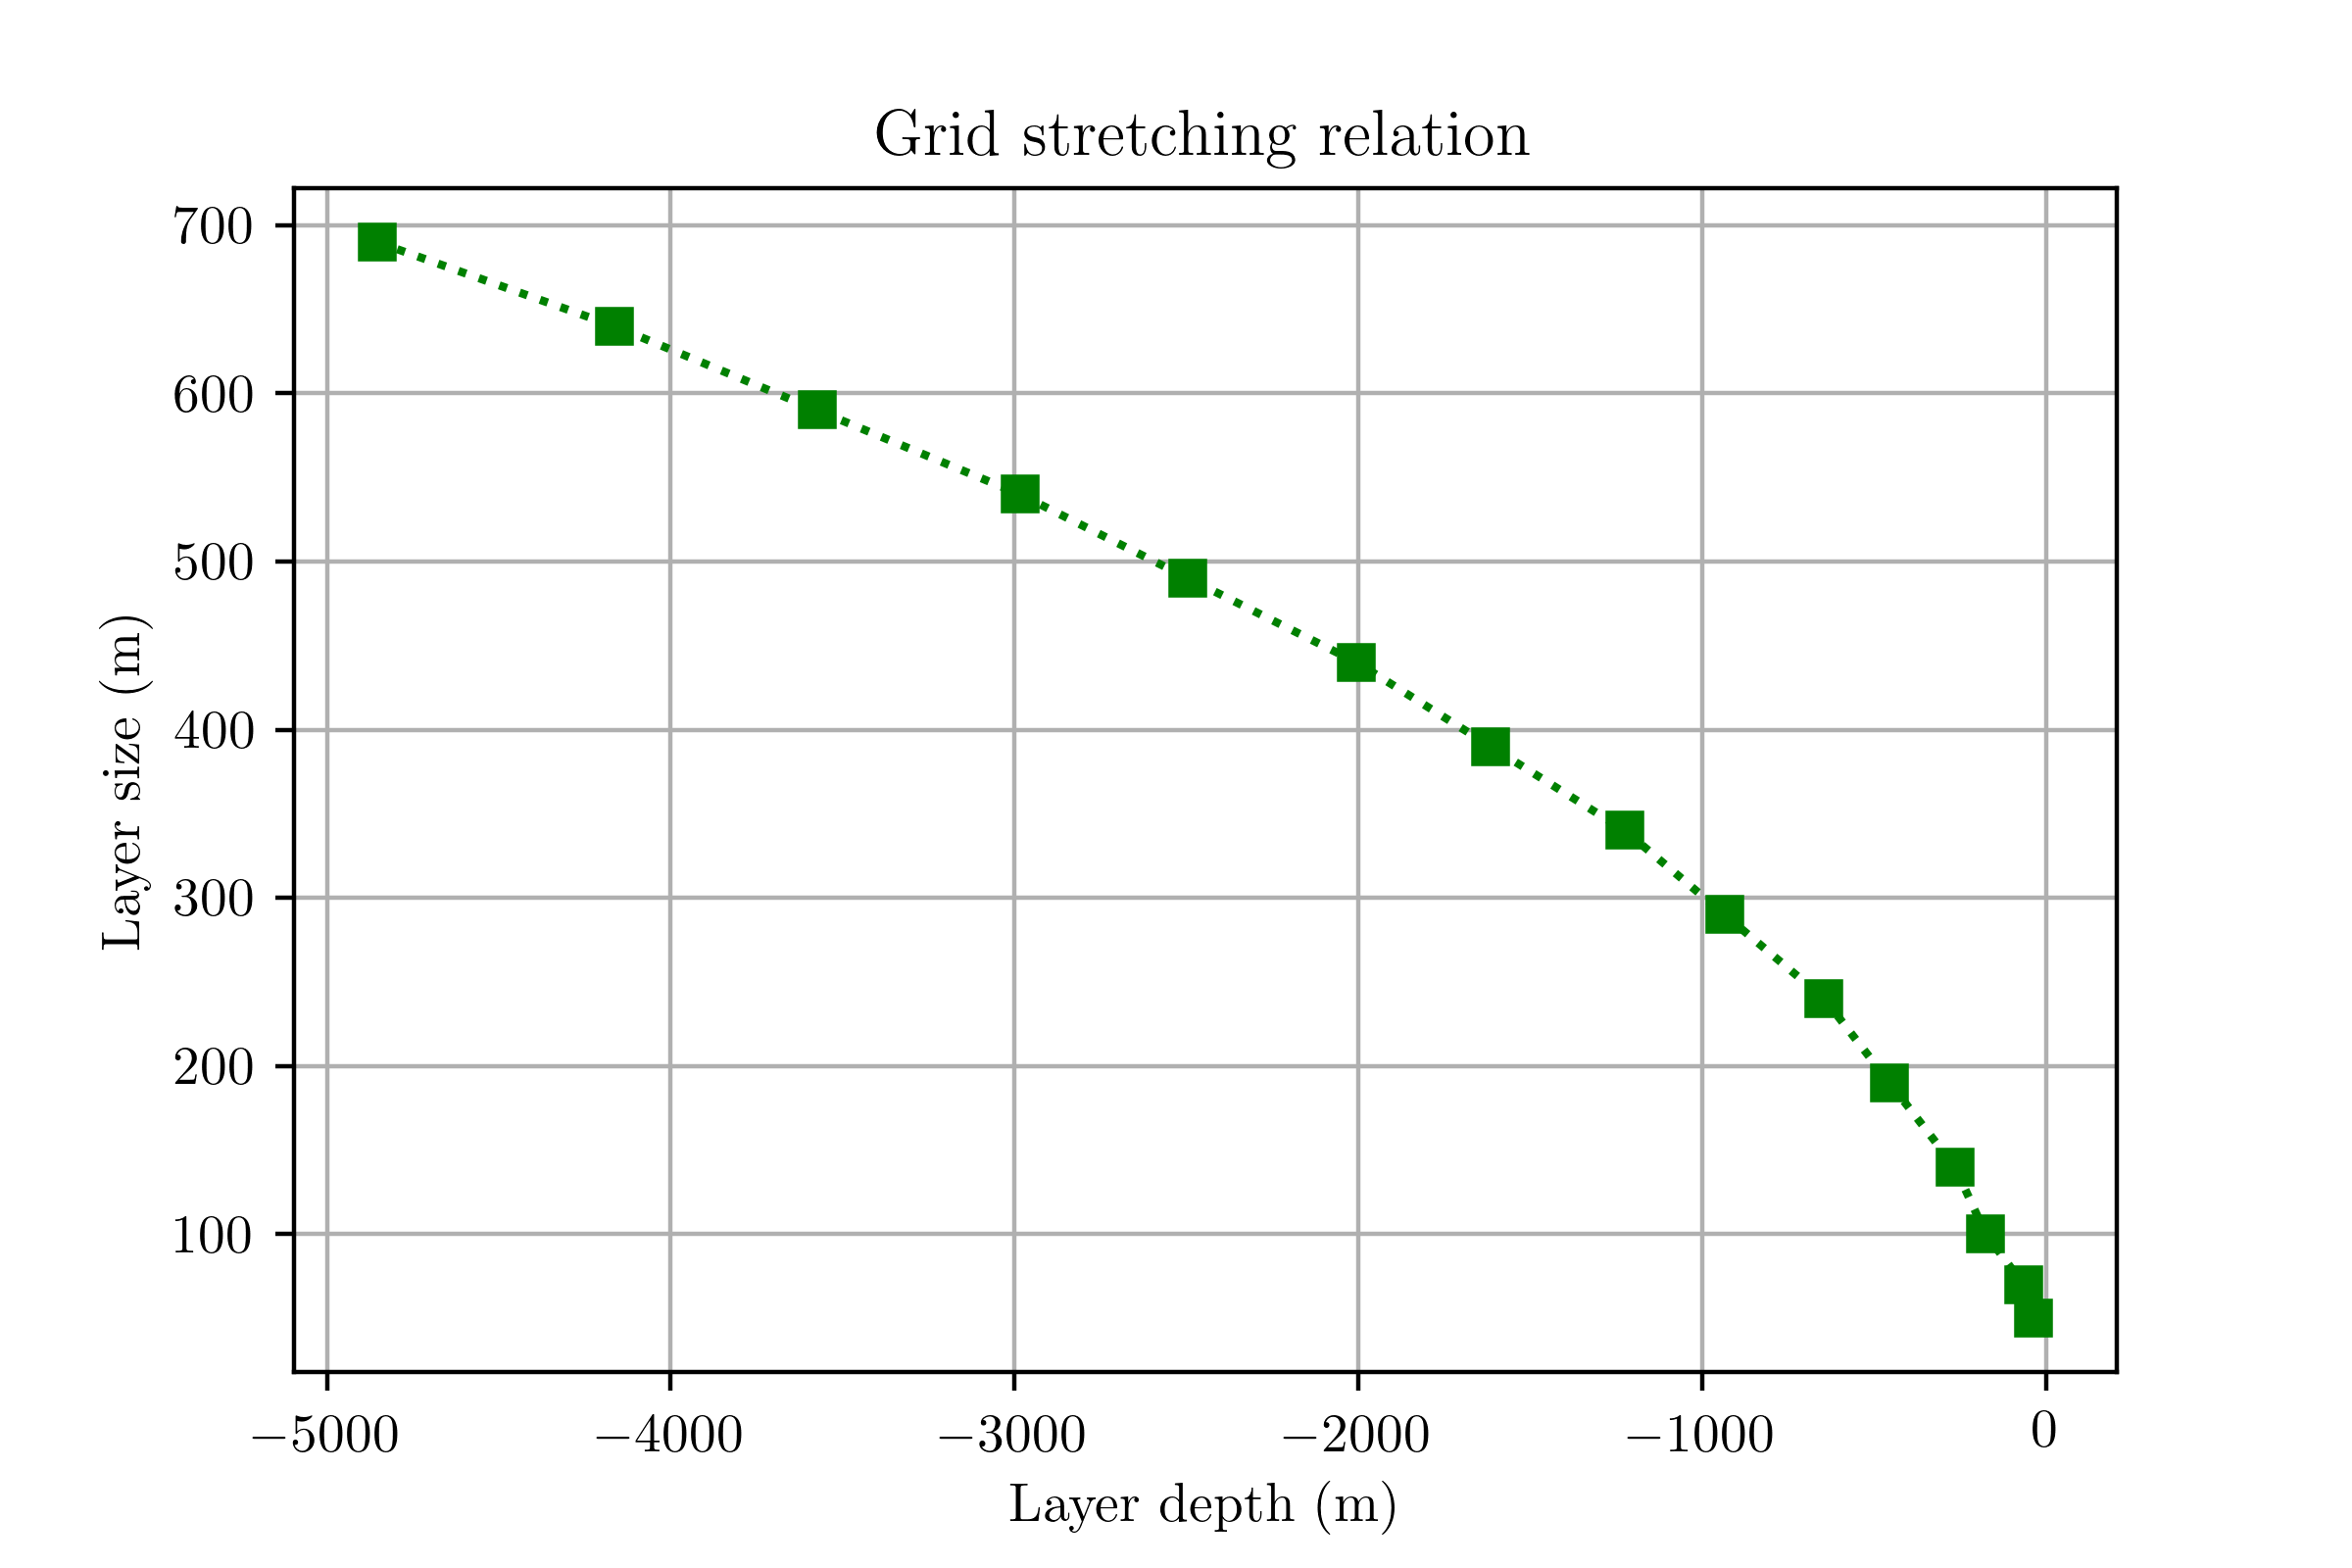
\includegraphics[width=\linewidth]{grid_stretching.png}
 	\caption{Figure of the grid stretching relation used.}
 	\label{fig:gridstrech}
 \end{figure}

\subsubsection{Surface Forcings}
 Choosing the correct forcing for the ocean is very important. It is known that in general circulation models the MOC is highly sensitive too even small changes in surface forcings (\cite{Milliff1999May}). Attempts at making these forcings highly idealized have often been made in the past with varying rates of success(\cite{bryan1987parameter}; \cite{Mulder2017Jul}). We note the fact that, using idealized forcings will probably induce the errors, especially in the shape of the thermohaline circulations.
 
 There were several methods that are explored when it comes to creating these idealized forcings. In the \cite{Mulder2017Jul} paper an analytic forcing profile was used for wind flux, SST and SSS (\cref{fig:idealized_forc}). Veros is however a seasonally forced model. Using these simplified forcings would thus fail to capture seasonal changes especially in the SST. There have been studies suggesting that these seasonal forcings can have large effects on the strength of the meridional overturning circulation (\cite{schmittner2001seasonally}). Here we propose to take the SSS, SST and heat flux profiles as as zonal means for each month in the earths rotation. While the Zonal wind stress is set to the simple profile proposed by \cite{bryan1987parameter}. The choice of this analytic profile was made over a zonally averaged and equatorial averaged forcing $\mu(\tau_x)$. These were both tested on the present day configuration to see which of these forcings most accurately captures the present day MOC. We find that the Zonally averaged wind stress is very weak in the subpolar regions and fails to force the north Atlantic deep water formation discussed in \cref{sec:MOCSTREAM}.
\end{multicols}
%example full width overturning

\begin{figure}[H]
\begin{subfigure}{.5\textwidth}
	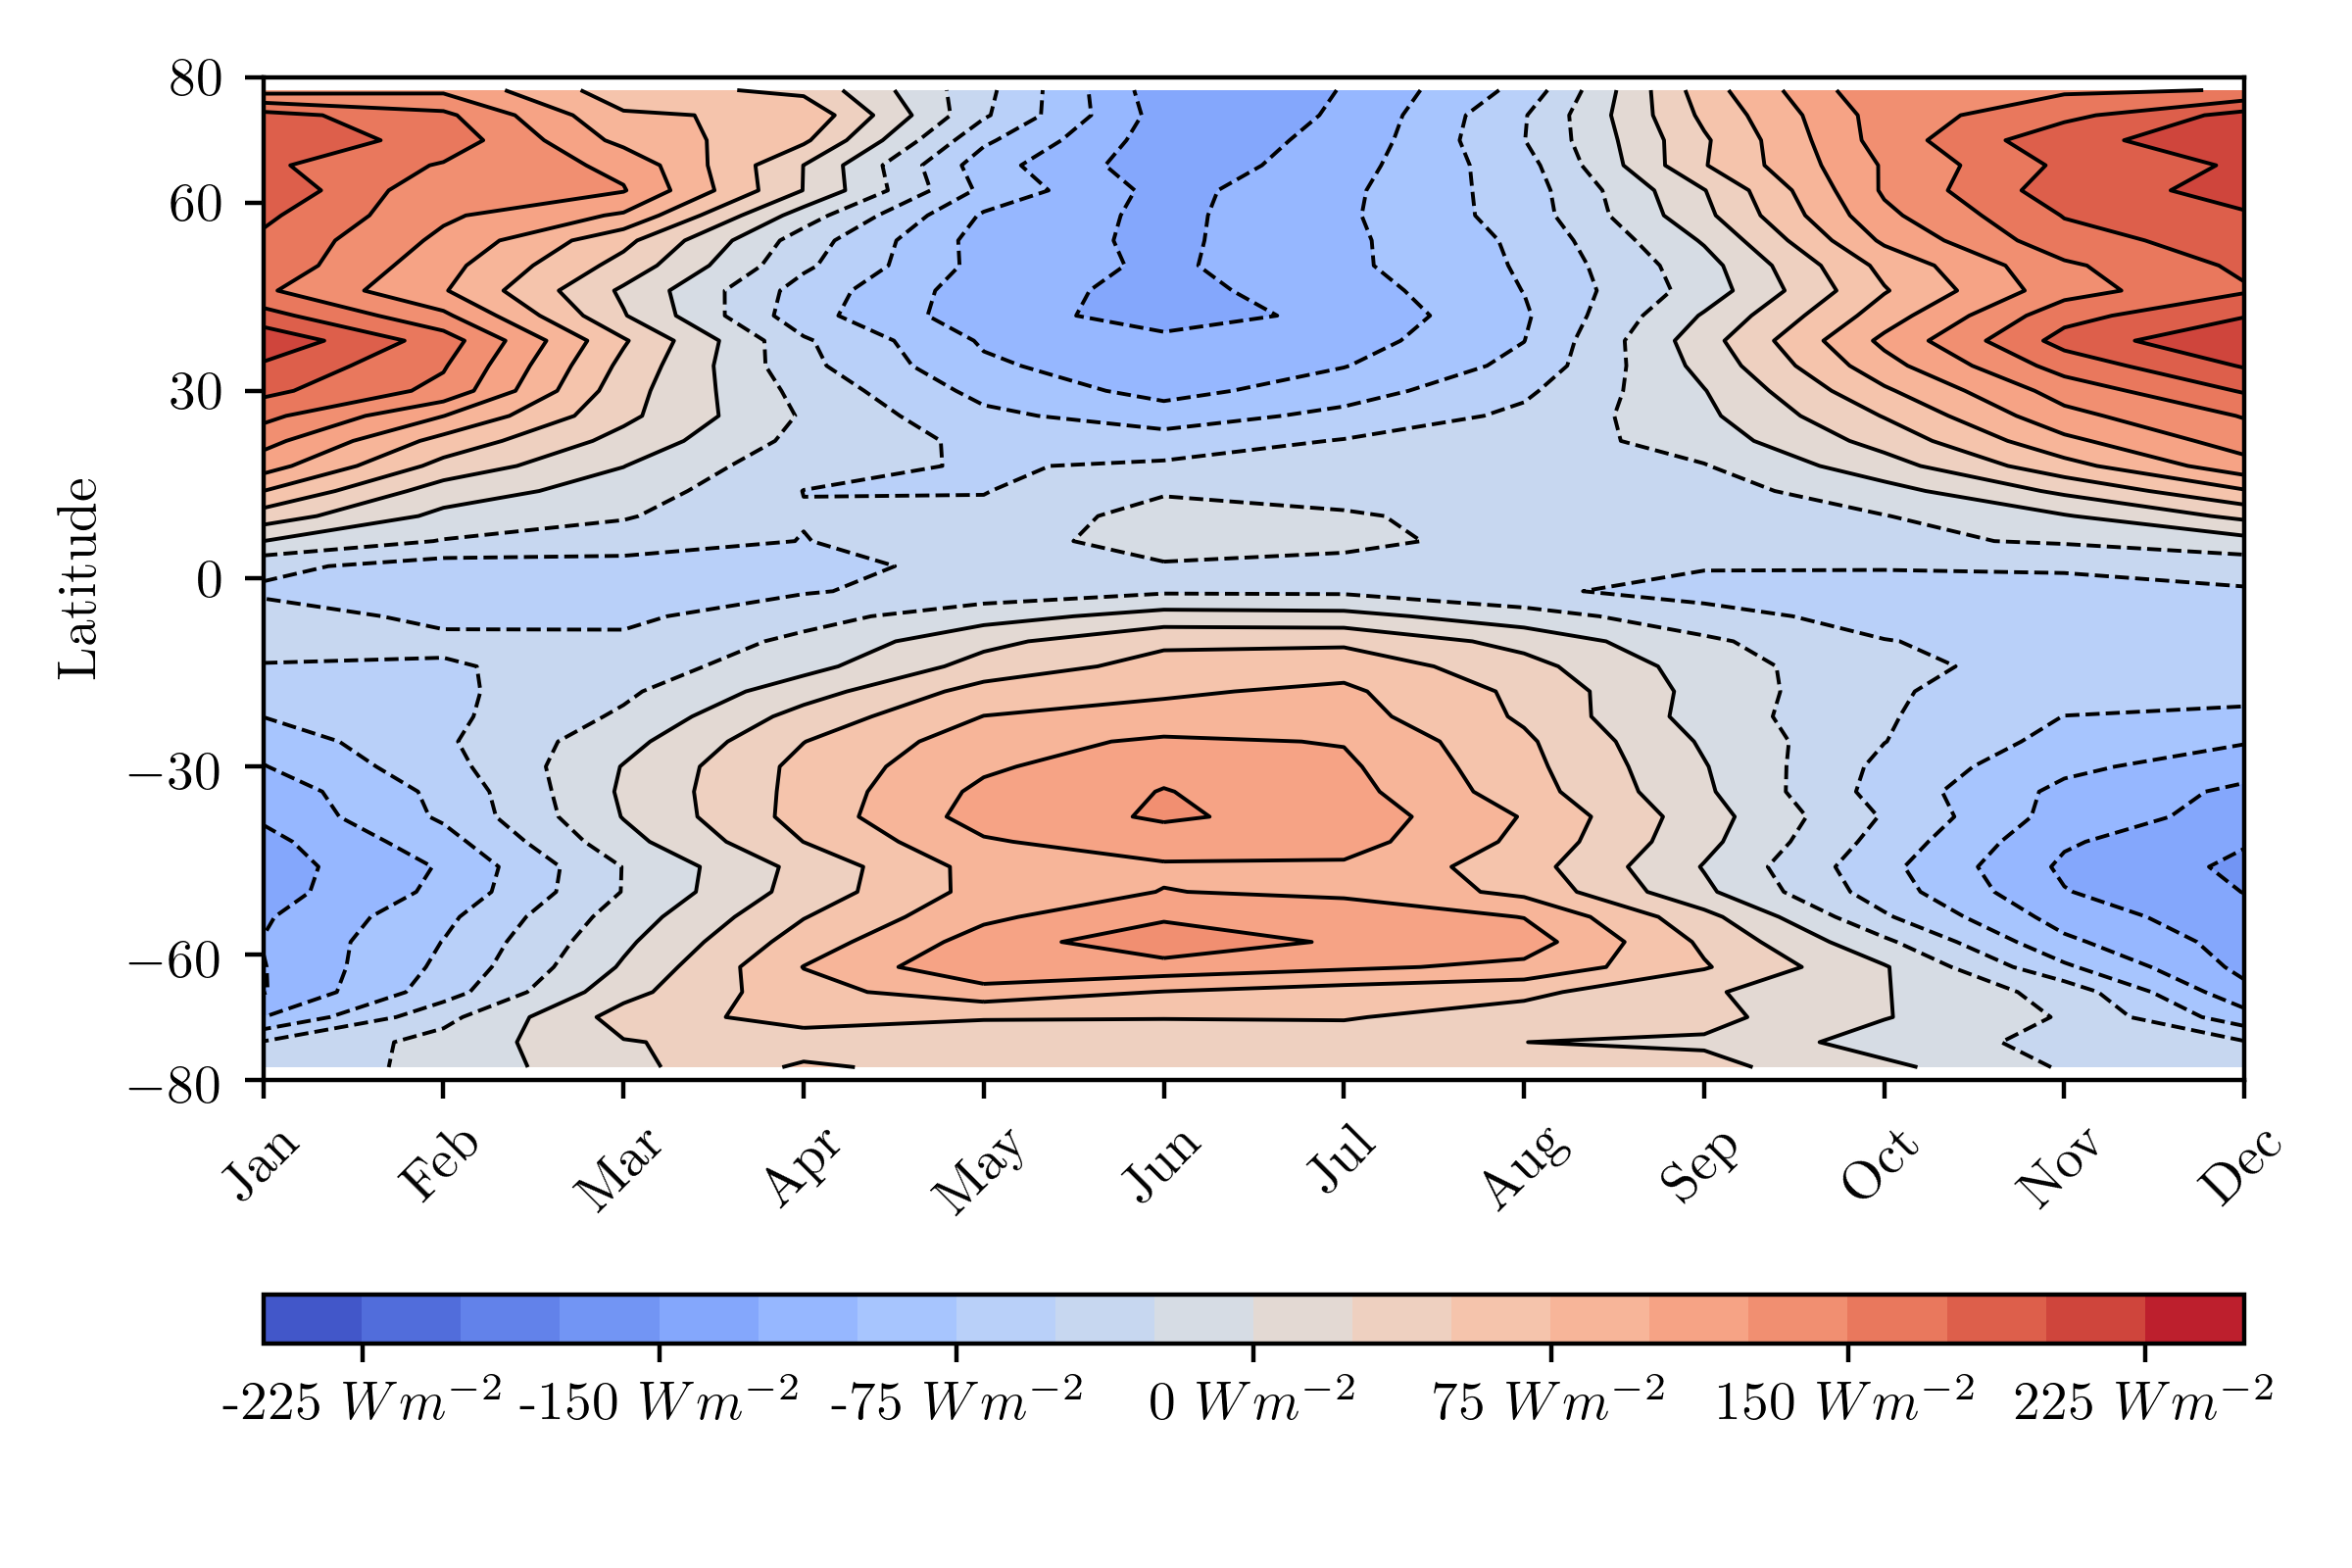
\includegraphics[width=\linewidth]{q_net_profile.png}
	\caption{Net Heat flux}
	\label{fig:qnet}
\end{subfigure}
\begin{subfigure}{.5\textwidth}
	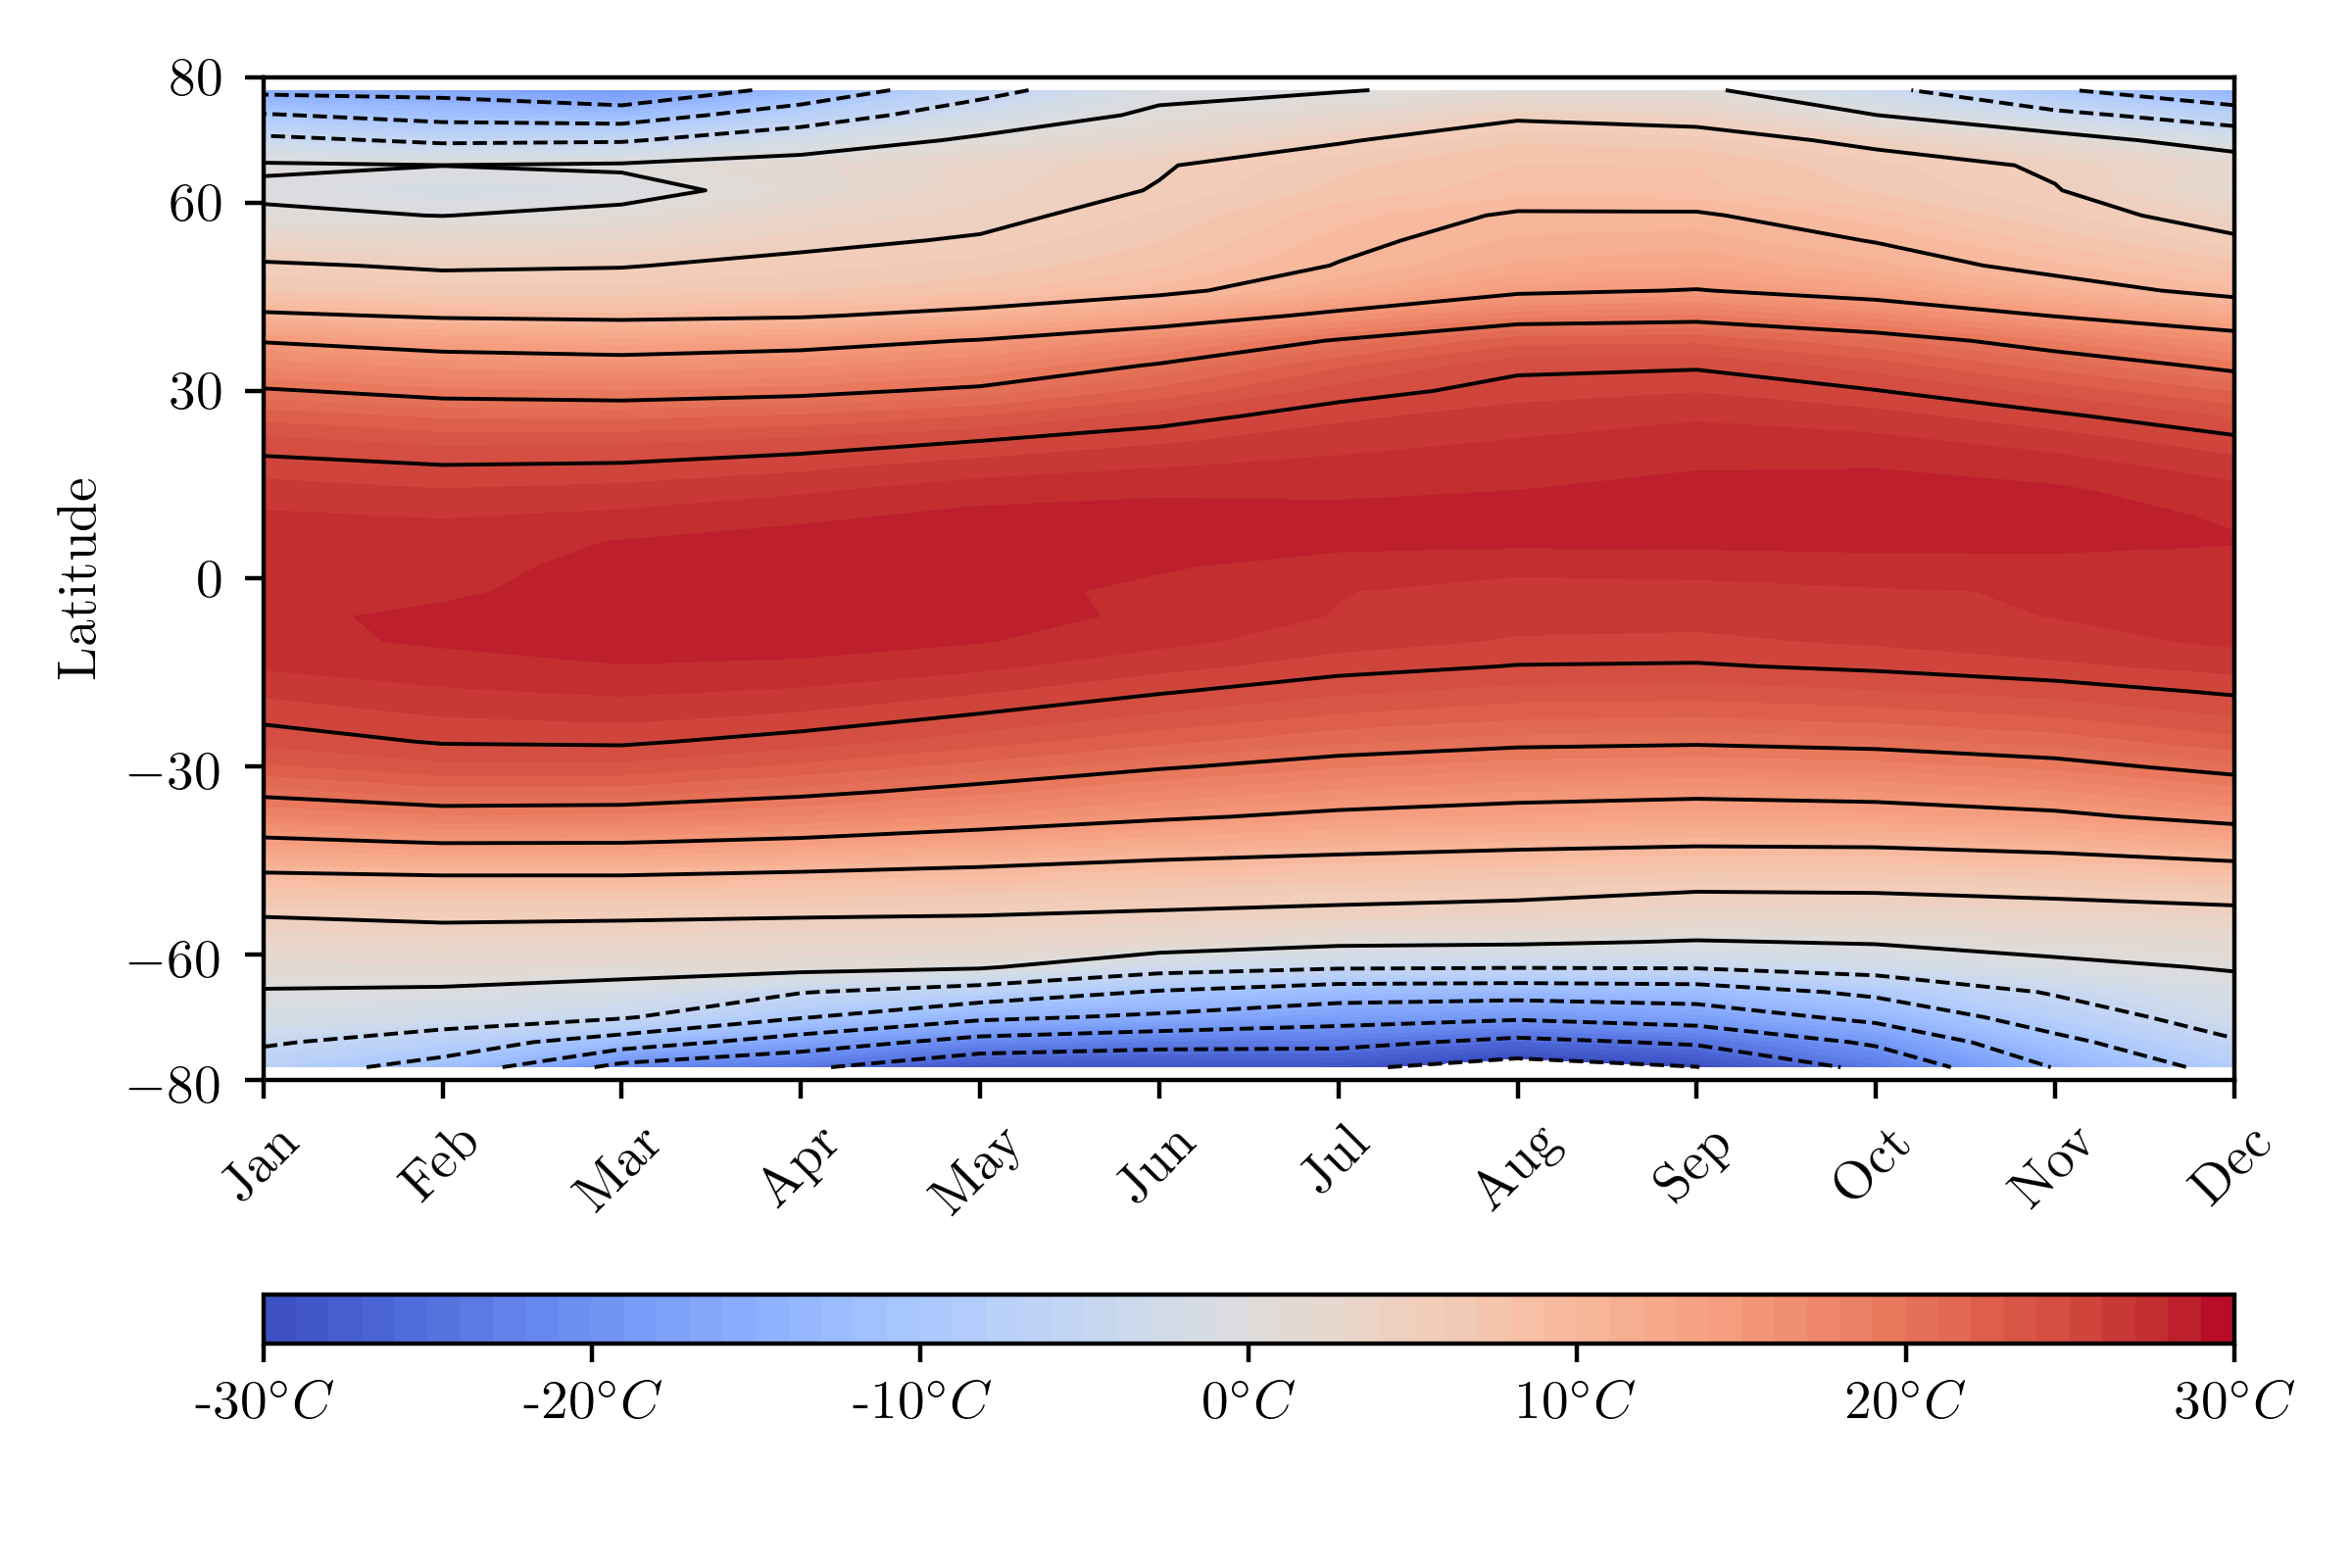
\includegraphics[width=\linewidth]{sst_profile.png}
	\caption{SST profile}
	\label{fig:sst_profile}
\end{subfigure}
\begin{subfigure}{.5\textwidth}
	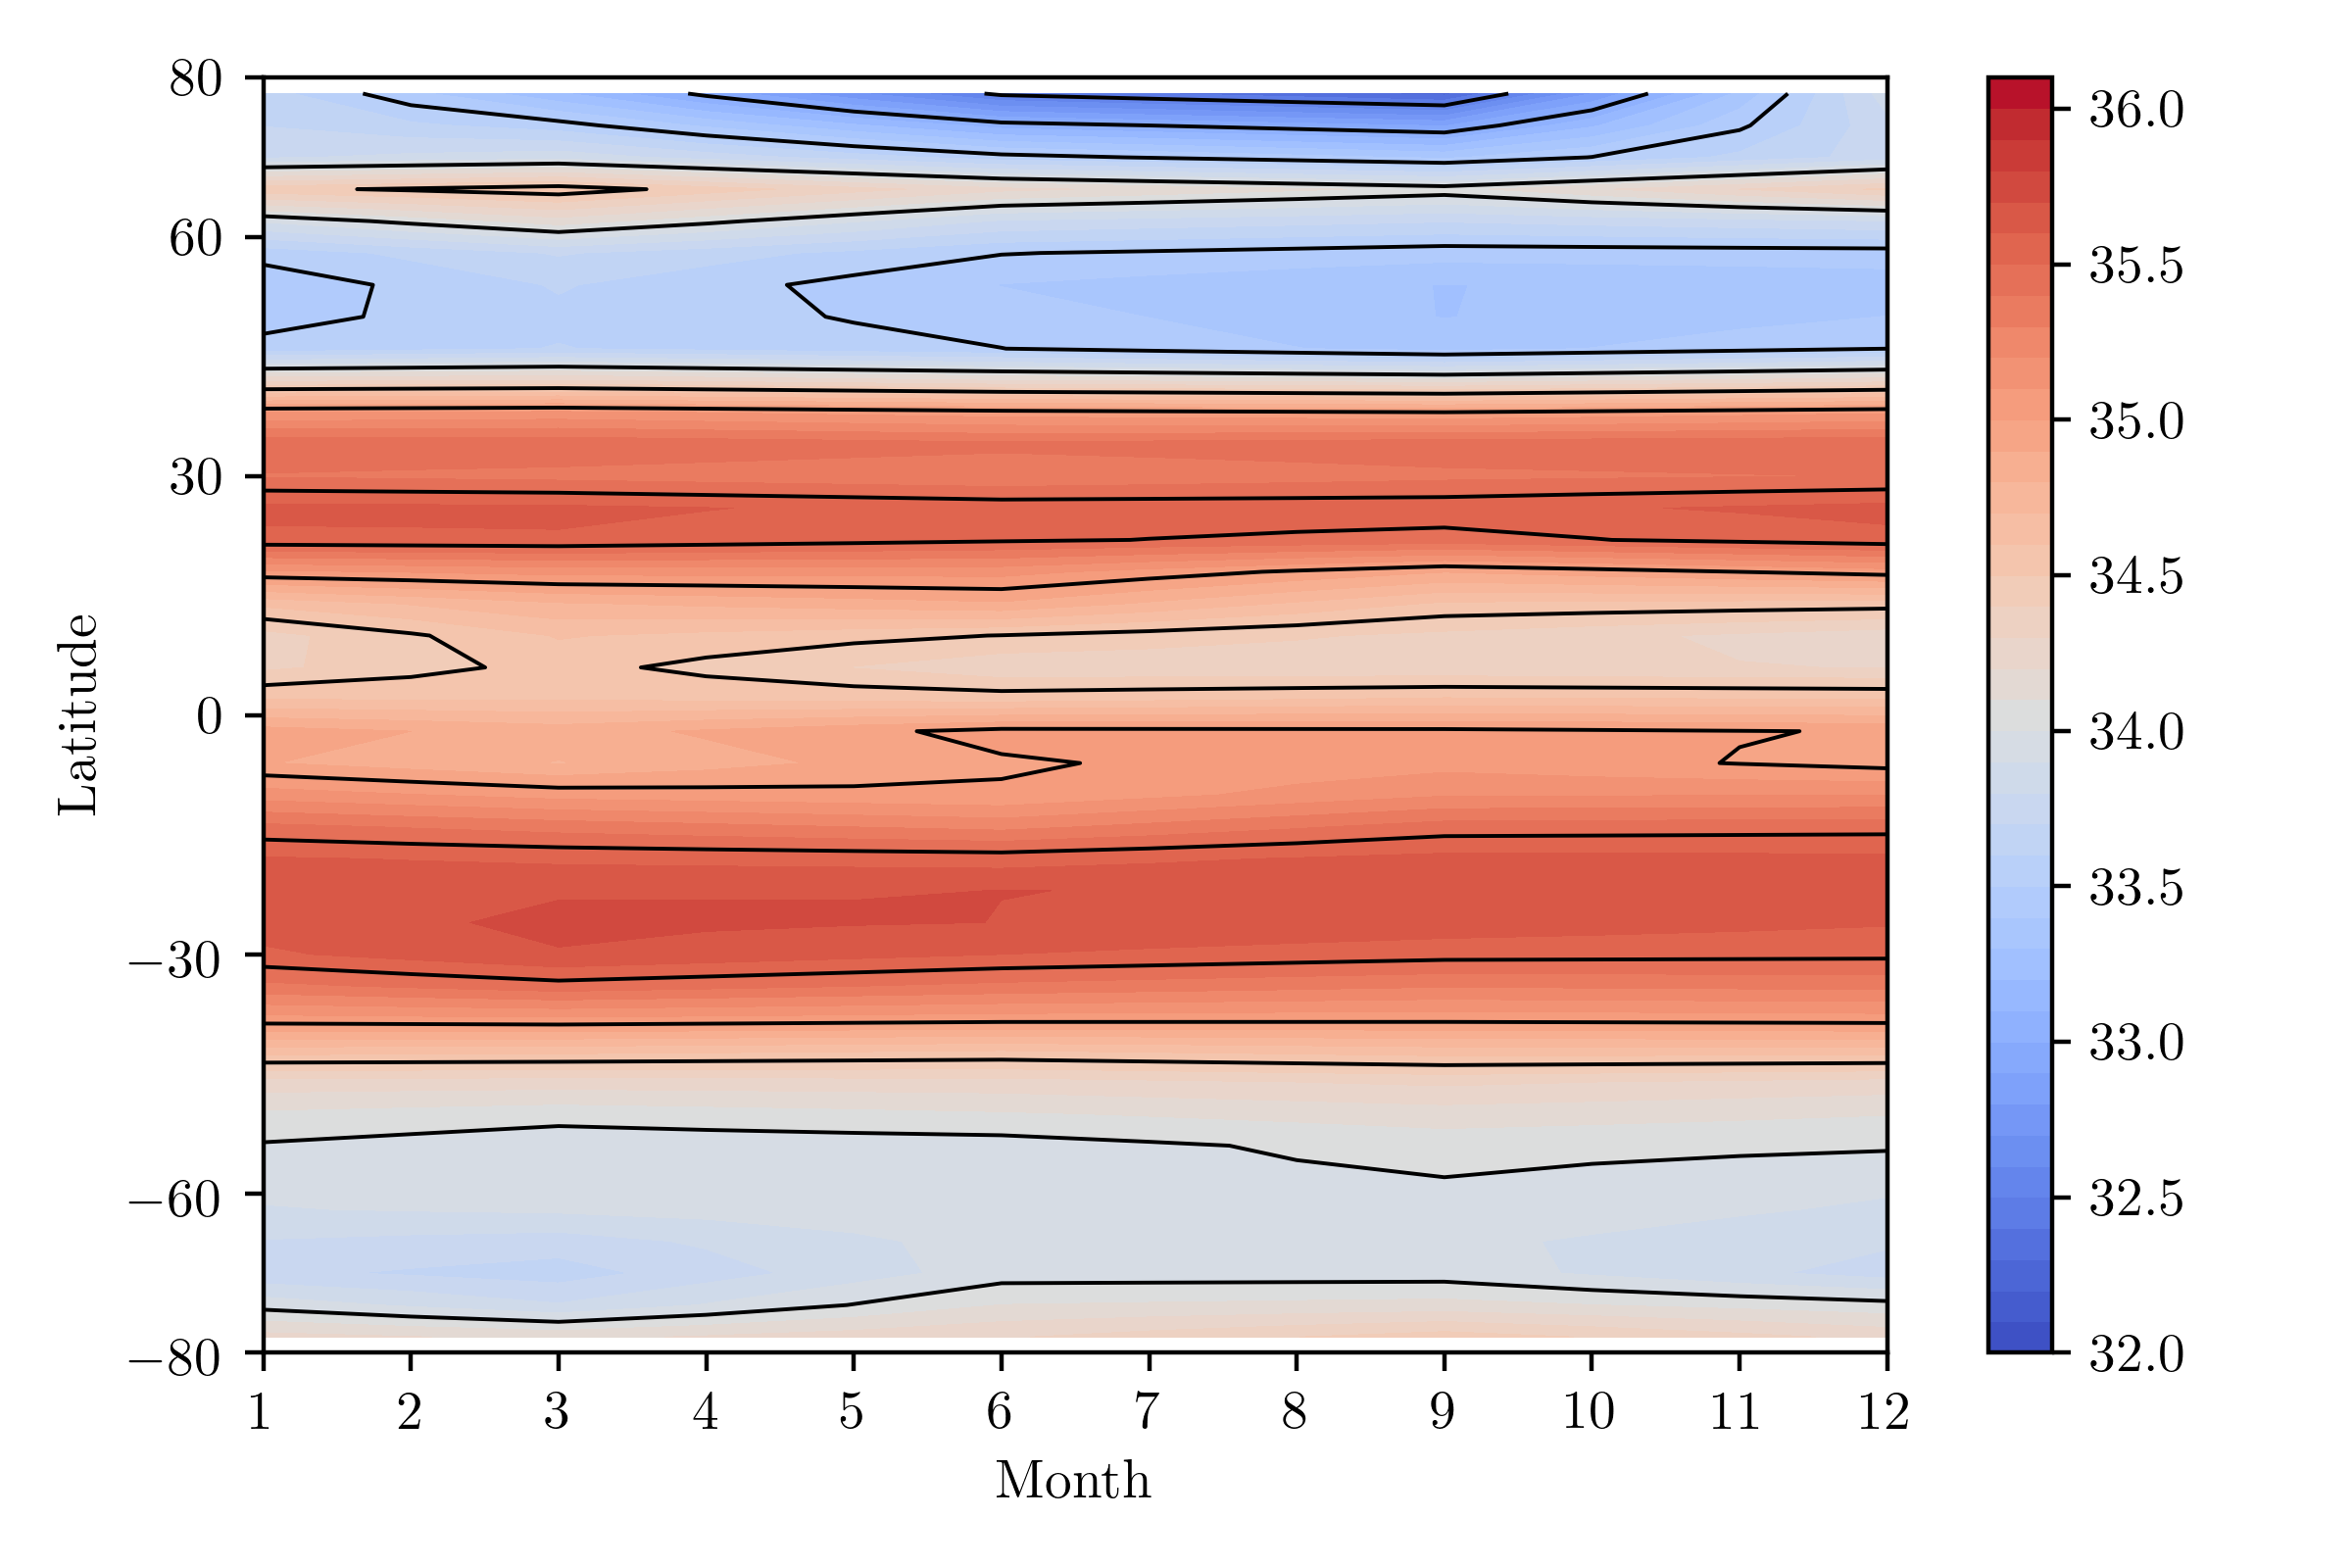
\includegraphics[width=\linewidth]{sss_profile.png}
	\caption{SSS profile}
	\label{fig:sss_profile}
\end{subfigure}
\begin{subfigure}{.5\textwidth}
	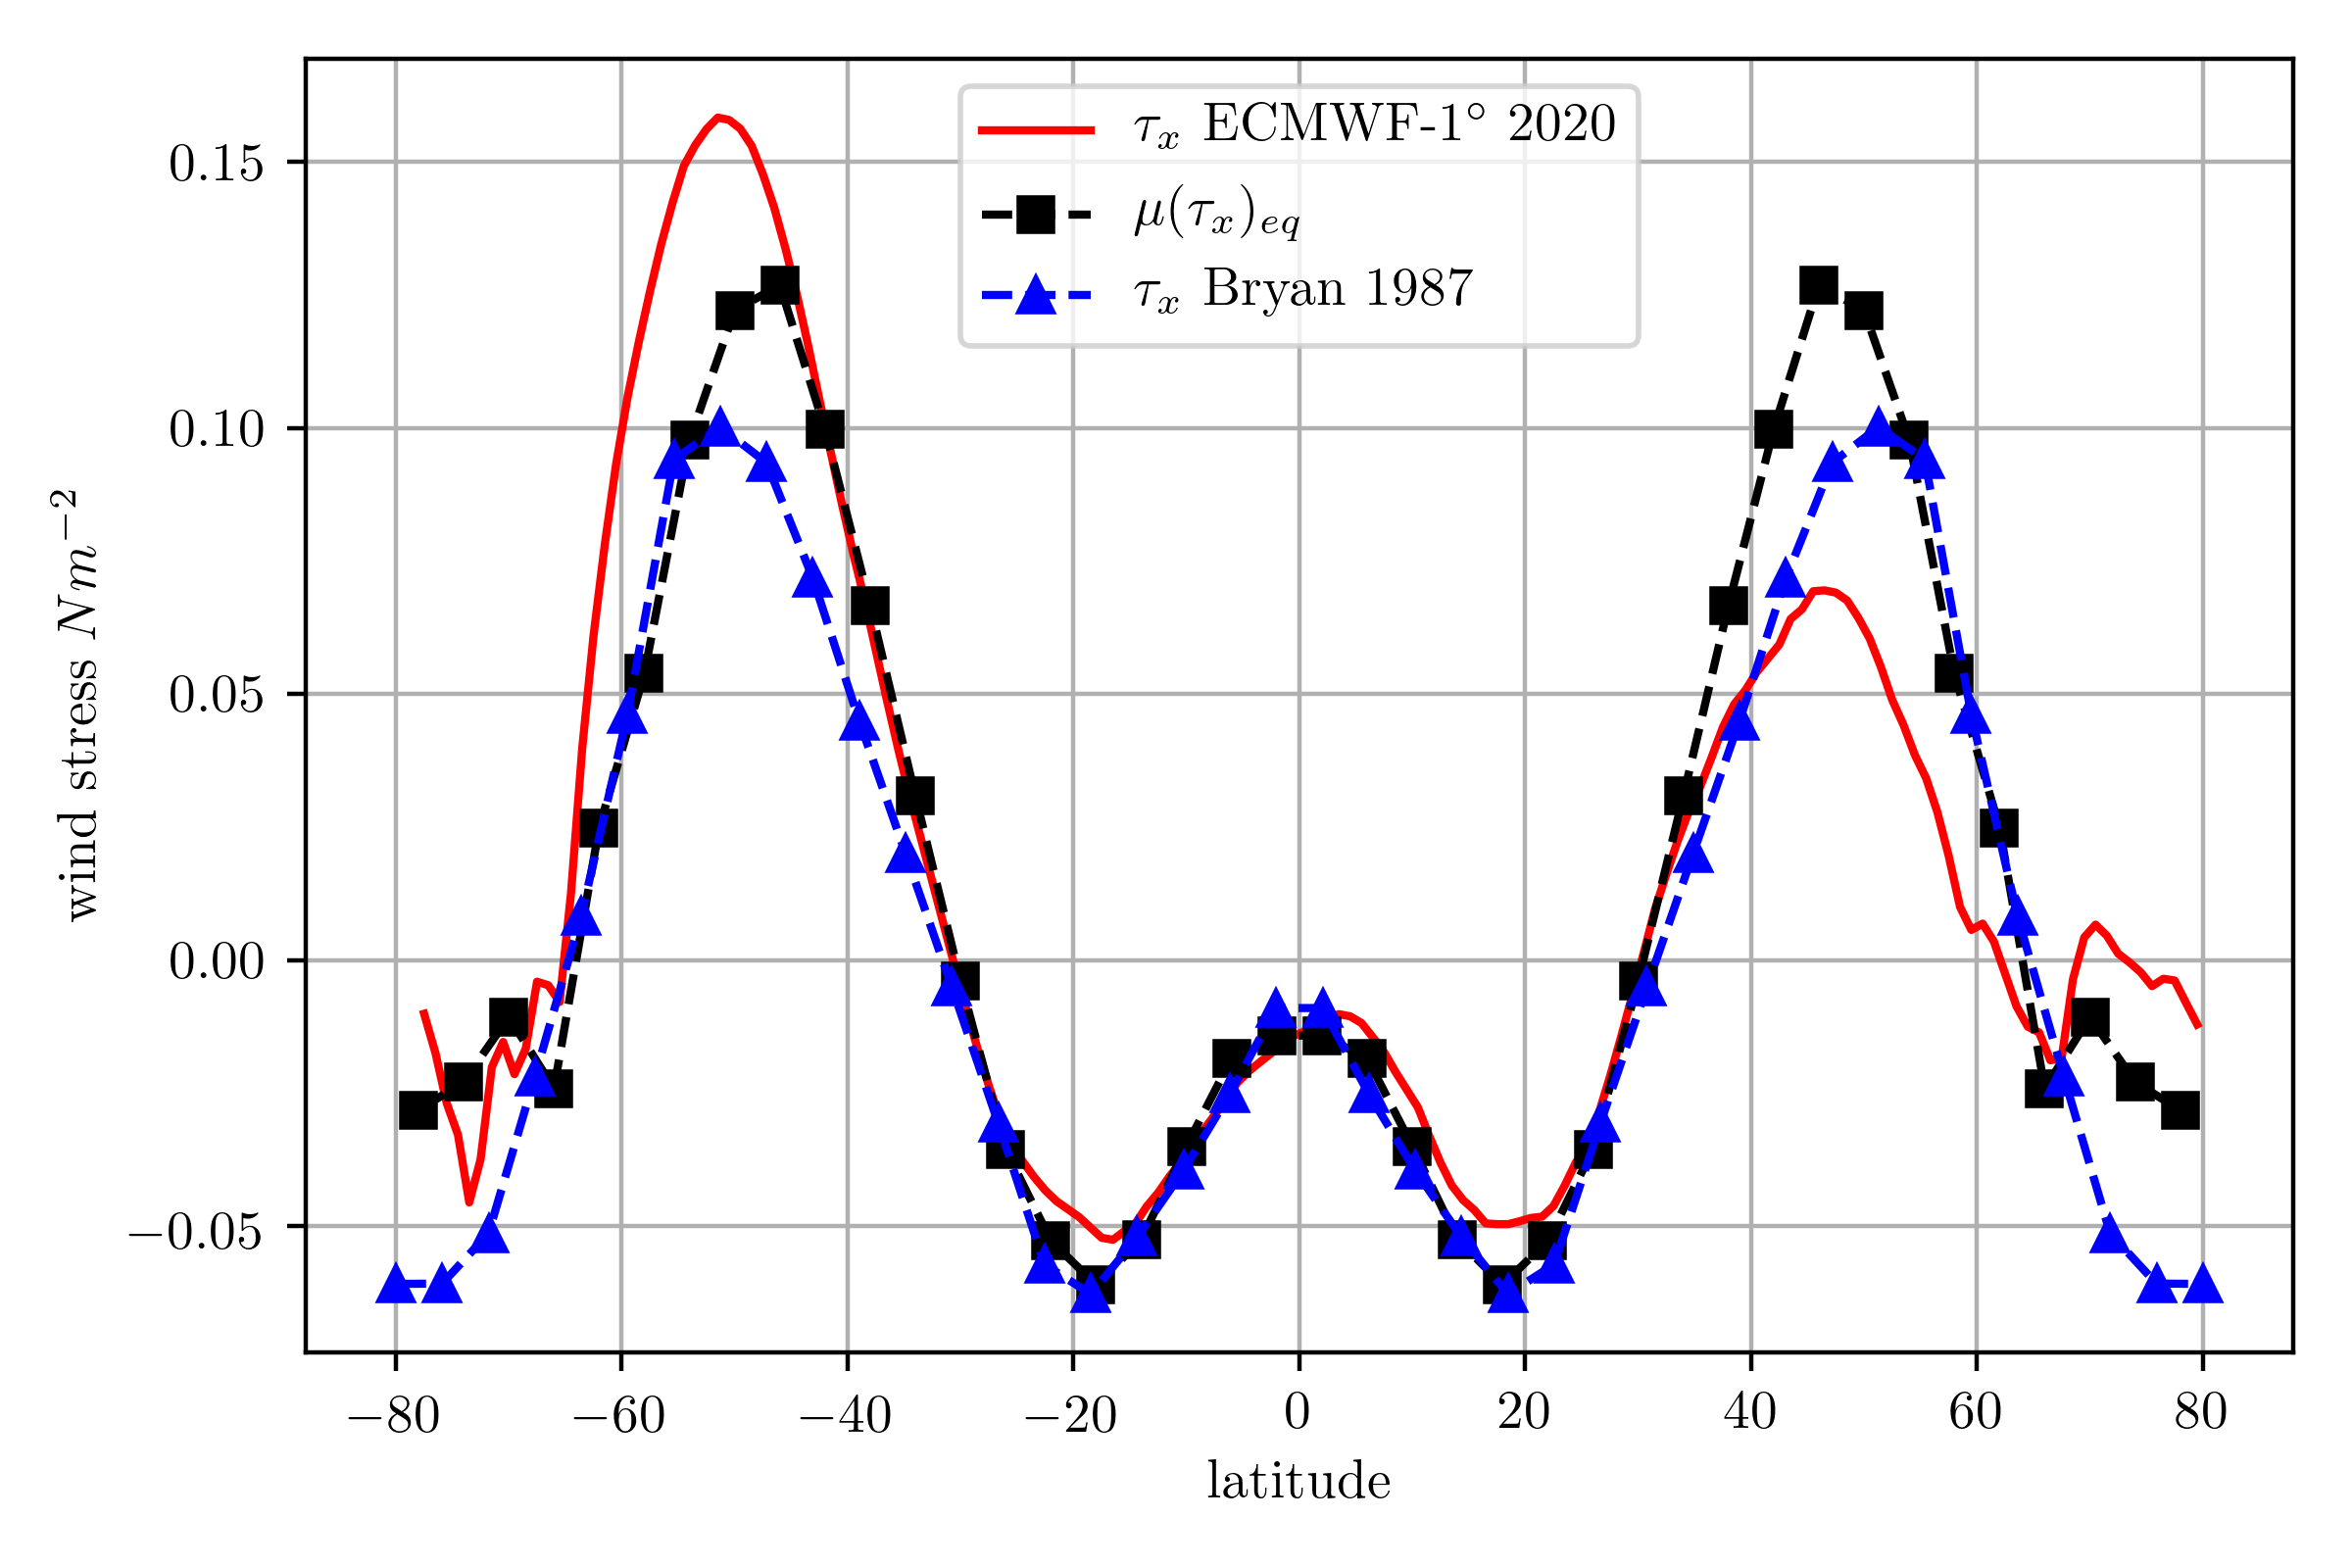
\includegraphics[width=\linewidth]{windstress_models.png}
	\caption{$\tau_x$ profile}
	\label{fig:tau_profile}
\end{subfigure}
%\begin{subfigure}{.5\textwidth}
%	\centering
%	% include first image
%	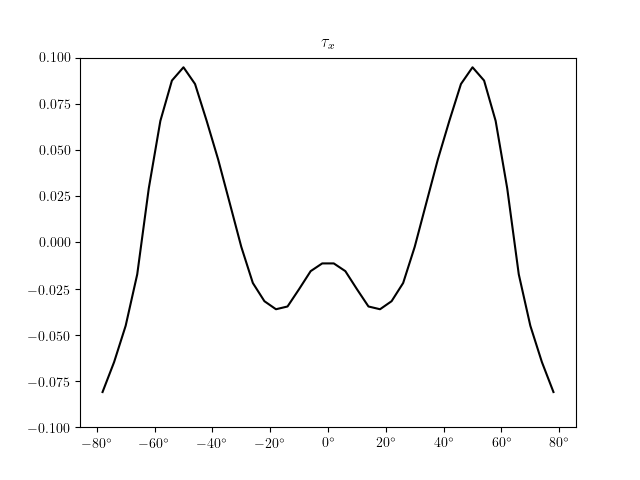
\includegraphics[width=0.9\linewidth]{tau_x_profile.png}
%	\caption{Zonal wind stress ($\tau_x$) profile}
%	\label{fig:tau_X}
%\end{subfigure}

\caption{Idealized forcing profiles}
\label{fig:idealized_forc}
\end{figure}

\begin{multicols}{2}
 \subsubsection{Forcing errors} \label{sec:forc_err}
The forcings we use here have large errors compared to reality. This can be seen if we compare the original realistic forcings to the zonal mean of these forcings. In \cref{fig:sss_sst_errors} there is a particularly large discrepancy in the Atlantic. Which has a much higher salinity in reality than in our forcing. This may have large implications on the thermohaline circulation. It is furthermore noted that the northern Atlantic ocean is much warmer in reality than in our model. Again possibly having an effect on the thermohaline circulation.
\end{multicols}
\begin{figure}[H]
	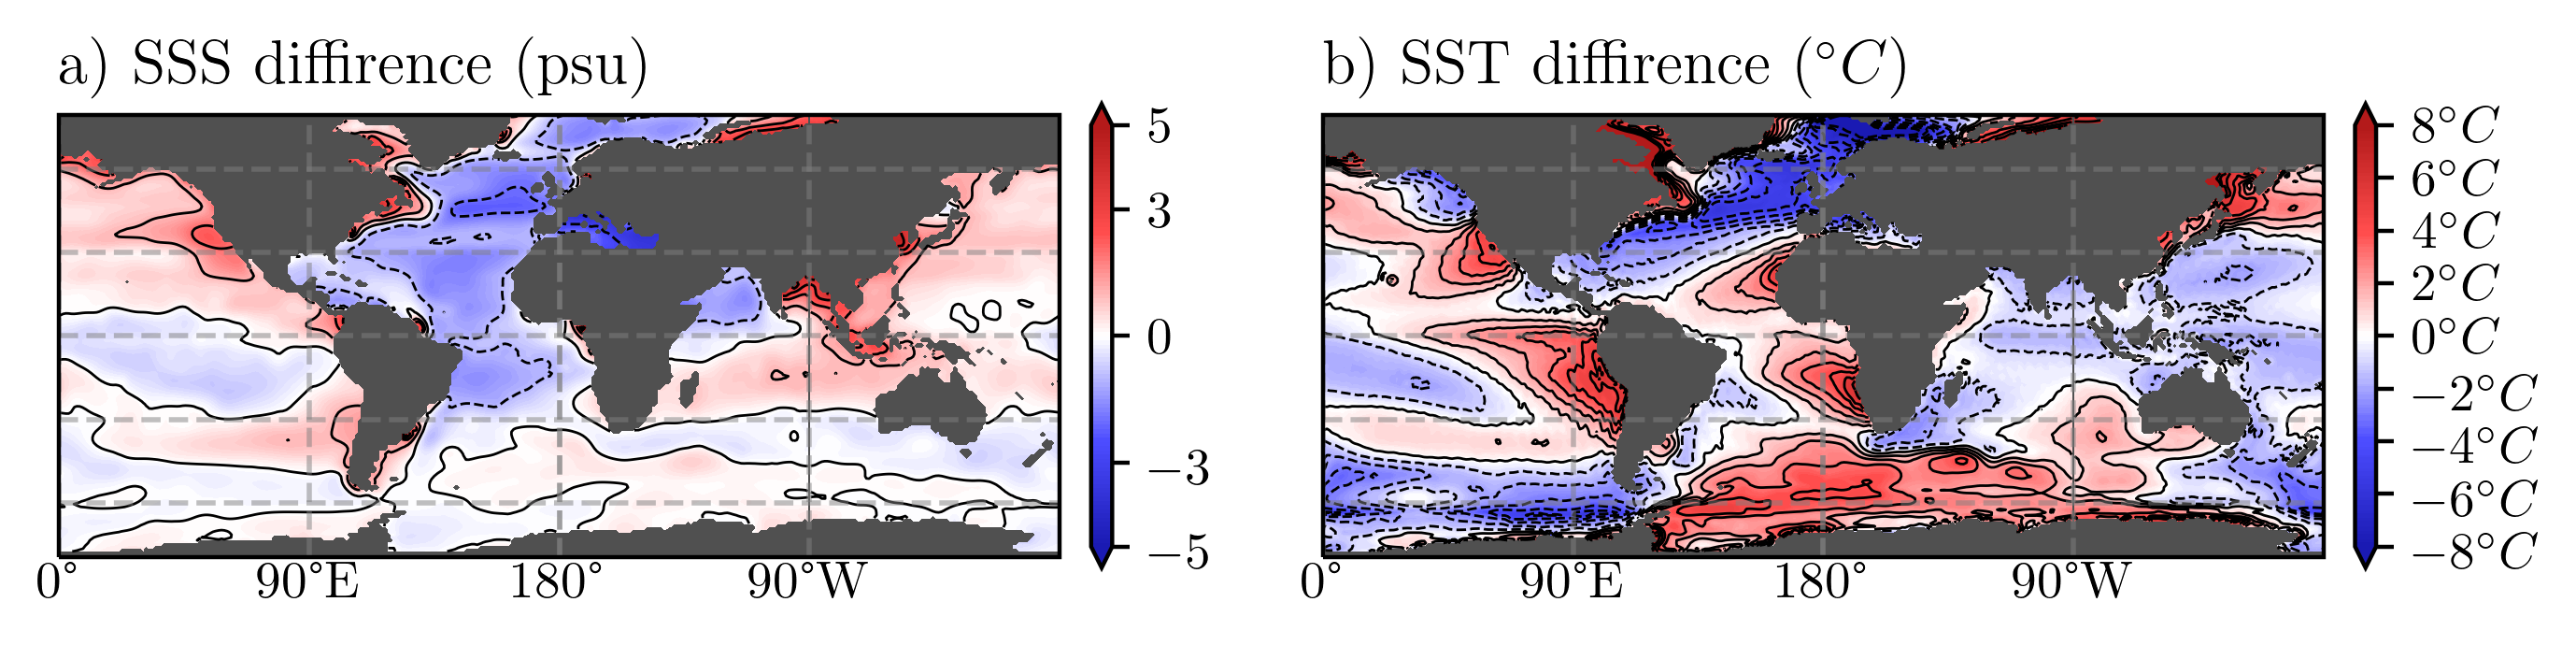
\includegraphics[width=\linewidth]{SST_SSS_errors.png}
	\caption{Figure showing errors in surface forcing. Here positive values are over estimations of realistic forcings. Errors for: \textbf{a)} the SSS difference with contours every 1 psu and \textbf{b)} the SST difference with contours every 1 $^{\circ}C$}
	\label{fig:sss_sst_errors}
\end{figure}
\begin{multicols}{2}
 \subsubsection{Initial conditions}
The model is started with an initial temperature and salinity profile that is, like the forcings taken from observational data. A zonal mean was taken for the profiles. This results in the profile seen for the situation around the equator in \cref{fig:salt_temp_prf}.

\begin{figure}[H]
	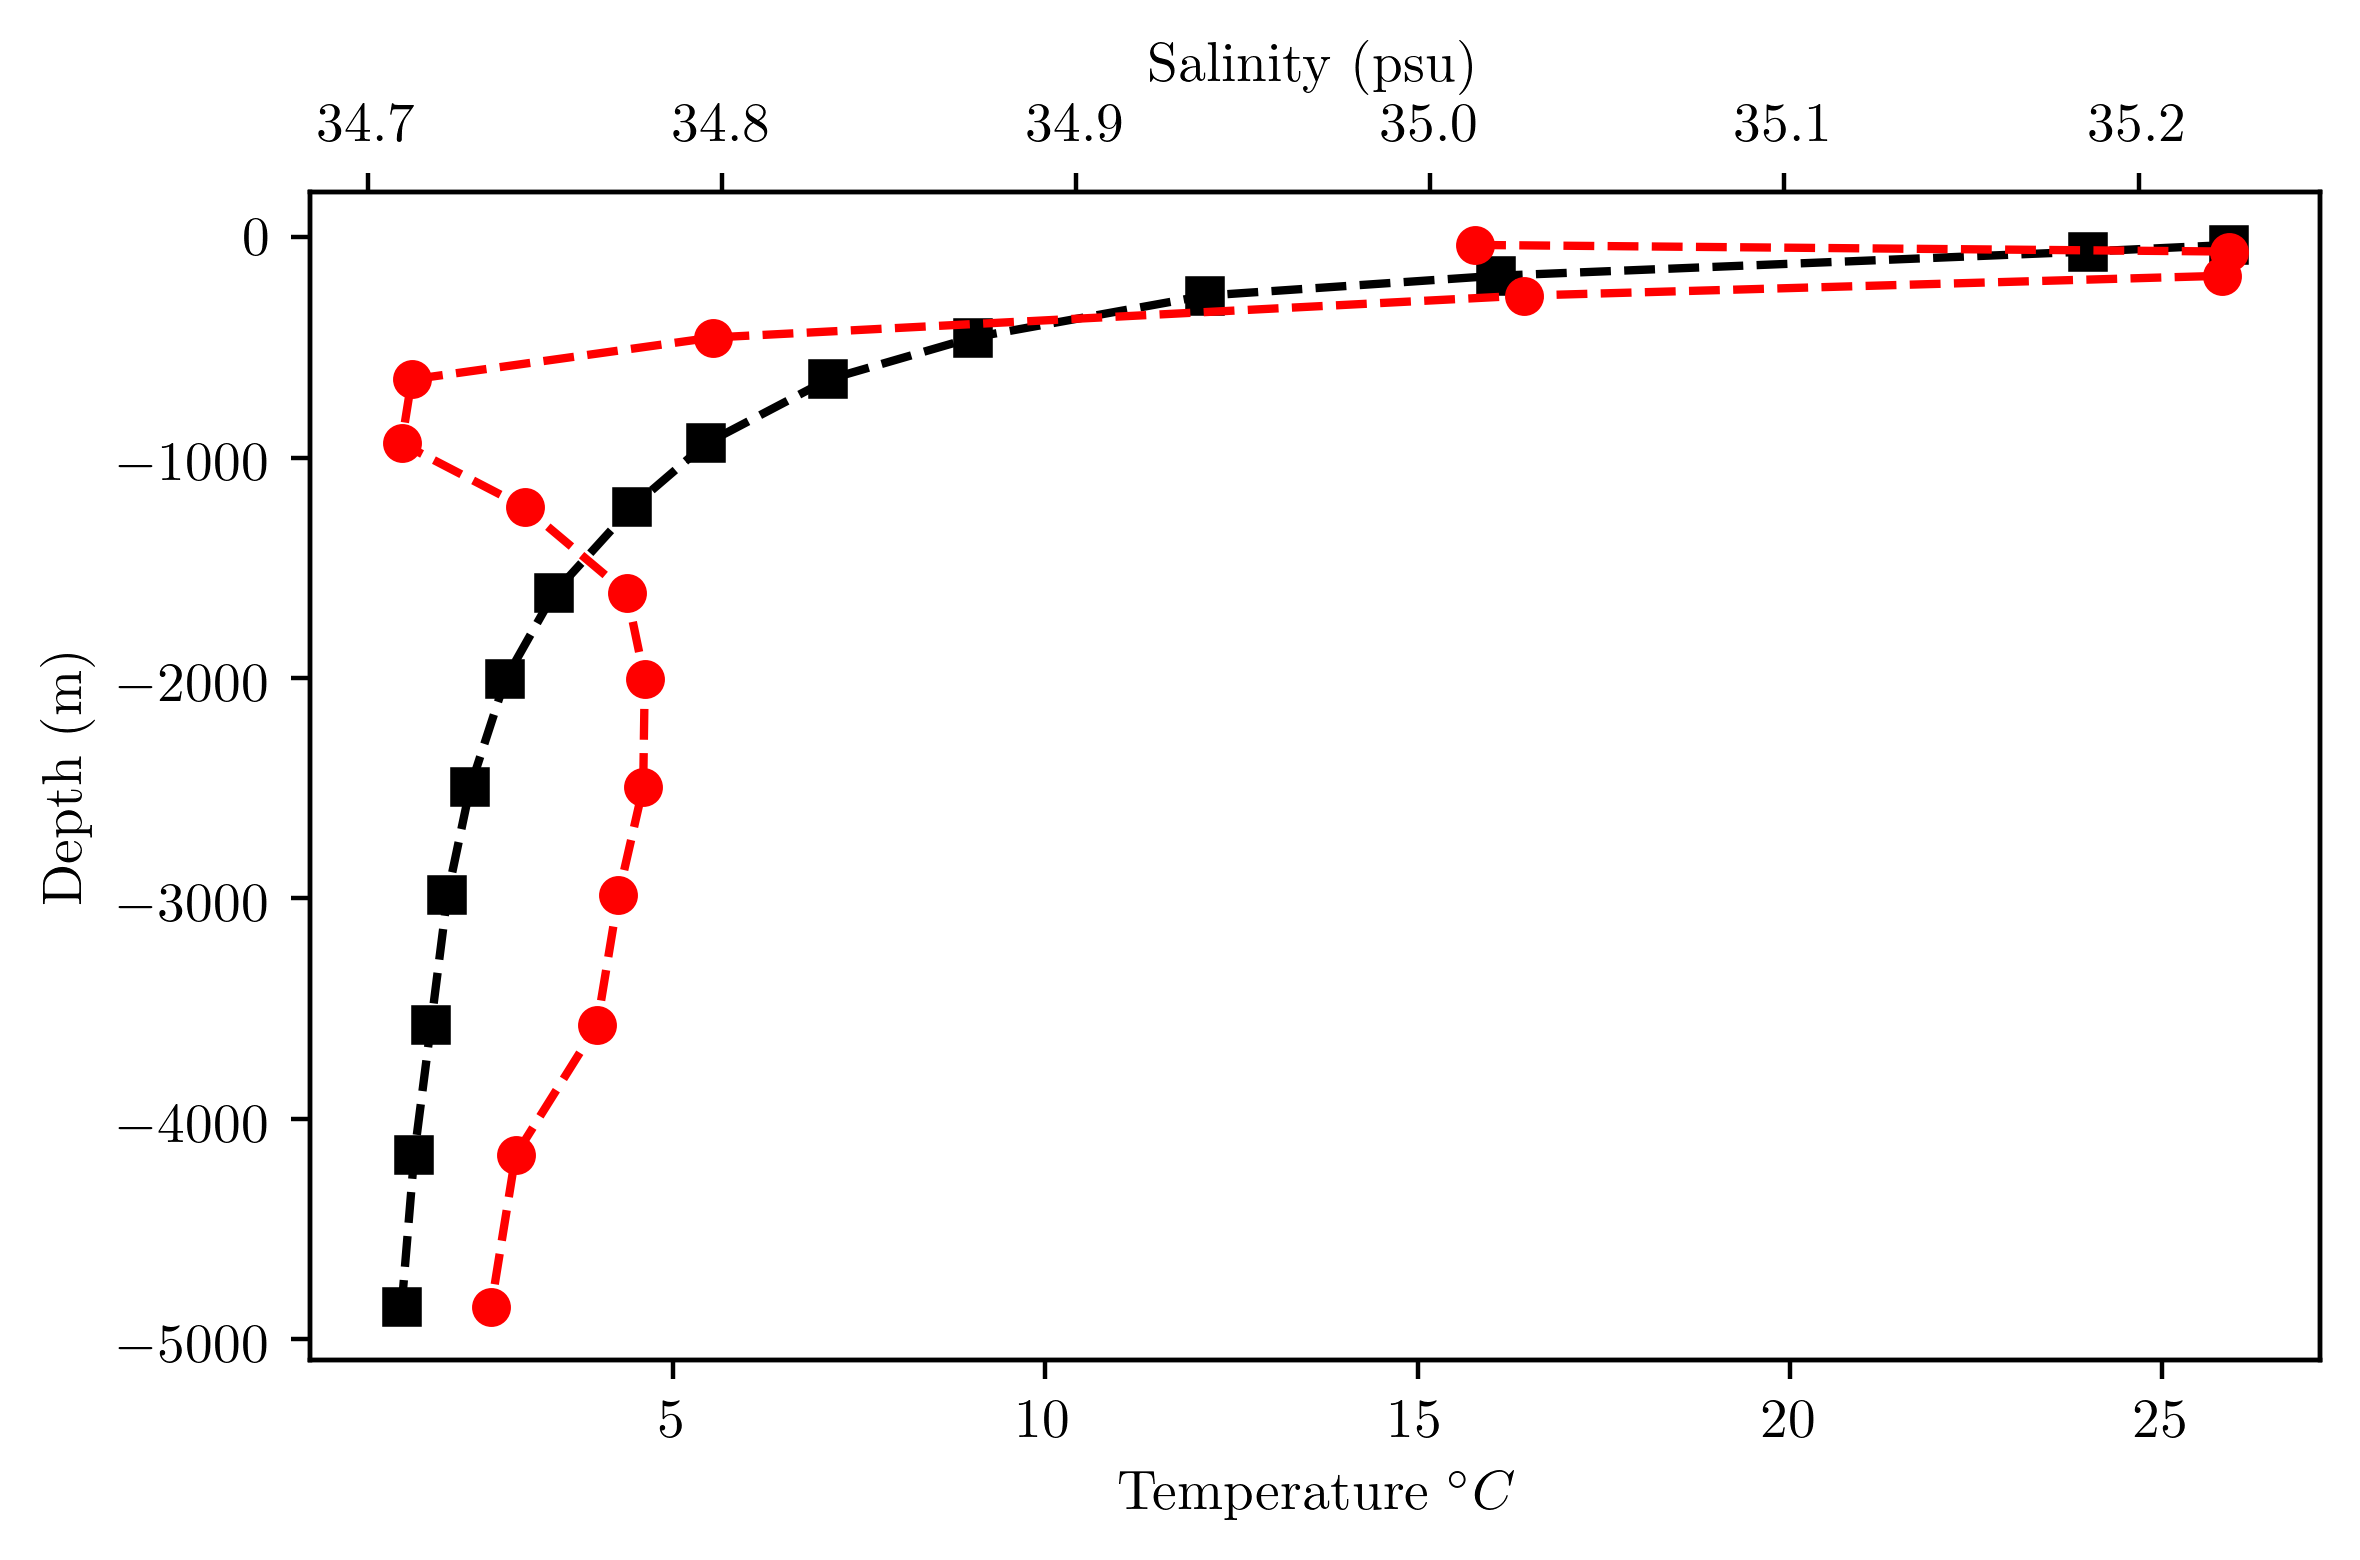
\includegraphics[width=\linewidth]{salt_temp_prof.png}
	\caption{Figure showing the temperature and salinity profiles at $2^{\circ} N$. Black squares indicate the Temperature profile and red circles indicate the salinity profile.}
	\label{fig:salt_temp_prf}
\end{figure}
 
 \subsubsection{MOC stream function} \label{sec:MOCSTREAM}
 
 The global Meridional Overturning Circulation $\Psi_{MOC}$ is defined as the zonally integrated meridional volume transport of water in the worlds oceans. It can be written down as:
 
 $$
 \Psi_{MOC}(y,z) = \int_{z}^{0} \int_{-180^{\circ}}^{180^{\circ}} v(x,y,z') dx dz'
 $$
Where $v$ is the meridional component of the velocity.
$ \Psi_{MOC}$ is thus a stream function of the zonally integrated volume transport in the Earth's water basins. Plotting this stream function can give a lot of insight into the deep water transport associated with the thermohaline circulation. In this paper we hope to capture these deep water transport formations.

(Image showing the regions and their names)

\subsubsection{Barotropic Stream Function} \label{sec:BSF_theory}
It it furthermore interesting to look at an expression for the transport of ocean gyres. We know that the depth integrated flow must be horizontally non-divergent. Thus a streamfunction $\Psi_{b}$ can be introduced. Where $v(x,y,z)$ is the meridional velocity:
\begin{align}
U = -\frac{\partial \Psi_{b}}{\partial y}; V=\frac{\partial \Psi_{b}}{\partial x} \\
\Psi_{b} = \int_{eastern bdy}^{x} \int_{-D}^{0} v(x',y,z) dz dx'
\end{align}

Thus this so called barotropic stream function $\Psi_{b}$ is defined by integrating the meridional transport westward from the eastern boundary of the domain. It is a useful tool to look at the shape and gyres associated with the major ocean current systems. By using the Sverdrup relation
$$
\int_{-D}^{0}v(x,y,z) dz = \frac{1}{\beta \rho_{ref}}\vec{\hat{z}}\cdot \nabla \times \tau
$$

 first proposed by \cite{sverdrup1947wind} we can look at a schematic diagram of the barotropic stream function based on the prevailing zonal winds. \prettyref{fig:schem_currents} shows a schematic of this relation. It is easily visible how the prevailing zonal winds relate to the wind stress forcing seen in \prettyref{fig:idealized_forc}. The calculation of the barotropic streamfunction without easily defined boundaries, is quite a complicated process done by Veros. 
 
 
 (probably will add a discussion on the precess veros uses but i have to read up on it)
 
  \begin{figure}[H]
 	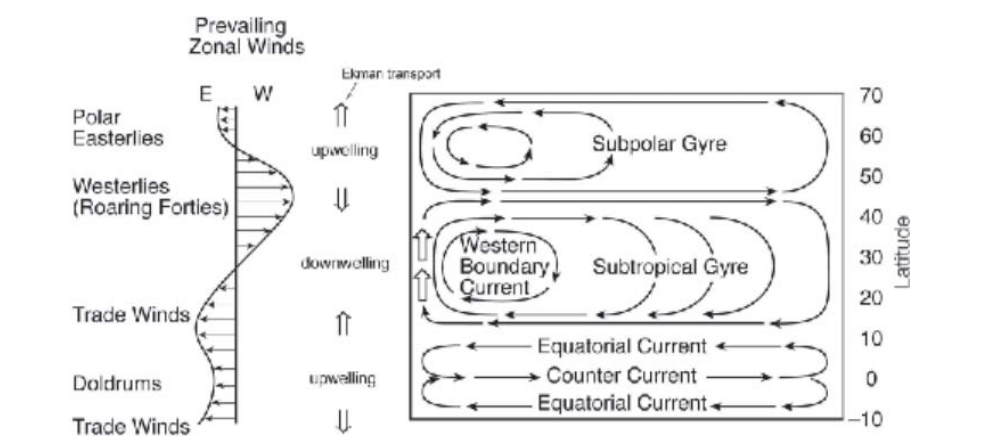
\includegraphics[width=\linewidth]{schematic_marshall_plumb.png}
 	\caption{Schematic of the barotropic stream function based on the Sverdrup relation. Showing the subpolar and subtropical Gyres and equatorial currents. Figure taken from \cite{MarschallPlumb}}
 	\label{fig:schem_currents}
 \end{figure}
\subsubsection{Passage throughflow}\label{sec:throughflowp}
For each of the passages mentioned in \prettyref{sec:bathys} it is interesting to talk about the total volume transport through each of the passages discussed in \prettyref{sec:bathys}. This is done using a simple integration to calculate the volumetric flux through each passage. This volumetric flux, defined as

\begin{align}
Q = \iint_A \vec{u} \cdot d\vec{A}
\end{align}	

For each passage a suitable location is chosen such that there are no boundaries next to the passageways, this is done for each time step. Then the $u$ component of the flow is used to compute the total flow. This method is the same for each of the passages and thus we can study the effect of changes in bathymetry to on the relative strength of the flow. However, it should be noted that these values may not represent real physical values. As the passages in a $4^{\circ}$ model are often only a few grid cells wide. Resulting in discrepancies in the calculation of the throughflow due to boundary conditions. 
There is however a more accurate way to calculate these throughflows. This can be done using the output of the Barotropic stream function discussed in \prettyref{sec:BSF_theory}. This also gives us a measure of (purely zonal) throughflow in each grid cell. It is however difficult to get accurate values from this in Veros because the current version does not display the boundary values for the stream function.

\todo[inline, color=green!40]{TODO: add a picture of each of the passages and the continent names + ocean names for reference}



Creating the bathymetries for the model was done using bathymetries from Muller et al.\cite{Muller2008Mar} these were scaled to a 4 degree model and subsequently changed to address passage openings in the 4 degree case where, due to the low resolution of the model, choices have to be made with respect to the opening of certain passages. One of the choices that was made specifically is to change the bathymetry of the standard 4 degree model to a custom one made in the same process as the other bathymetries too more accurately portray changes that occur using this process. One of the choices that was made is that the northern Sea is closed of in all of the bathymetries. This is mainly due to the fact that 4 degree models do not have enough resolution to support This sea and can cause strange behaviour to occur. Also there is little connection to the other oceans, thus negating the need for such a basin to be in our model.

The main events that shape the oceanic passages can be devided into time periods. These time periods are defined as follows in this paper. This deviates from their definitions in literature but serves only as a means of applying a name to the time steps.

\begin{table}[H]
	\begin{tabular}{lll}
		&From &Until \\
		Paleocene & 65Ma&55Ma    \\
		Eocene    & 50Ma&35Ma     \\
		Oligocene & 30Ma&20Ma    \\
		Miocene   & 20Ma&Present 
	\end{tabular}
\end{table}

%TODO (Relevant figures from paleoscene showing changes)
The model is started in the Paleocene where in the beginning a vast Pacific exists almost serving as a single basin. This period is largely characterized by the growth and development of a larger atlantic basin. Serving to decrease the size of the pacific basin. This can be seen in Figure %TODO add figures showing diffirence in size. 
Where the changes during the paleoscene are shown.
\begin{figure}[H]
	
	
	\centering
	\begin{subfigure}[b]{\linewidth}
		\centering
		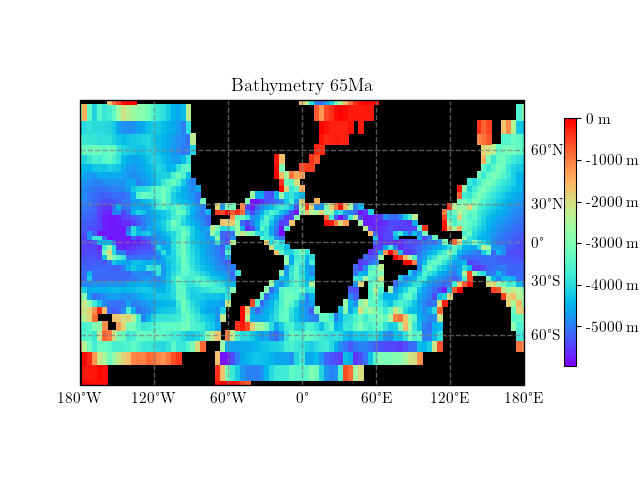
\includegraphics[width=\linewidth]{bathymetry/baath_65.png}
		\caption{Beginning of the Paleocene}
	\end{subfigure}
\begin{subfigure}[b]{\linewidth}
	\centering
	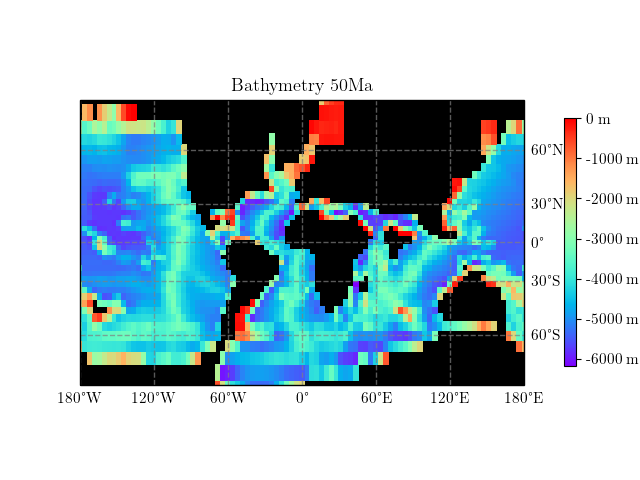
\includegraphics[width=\linewidth]{bathymetry/baath_50.png}
	\caption{End of the Paleocene}
\end{subfigure}
	\caption{}
	\label{fig:paleocene_bath}
\end{figure}


%TODO Eocene Drake-indian-tasman passages + depth

The Eocene in contrast to the Paleocene is destinguised by The opening of certain passages connecting oceanic basins. These effects are often studied extensively for each individual passage. Choosing the exact timespan for opening the passages is done manualy by looking at often active research takin into account big uncertaincies in the exact timing of the openings. The Eocene is characterized by several large events shown in Figure %todo add figure showing the events in detail
The first of such events that occurs is the indian continent colliding with the eurasian continent This has the effect of closing the deep water formations between the Thetys sea and the Indian ocean.
Next the Tasman passage is opened\cite{Lawver2003Sep} as a shallow passage slowly growing in size. The tasman passage opening is believed to have had a large impact on the onset of the ACC. The Total circulation of water around the antartic basin is finalized by the opening of the shallow Drake passage some 30Ma. 30Ma is specifically chosen to diffirentiate between the diffirent passage openings. Especially since there is still ongoing debate on the exact timing of drake passage opening.
%30ma drake passage opening (chosen as to diffirentiate between diffirent stages)
%35ma Indian passage closure
%35ma Tasman passage opening
%Indian continent colliding

%TODO Oligocene changes
The next time period is the oligocene Which is largely characterized by the deepening of the Tasman and drake passage and further expansion of the atlantic basin. It is believed %source
That the onset of the northern sinking atlantic started in this time period. Also the ACC probably is increasing in strenght.


%TODO Miocene

The miocene is Characterized by yet more increase in strenght of the ACC. Also Some more passage closures occur. Starting with the closure of the Thetys Seaway which had been decreasing in size in the previous 20Ma. Also the passage between modern day australia and indonesia is significantly decreasing in size due to the onset  of multiple vulcanic islands making the passage more narrow and shallow. Showing especially in this model. Further more the Thethys gateway
%0Ma current
%5Ma Wider Indonesia
%10ma last CAS
%14ma Thetys seaway last open 15ma first occurrence



Drake passage opening \cite{Scher2006Apr}

Tasman passage opening 

Central American seaway closure \cite{Molnar2008Jun} (deepwater 7Ma (10 for paper))\cite{Pindell1988Dec}

Tethys seaway closure \cite{Hamon2013Nov}

Widening of indonsian seaway (due to australia moving up.)


titis passage opening 

Choises made. 

Examples of where these choises interfere with reality.

Individual passages.

What age are we dealing with (Events/Changes observed in literature)


 



\newpage
\section{Results}

\subsection{Model runs}
The model ran for 500 years for each of the 14 timesteps. Accounting for a total of 7000 years of model time. The timings are shown in \cref{table:masteps}. We see that the total integration time is quite long but in general manageable. We note that it would have been possible to significantly speed up our work by using many nodes in parallel instead of a single node in succession. This would be required for higher resolutions but was not attempted here.
As a metric for the stability of the model, we look at the globally averaged salinity and temperature change over time. This tells us the drift of the model. In \cref{table:mastepstable} we see the drift over the last 10 years of integration. We see that all of the models seem to have a drift of less than $10\mathrm{e}{-4}^{\circ}C$ per year and a salinity drift less than $10\mathrm{e}{-4} psu$ per year.

\begin{table}[H]
	\centering
	\begin{tabular}{lllll}
Year & $\Delta time$ & $time$ & $\Delta T$& $\Delta S$\\
present day & 1'01" & 8:30& -2.1978& -1.8629\\
5Ma& 1'01" & 8:30& -2.8292& -2.5038 \\
10Ma & 1'01" & 8:30& -2.7764& -1.8219\\
15Ma & 1'02" & 8:40& -6.1497& -2.6299\\
20Ma & 1'01" & 8:30&  -5.3202& -1.9109\\
25Ma & 1'02" & 8:40& -5.3201& -1.9341\\
30Ma & 1'03" & 8:30& -3.0994& -1.5755\\
35Ma & 1'00" & 8:30& -0.3163&-1.6289\\
40Ma & 1'02" & 8:40& -5.1253& -1.7728\\
45Ma & 1'00" & 8:20& -5.1196& -1.7066\\
50Ma & 1'00" & 8:20& -4.9925& -1.6592\\
55Ma & 1'01" & 8:30& -4.9158& -1.6586\\
60Ma & 1'02" & 8:40& -5.5853& -1.6902\\
65Ma & 1'03" & 8:50& -6.3302& -1.8980\\
	\end{tabular}

\caption{$\Delta time$ is the time per integration in minutes'seconds". $time$ is the time in hours:seconds for each run. $\Delta T$ is the average temperature gradient for the last 10 time steps in $10^{-4} C$ per year. $\Delta S$ is the average salinity gradient for the last 10 time steps in $10^{-4} psu$ per year.}
\label{table:mastepstable}
\end{table}


\subsection{Control setup}


To get an understanding of the quality of the model and thus if any of the results resemble reality, one can compare the present-day setup of the model to an existing model with realistic forcings. Also, the model can be compared to another similar higher resolution model. This can be a useful tool to see what aspects of the present-day situation are captured by the model and more importantly which nuances are lost. General circulation models with a resolution comparable to the model used in this paper often loose major features having to do with the overturning circulation (\cite{stone1990limitations}). Especially the restoring boundary conditions at the surface are troublesome where capturing artifacts of the thermohaline circulation is highly dependent on surface salinity and temperature profiles. This dependence is even further complicated by the highly idealized forcings used here (\cref{sec:forc_err}). To get a qualitative look at the error introduced in our model, the BSF and the MOC outputs are studied together with their temperature profiles. We compare our control setup with a run of our model with the original \cite{ECMWFForc} forcings scaled to 4-degrees. These are the same forcings used as a basis for making the idealized forcings as mentioned in \cref{sec:forcing_ideal}.
\begin{figure}[H]
	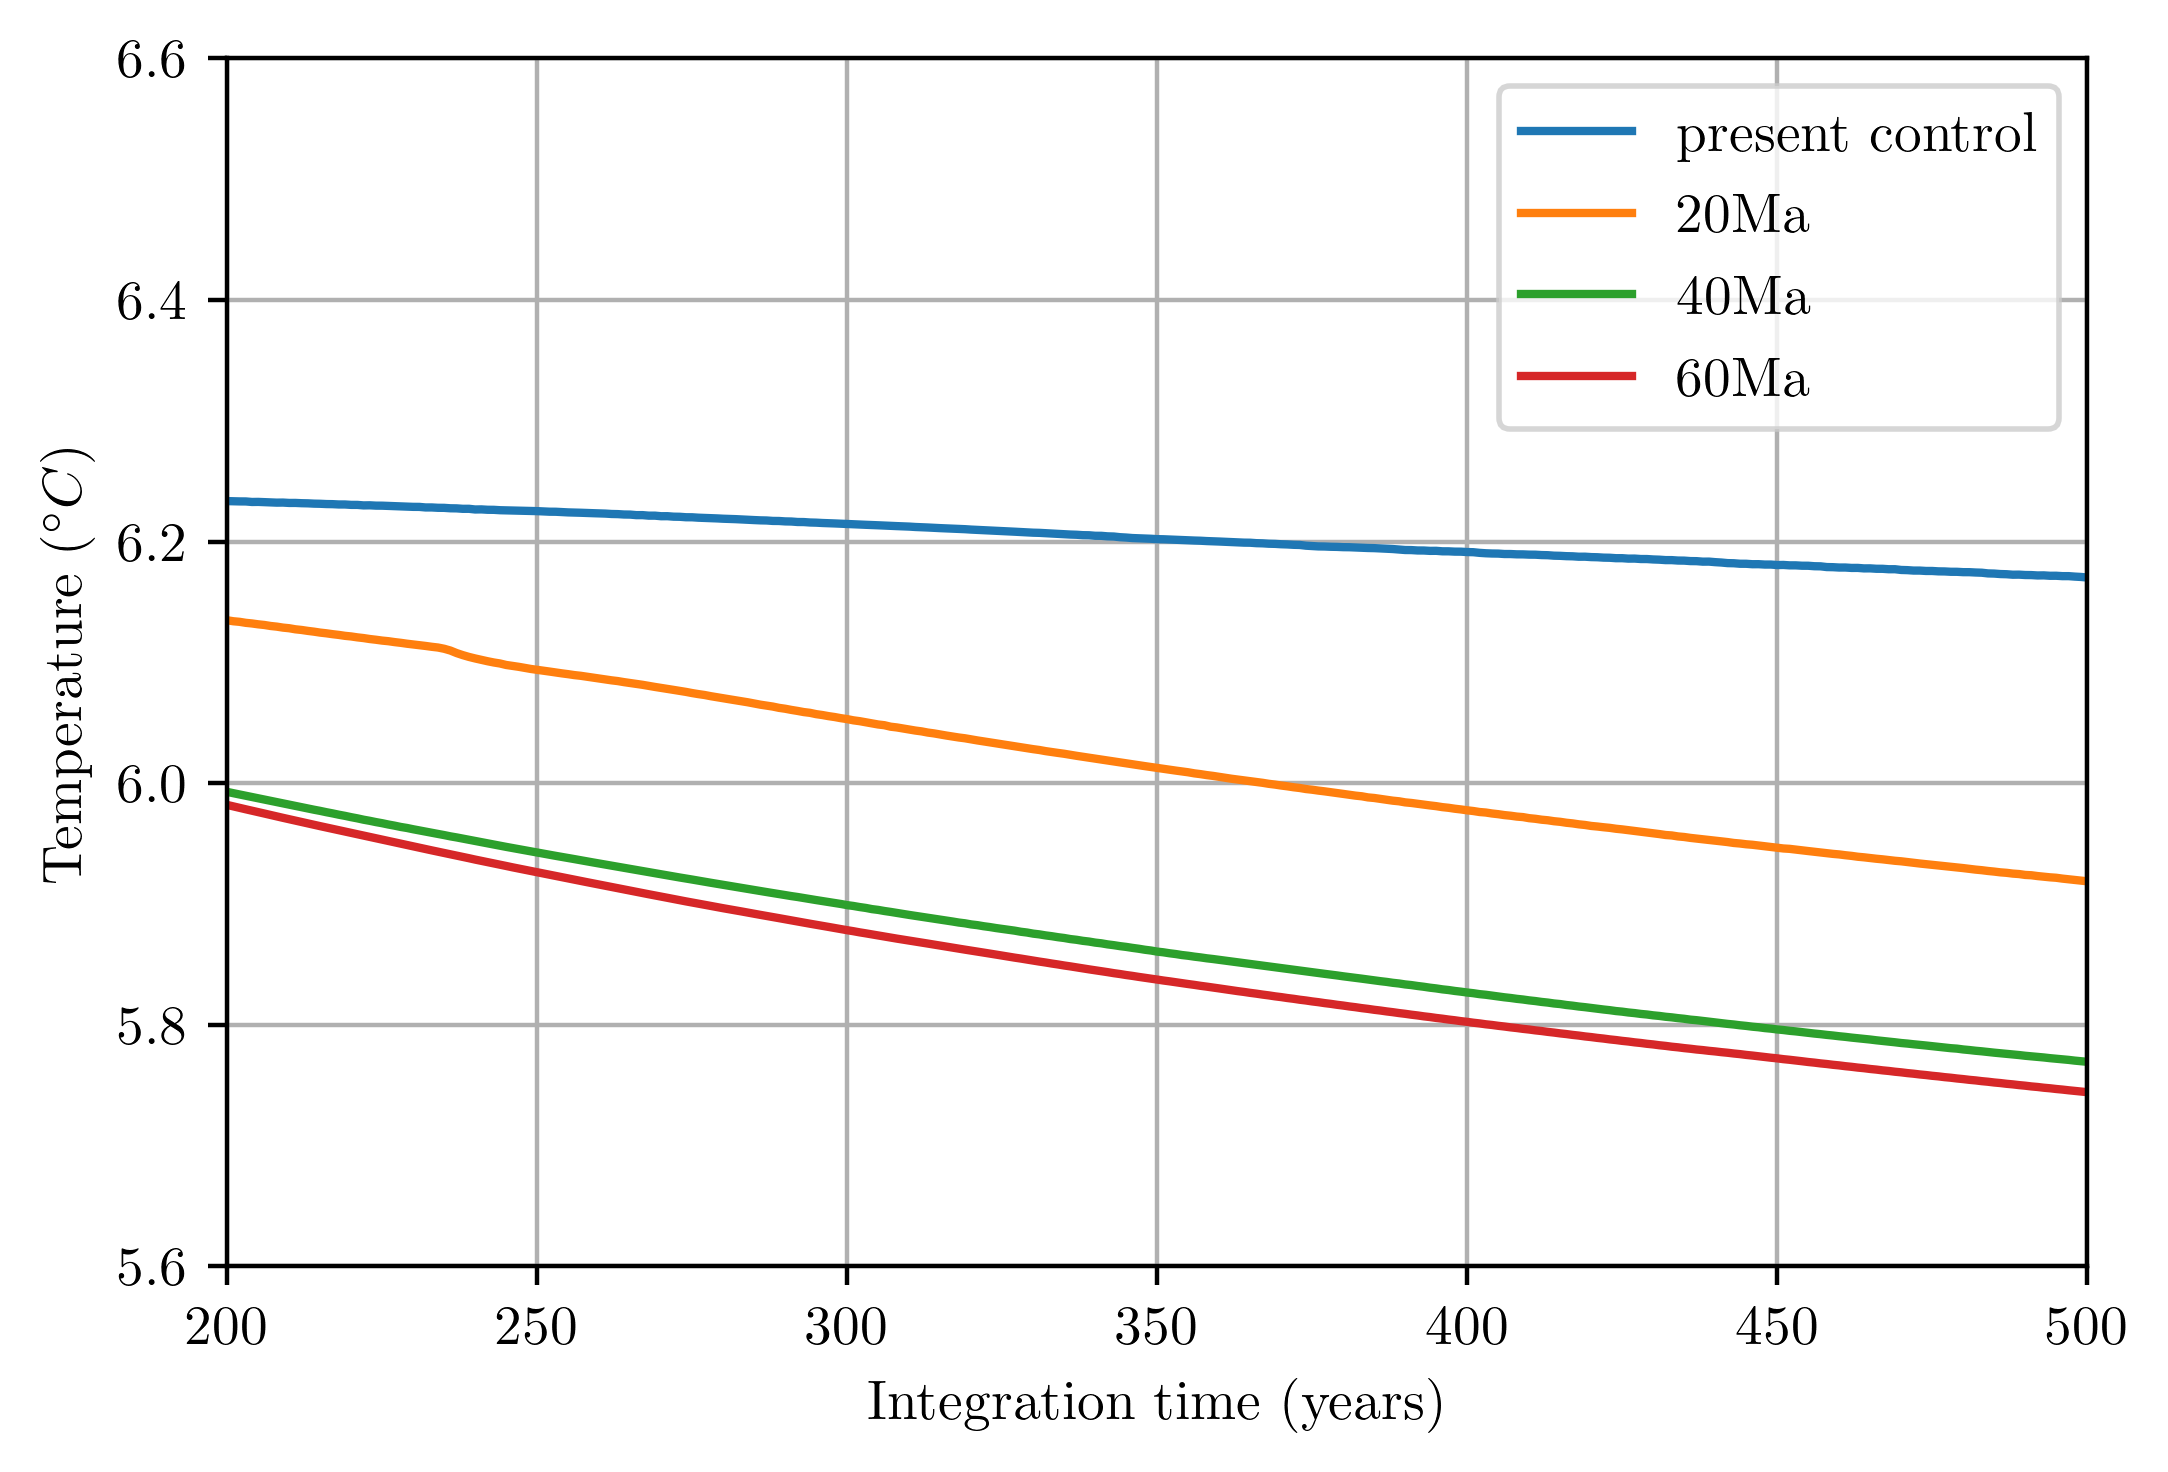
\includegraphics[width=\linewidth]{drift_integration.png}
	\caption{Total globally averaged temperature ($^{\circ}C$) for Present day (blue), 20Ma (orange), 40Ma (green) and 60Ma (red). From 200 to 500 years integration.}
	\label{fig:avtempgrph}
\end{figure}
\subsubsection{BSF control}
Too look at the quality of the barotropic stream function we compare the barotropic stream function with the control. In \cref{fig:bsf2_compared} we see the barotropic stream function compared. Here we see quite a few differences. Notably, the strength of the gyres is much weaker in our simplified forcings case. This can mostly be explained by the generally weaker wind stresses in these regions. Also, in our simplified model there is a notable absence of the sub polar gyre in the northern Atlantic. The difference in strength of the subtropical gyres is about $10Sv$ on average. Reaching a $20 Sv$ difference in the subtropical gyre in the Indian ocean. 


% Only showing a weaker subtropical gyre in the Indian ocean and a weaker gulf stream. In the temperature profile at 245 meters in depth there are however larger discrepancies. There is a $4^{\circ}C$ difference in temperature in the gulf stream and a $2^{\circ}C$ temperature difference in the Kuroshio gyre. This can be attributed to weaker SST forcing at the surface on these places because of the zonal mean nature of these forcings and also due to the shorter runlength of the model. Thus the model did not yet get addequate time to fully develop the flows (THIS COULD BE BETTER)


\end{multicols}
%example full width overturnings

\begin{figure}[H]

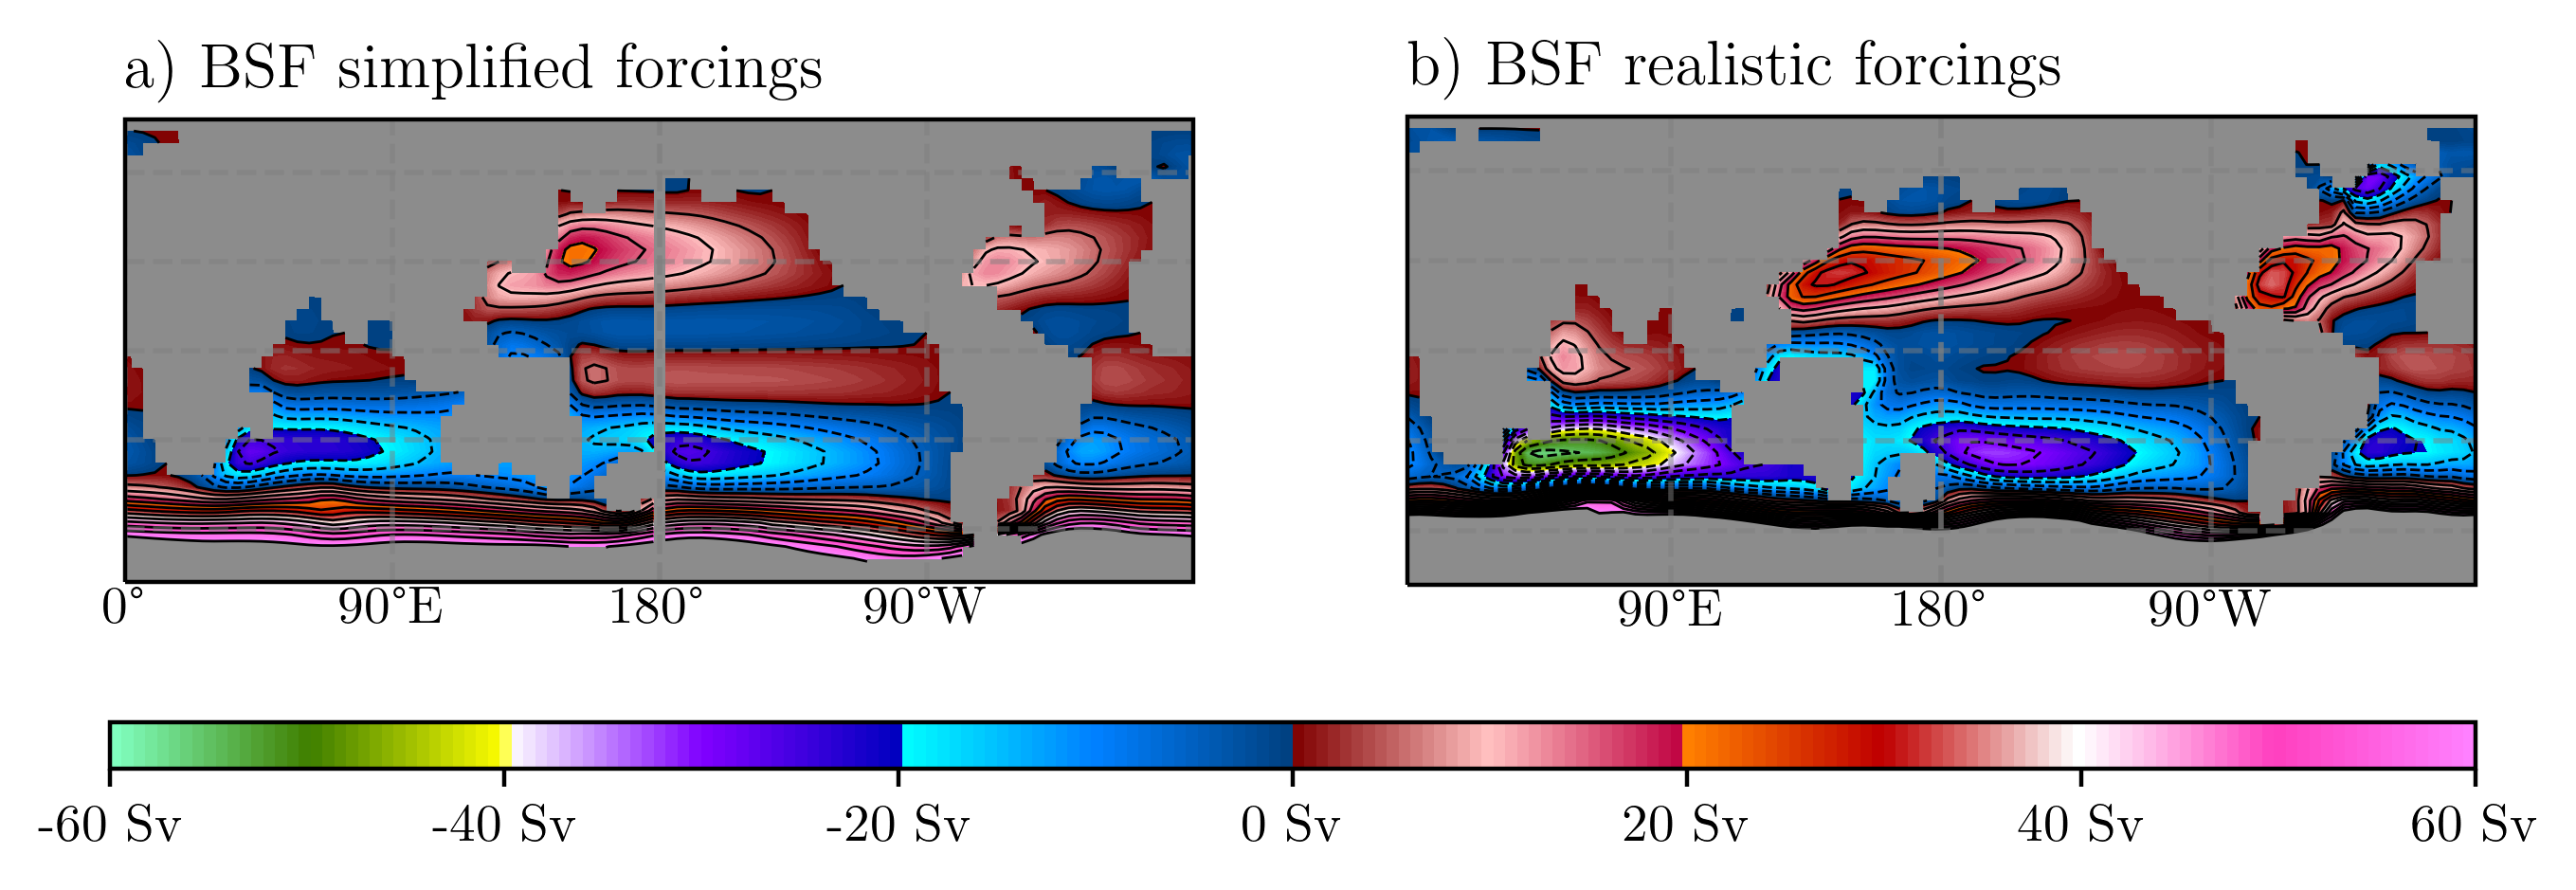
\includegraphics[width=\linewidth]{bsf_real_non.png}
\caption{Barotropic stream function with contours every 5 Sv. For \textbf{a)} simplified forcings and \textbf{b)} realistic forcings.}
\label{fig:bsf2_compared}
\end{figure}
\begin{figure}[H]
\begin{subfigure}{0pt}
	\caption*{}
	\label{fig:mocCompA}
\end{subfigure}
\begin{subfigure}{0pt}
	\caption*{}
	\label{fig:mocCompB}
\end{subfigure}
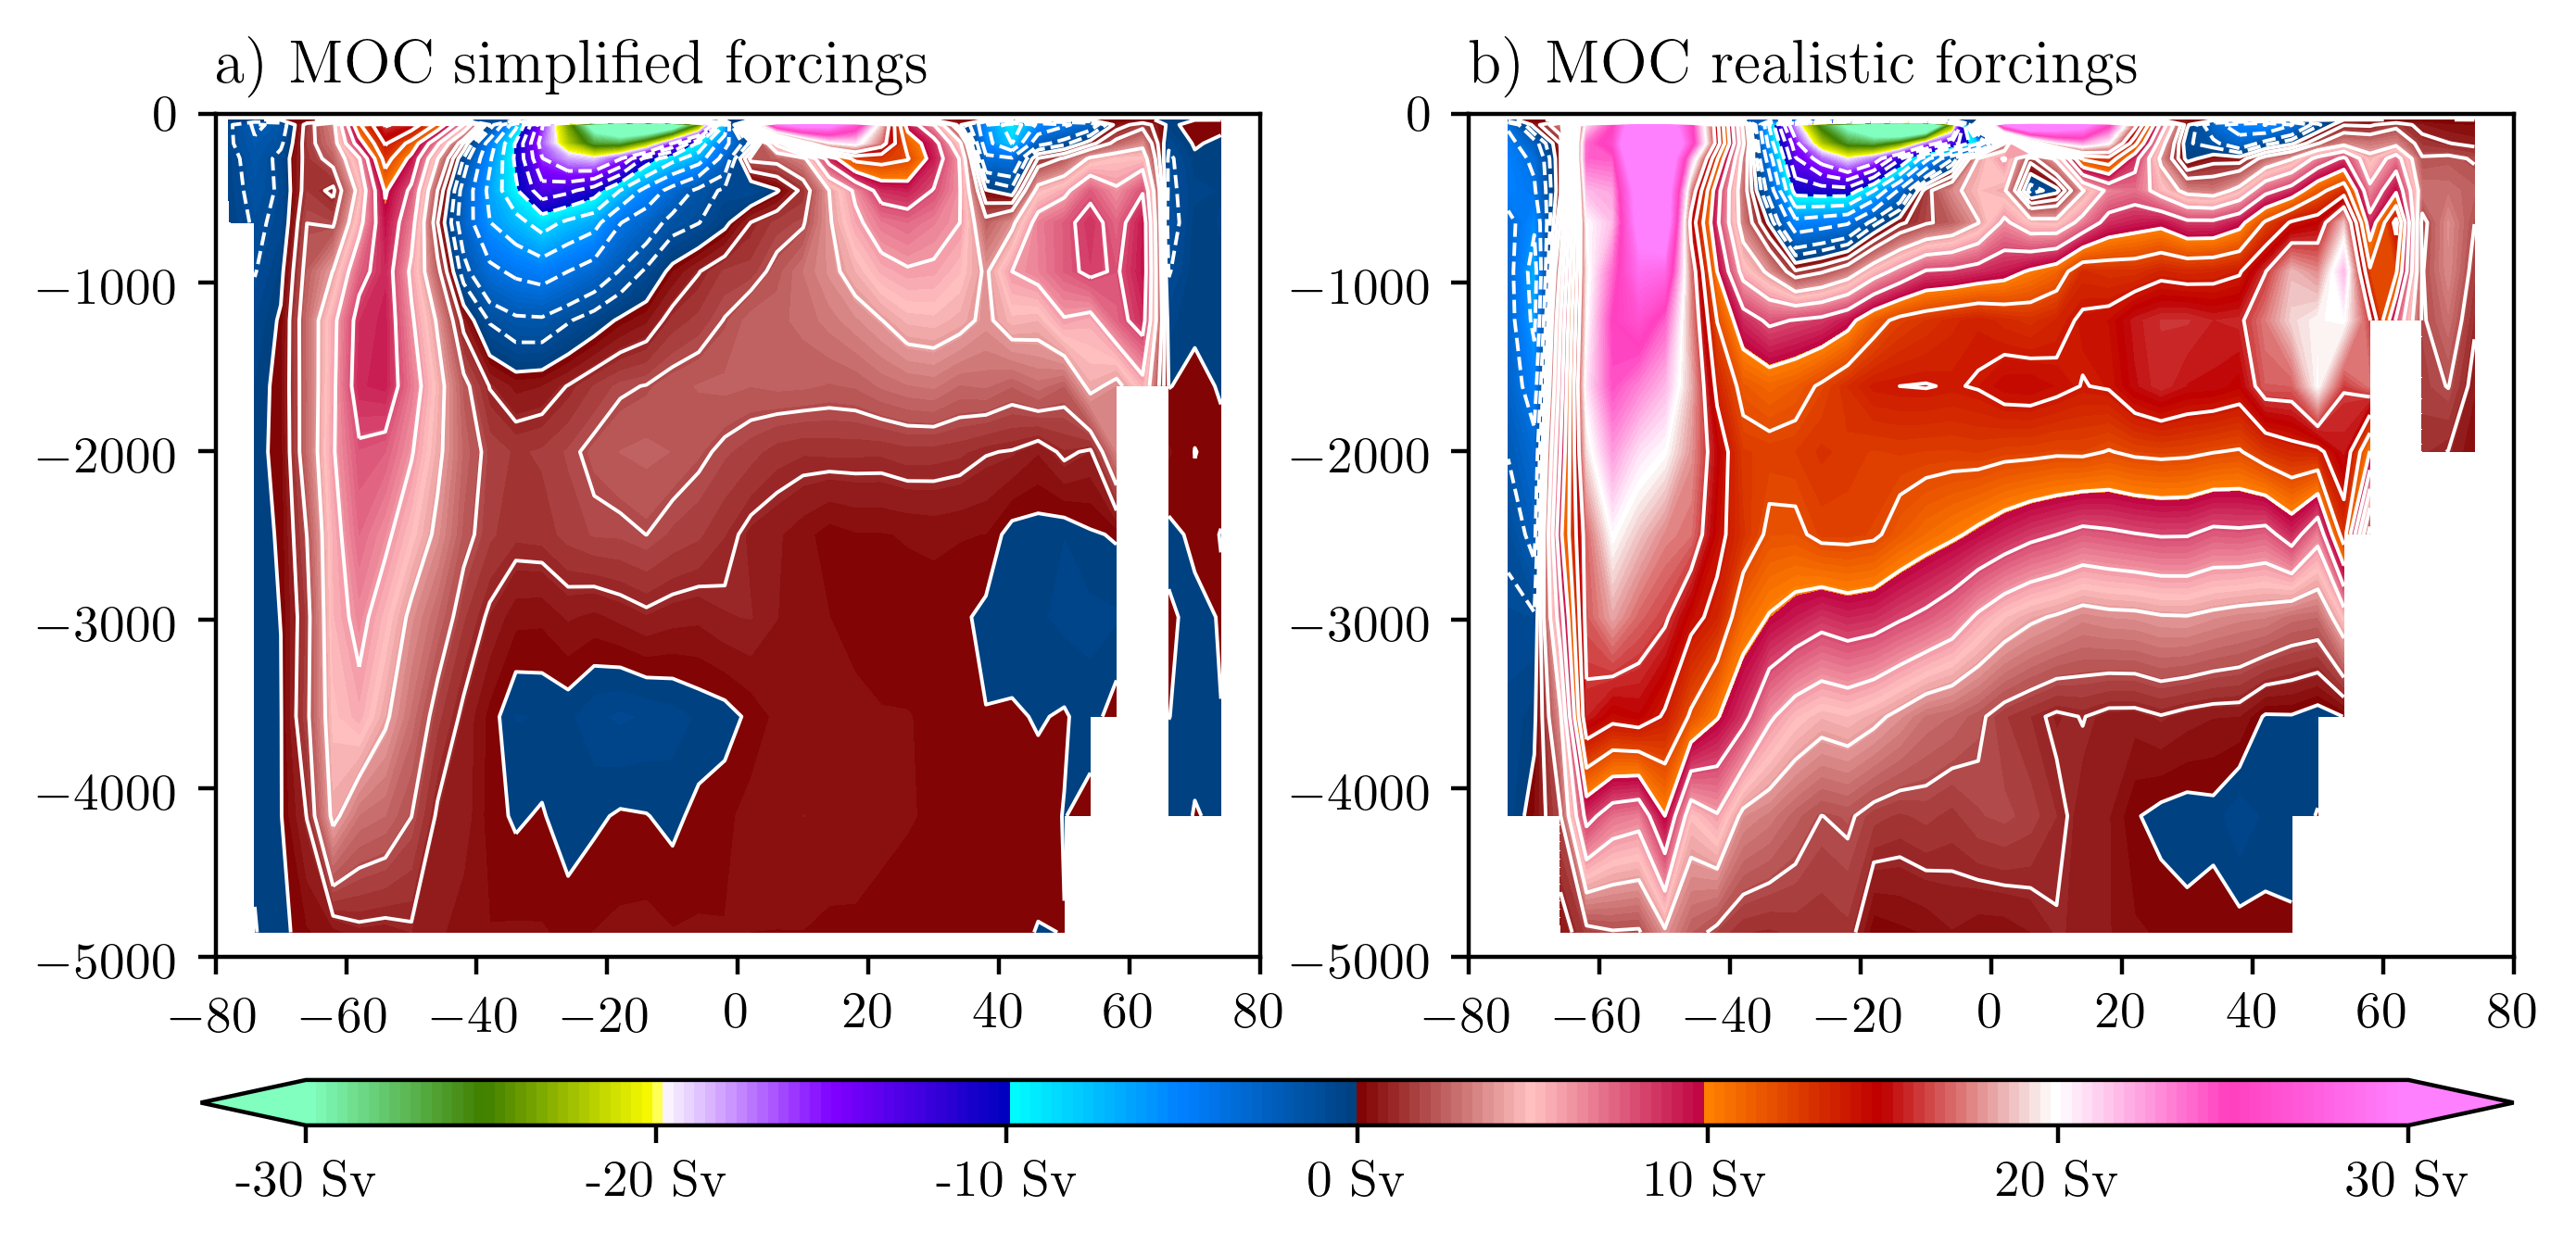
\includegraphics[width=\linewidth]{moc_forcings_real_fake.png}

\caption{MOC stream function with contours every 2 Sv. For \textbf{a)} simplified forcings and \textbf{b)} realistic forcings. Negative values (dashed lines) indicate counterclockwise circulation}
\label{fig:moc_compared}
\end{figure}

\begin{multicols}{2}

\subsubsection{Quality of the MOC} \label{sec:mocQual}
Next, we look at the MOC stream functions and compare them between the two models. Here we must note the difference in geometry between the two models. This is because we use an interpolated version in the simplified forcings case. That is different from the geometry used by Veros. In \cref{fig:moc_compared} we see the MOC stream function for the simplified and realistic models. Here the real problem of using simplified forcings is visible. The overturning circulation with the simplified forcings is extremely weak compared to the overturning circulation with simplified forcings. Compared to the model with realistic forcings in \cref{fig:mocCompB} we see that the NADW cell is much weaker in \cref{fig:mocCompA}. 

We note that several key features are not captured by both models. The first, most striking feature is the complete absence of the AABW cell. This is a common feature of low-resolution models used here. Furthermore it is noted that the absence of accurately simulated sea ice in both models contributes further to the quality of the southern ocean simulations. We also see a very large cell in the southern ocean around $60^{\circ} S$. This is a purely wind-driven cell not seen in the more realistic overturning from \cref{fig:moc_ex}. It is known as the "Deacon cell" (\cite{sverdrup1942oceans}; \cite{deacon1933general}).

For each of the afforementioned passages the throughflow was computed. This is done using a simple integration to calculate the volumetric flux through each passage.
\begin{align}
	Q = \int \int_A \vec{u} \cdot d\vec{A}
\end{align}	
For each passage a suitible location was chosen such that there are no boundaries next to the passageways. Then the $u$ component of the flow is used to compute the total flow. This method is the same for each of the passages and thus we can study the effect of changes in bathymetry to on the relative strenght of the flow. However, it should be noted that these values may not represent real physical values. As the passages are often only a few gridcells wide and, the nature of the 4 degree model. Resulting in discepencies due to boundary conditions. The passageways have been labeled in figure (figure of these) and results are plotted in figure (figure of these).

\begin{figure}[H]
	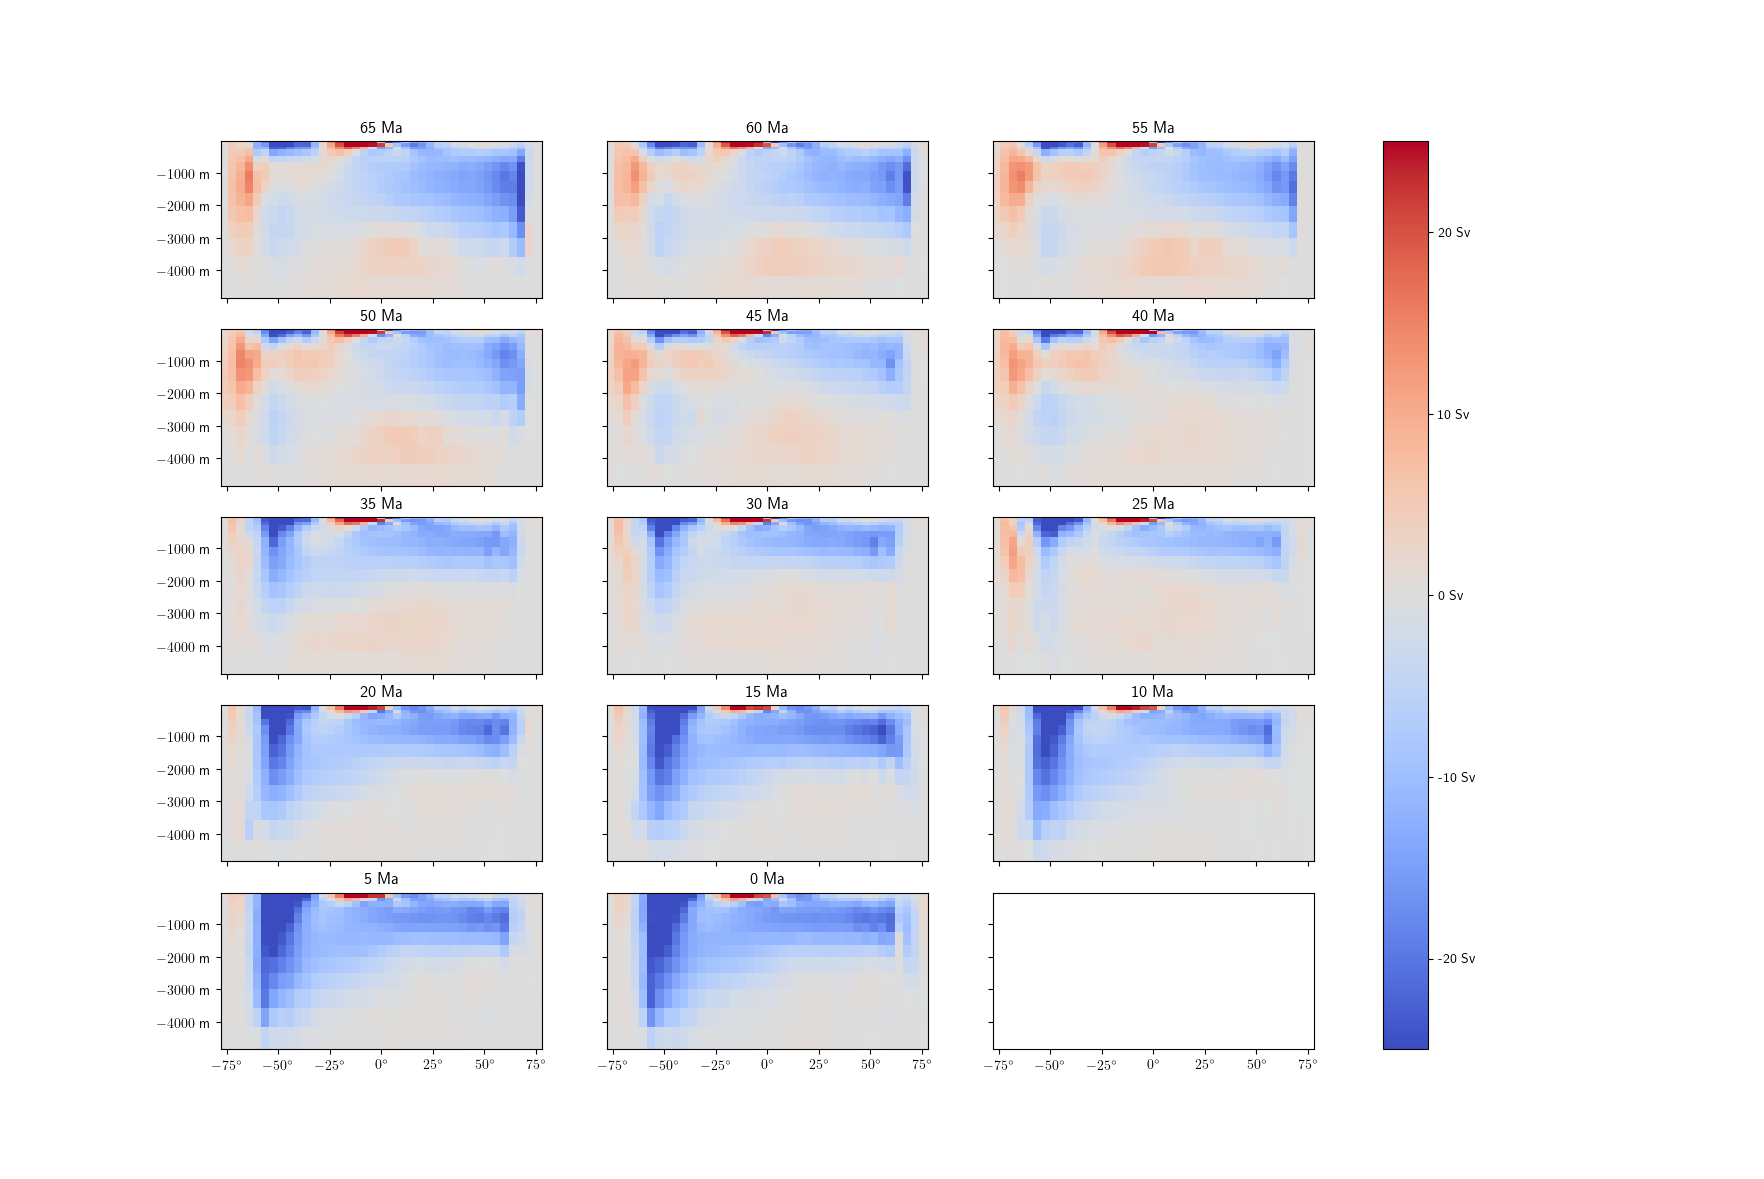
\includegraphics[width=\linewidth]{overturning_overview.png}
	\caption{test caption}
	\label{fig:example1}
\end{figure}

\end{multicols}
%example full width overturnings

\begin{figure}[H]
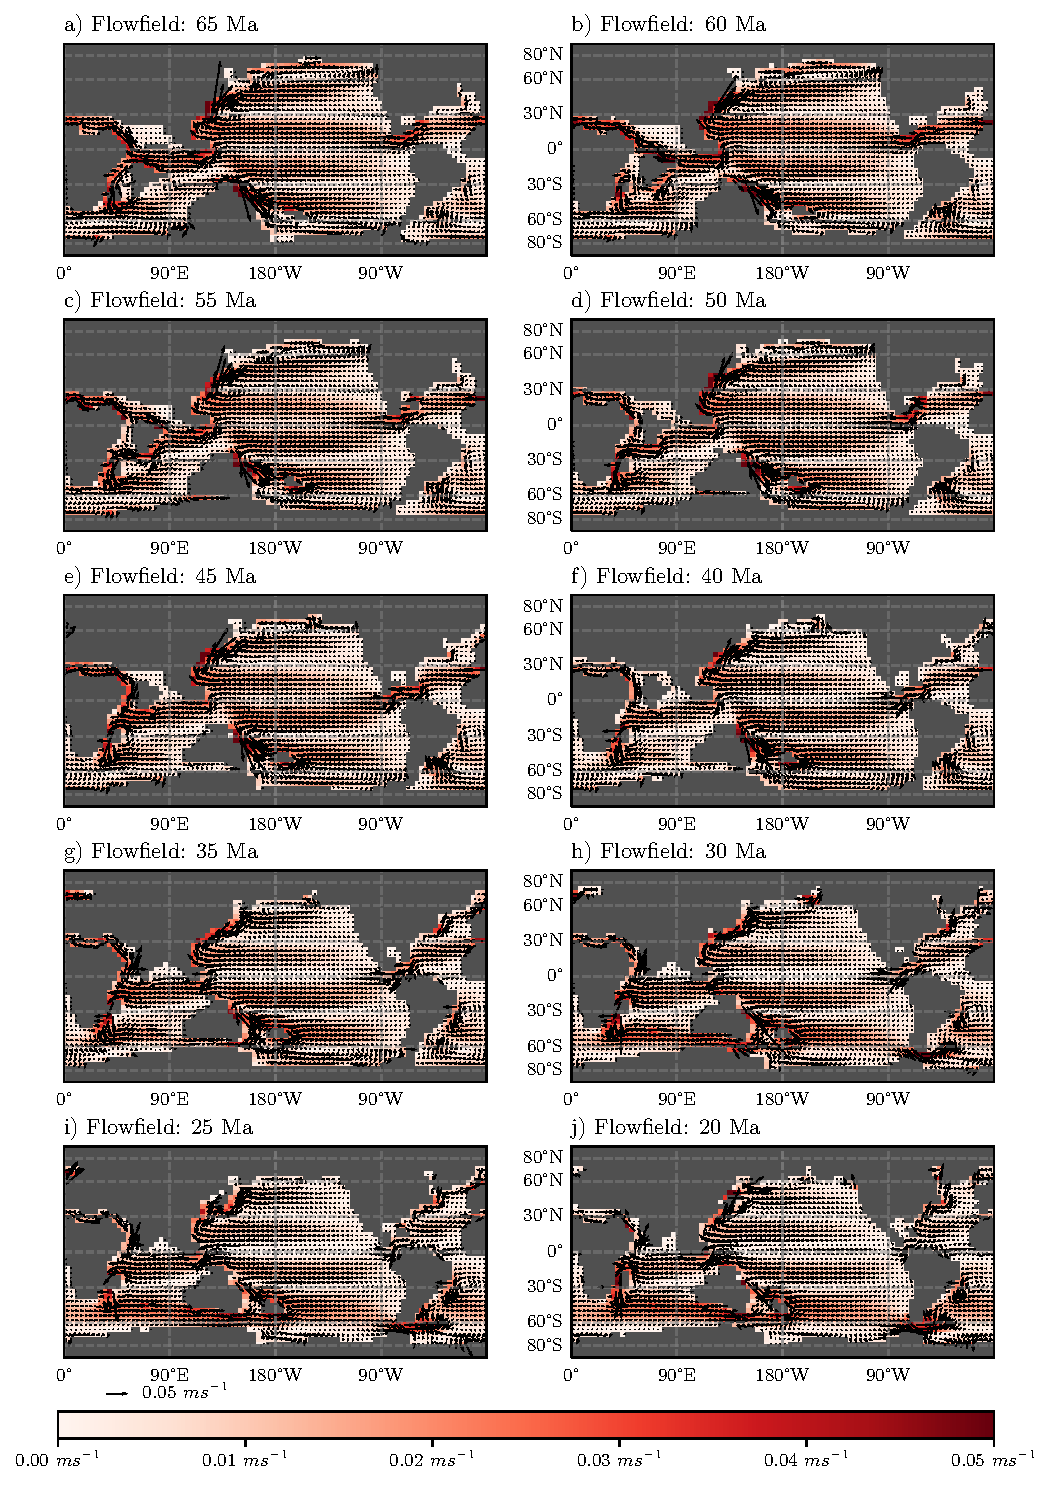
\includegraphics[width=\linewidth]{flowfield_1.pdf}
\end{figure}
\begin{figure}[H]
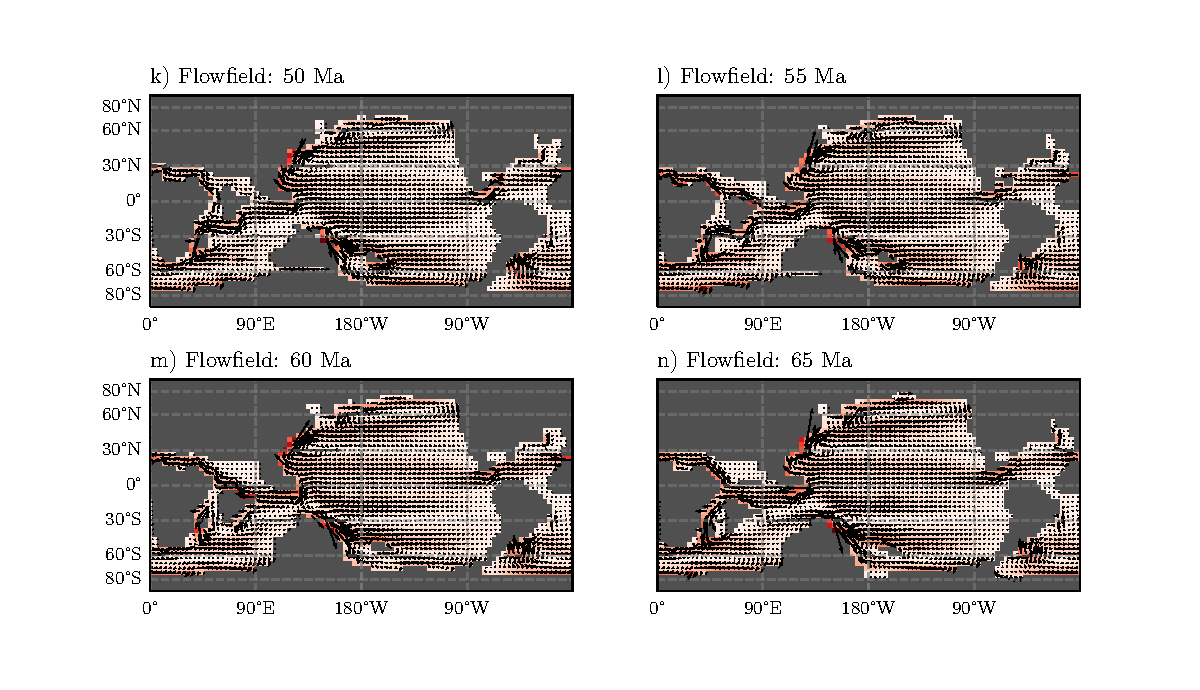
\includegraphics[width=\linewidth]{flowfield_2.pdf}
\caption{Flow field for each time step, showing the velocity of the vertical column as vectors. The values are in $m s^{-1}$}
\label{fig:flowfield}
\end{figure}

\begin{multicols}{2}
\subsection{Barotropic Stream function}
\label{sec:BSF}

Next we will look at the barotropic stream function for each of the time steps discussed here. Some of the flows that are discussed in this section are closely related to the flows explained in \fref{sec:throughflow}. Here we will have a stronger focus on the flows gyres seen in the ocean and their relative strength in a time sense. Each of the oceanic basins is discussed in detail. An overview of each of the barotropic stream functions can be seen in \fref{fig:bsf_total}. It is very visible that the boundary conditions of the BSF are not shown here. This is due to the previously stated fact that they are excluded from the model output produced by Veros. It must however be noted that this does not mean that flows through the passages are not modeled but rather only that the passages themselves do not show up on the plots of the barotropic stream function. In this case the barotropic stream function serves only to see the major ocean gyres and how water is transported in these gyres.

\subsubsection{Indian Ocean}

\subsubsection{Pacific Ocean}
The pacific ocean is of particular interest in this case. It is easily vi
\subsubsection{Atlantic Ocean}



%The detachment of Australia to the antarctic current at 35Ma introduces a strong flow ($17Sv$) through the newly formed Tasman passage. However there is no

\end{multicols}
%example full width overturning
\begin{figure}[H]

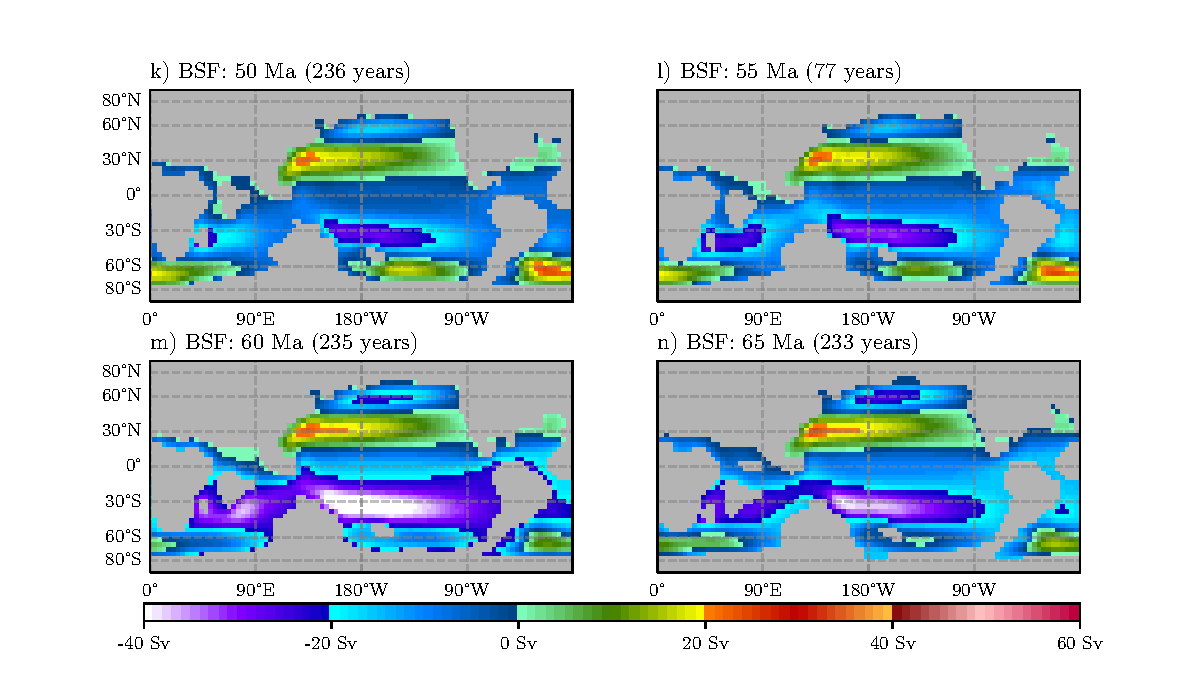
\includegraphics[width=1\linewidth]{BSF_1.pdf}
\end{figure}
\begin{figure}[H]
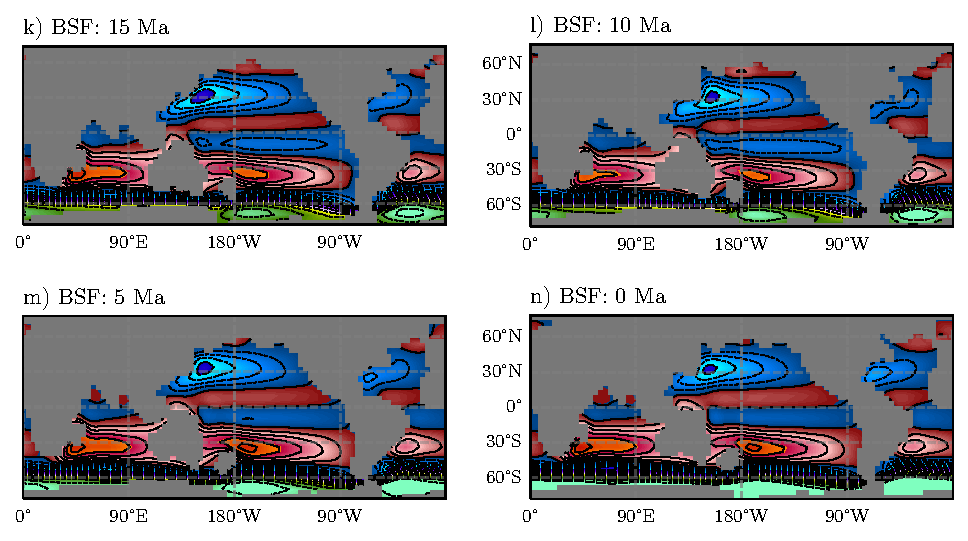
\includegraphics[width=1\linewidth]{BSF_2.pdf}
\caption{Barotropic Stream Function with contour lines every $5 Sv$}
\label{fig:bsf_total}
\end{figure}

\begin{multicols}{2}

Next we will do an analysis on the Global Meridional overturning current stream function (MOC). As mentioned in \prettyref{sec:MOCSTREAM} these values will probably not result in a very realistic picture of the overturning circulation. However it still gives us a rough general idea of the deep ocean flows of the thermohaline circulation. This section will again be split into the time periods as defined in \prettyref{sec:bathys}.

\subsubsection{Paleocene}
%65-55
In the Paleocene one of the most interesting aspect is the southern cell extending from the equator to the antarctic continent. A strong ($9 Sv$) southern cell exists. This cell is largely responsible for the mostly positive nature of the overturning circulation seen in the BSF.

(need to research more)


\subsubsection{Eocene}
%50-35
In the eocene we observe little diffirence to the streamfunction in the paleocene. The most interesting feature is the onset of the previously mentioned "proto ACC" in which the southern cell extends downwards. This indicates that the proto ACC might be captured by the model.


\subsubsection{Oligocene}
%30-20
The oligocene is characterized by the strong onset of the ACC and a subsequent decrease in size of the south polar cell. It being "pushed" aside due to the strong ACC currents. Another interesting artifact of this is that in the $30 Ma$ setup a kind of overturning current is observed. This is however not shown in the 25 and 20 Ma time steps. It should be noted that the deep water cells (<-2000 m) in all of these are still too weak to be of any realistic value. The Oligocene does seem to harbour some of the strongest Polar cells in any of the models. This was not necicarily observed in the Pictures of the BSF.

\subsubsection{Miocene}
%20-0

The miocene shows some of the main features of the MOC. One of these is the overturning current previously mentioned. It is however important to note that it is still really weak compared to other models with more depth layers and observations (\cite{von2006effect}). Probably due to the fact that the overturning circulation in the Atlantic is absent in this model. This may simply be a case of boundary conditions but could also be explained by the relatively weak SSS forcings in the Atlantic compared to real world values. In the last 15 Ma we see very little change overall in the MOC stream function. We see mostly fluctuations in the northern sub polar cell. 

\end{multicols}
%example full width overturning
\begin{figure}[H]

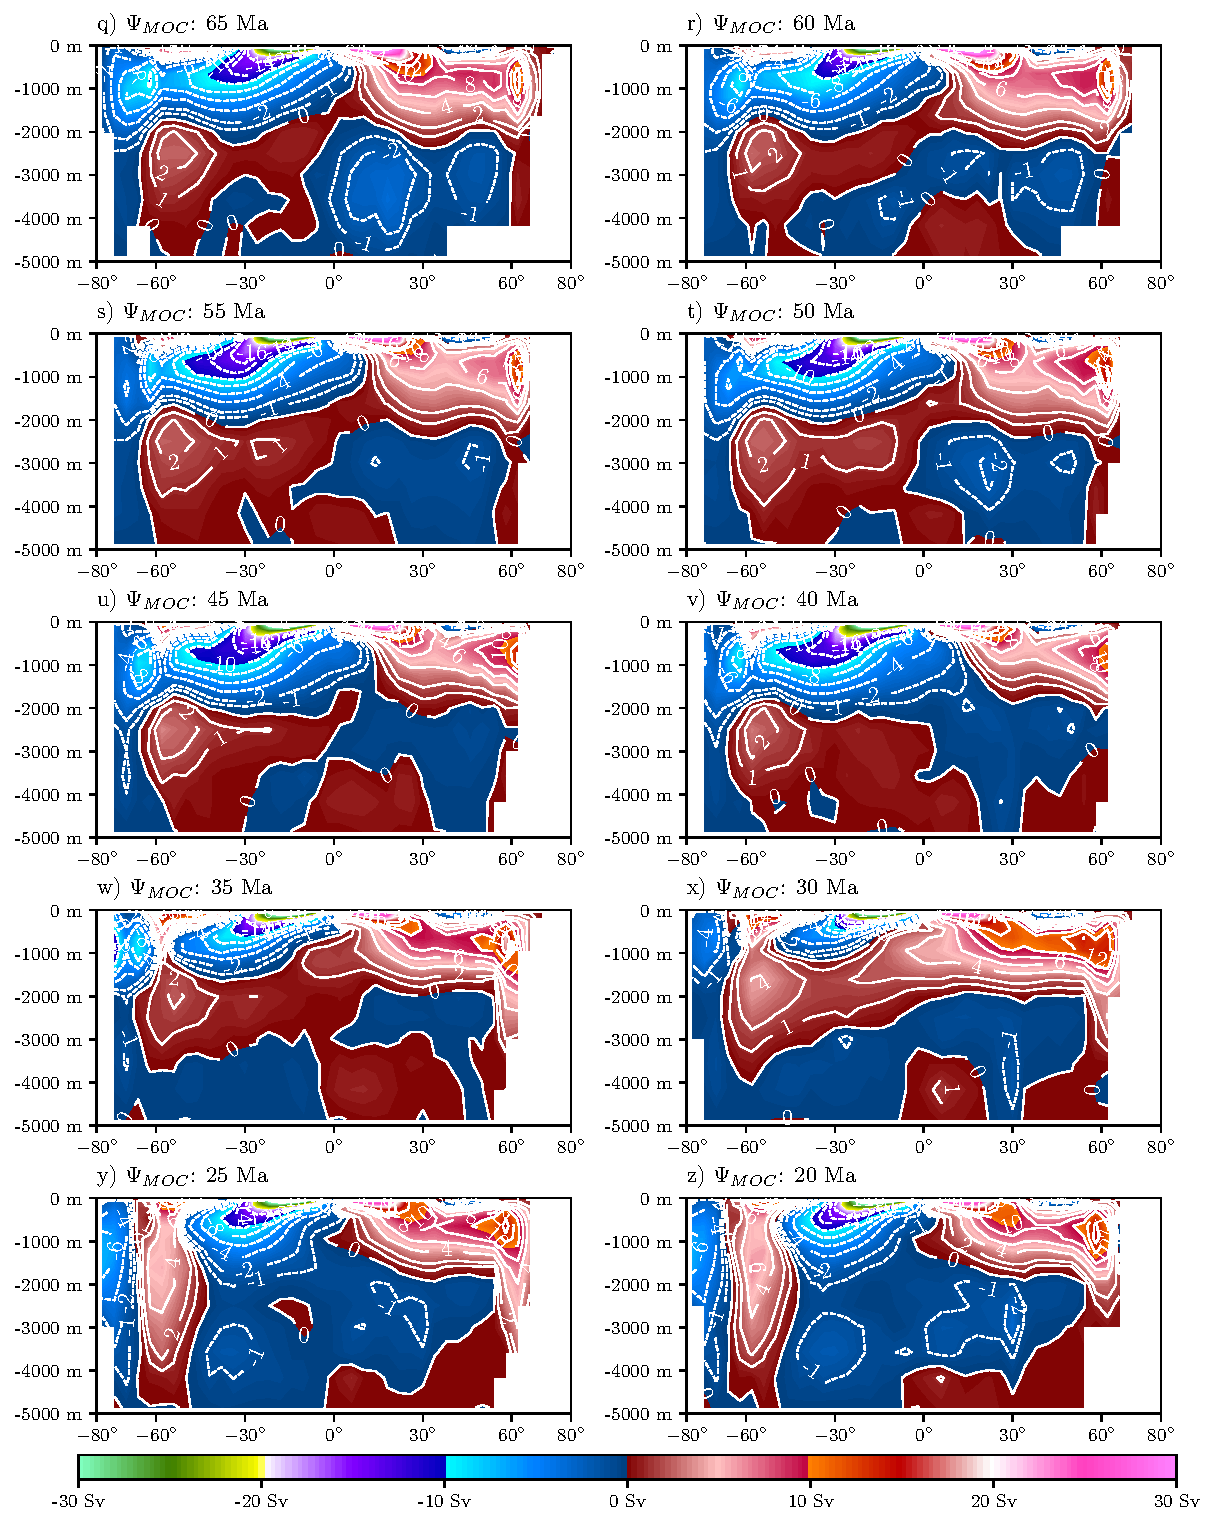
\includegraphics[width=1\linewidth]{MOC_1.pdf}
\end{figure}
\begin{figure}[H]
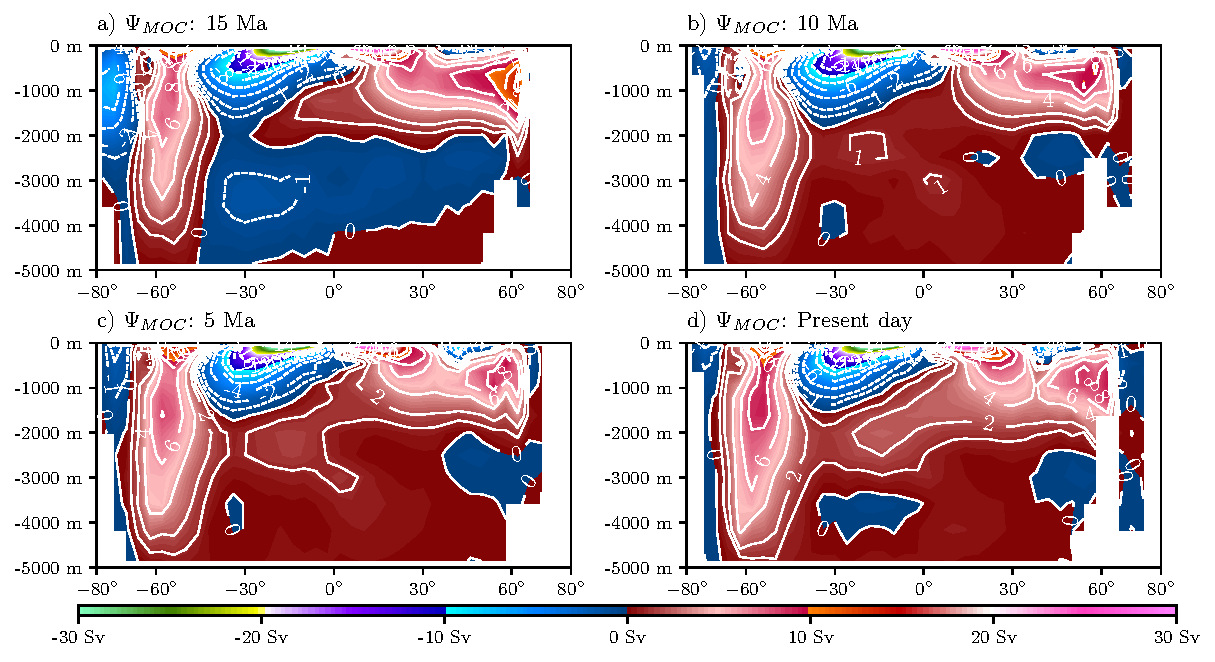
\includegraphics[width=1\linewidth]{MOC_2.pdf}
\caption{Barotropic Stream Function}
\label{fig:moc_total}
\end{figure}

\begin{multicols}{2}


\subsection{Temperature and Salinity Changes}\label{sec:temp+sal}
To get a better picture of the changes that occur during the time periods we compare differences in sea temperature and salinity at 250m depth between the models. We do not use the sea surface temperature and salinity here because of the restoring boundary conditions used on the top layer of the ocean. It is important to note that these restoring boundary conditions with the simplified forcings make a discussion on the thermohaline circulation to be of limited value. But we can get an idea of what general changes occur. For a full overview of the salinity and temperature profiles the reader is referred to the appendices at the end of this paper.

First, we compare the differences between the 55Ma basin and the 35Ma basin (\cref{fig:5535cooling}). Here we see substantial differences between the two. One of the key features of the Eocene seems to be a large amount of cooling in the southern Atlantic along with a heating of the southern pacific. We also see that the Salinity changes closely match the locations of the Temperature increases. However, this is less noticeable in the northern Atlantic where the change in salinity is relatively smaller.


\begin{figure}[H]
	\begin{subfigure}[b]{\linewidth}
		\caption{}
		\label{fig:5535cooling}
		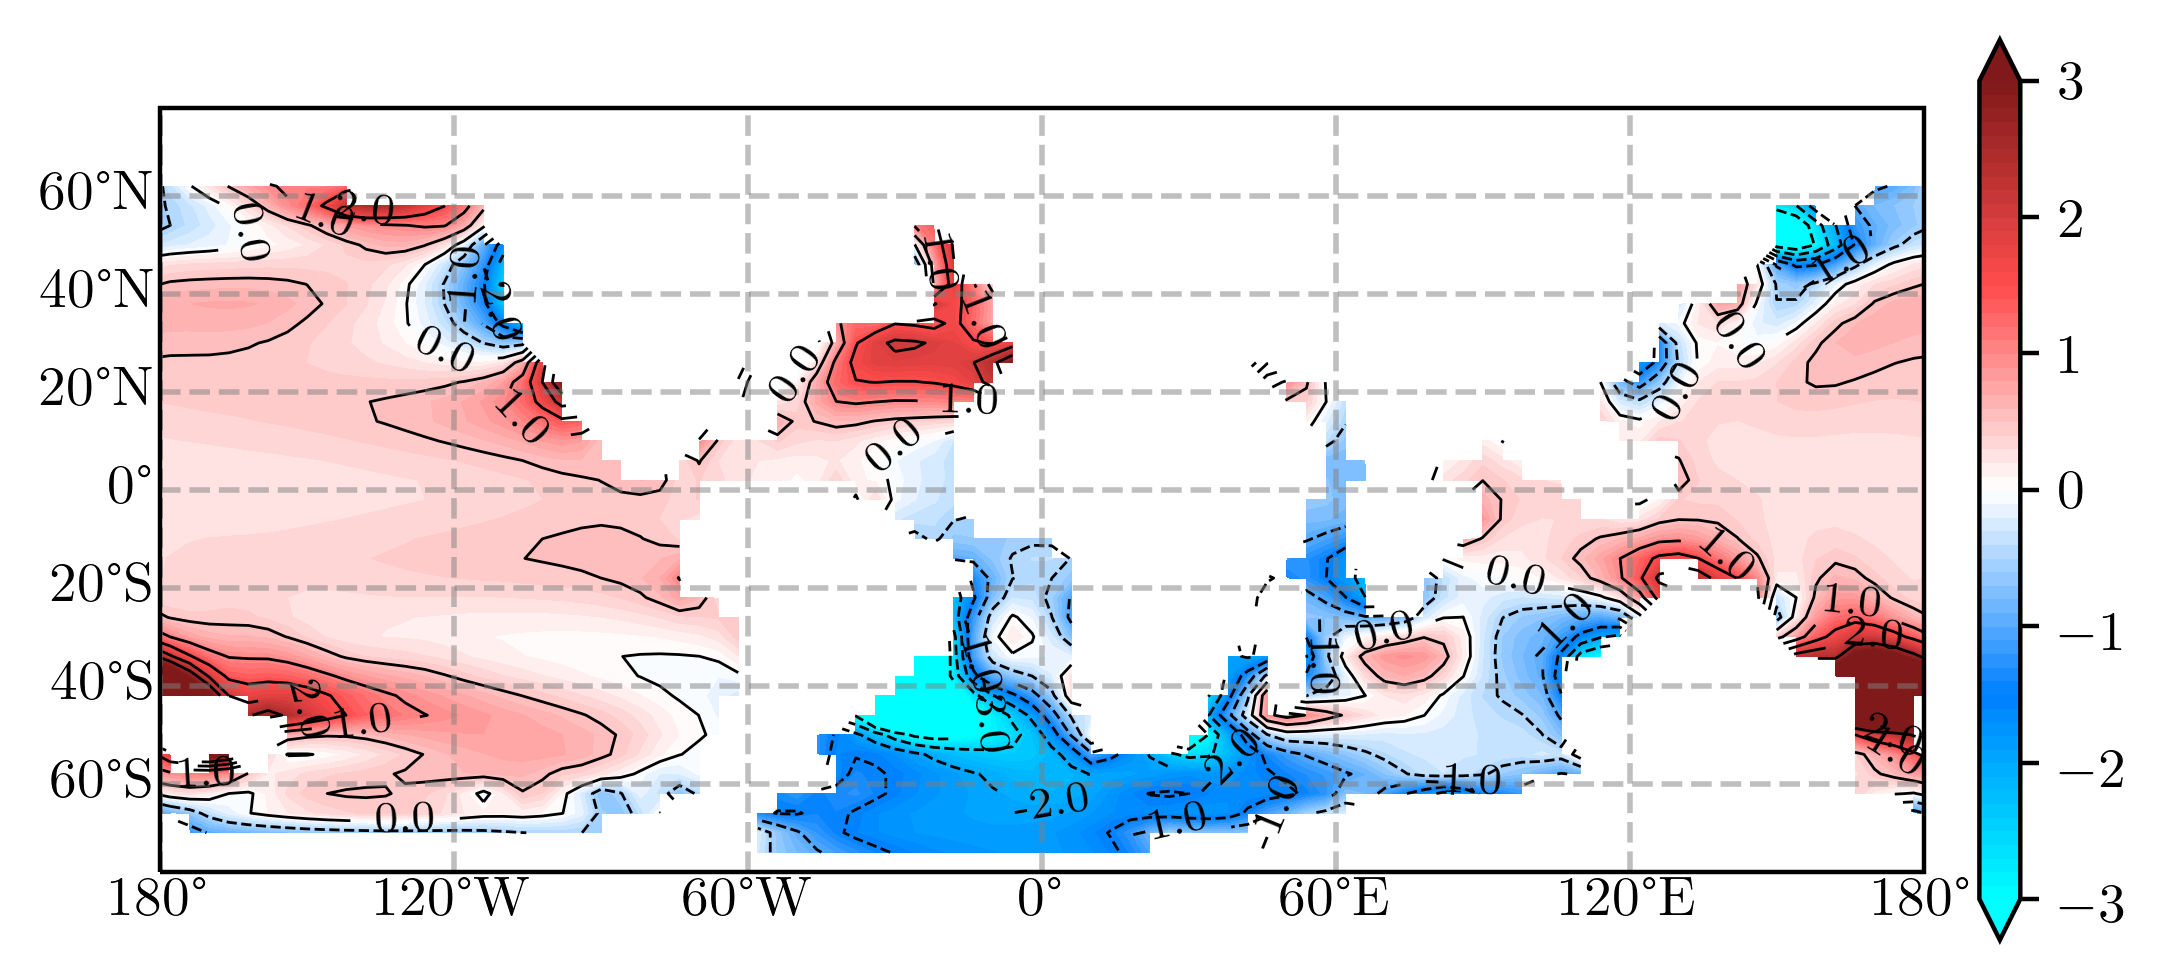
\includegraphics[width=\linewidth]{Paleo_eocene_55_35.png}
		
		
	\end{subfigure}
	\begin{subfigure}[b]{\linewidth}
		\caption{}
		\label{fig:salt5535cooling}
		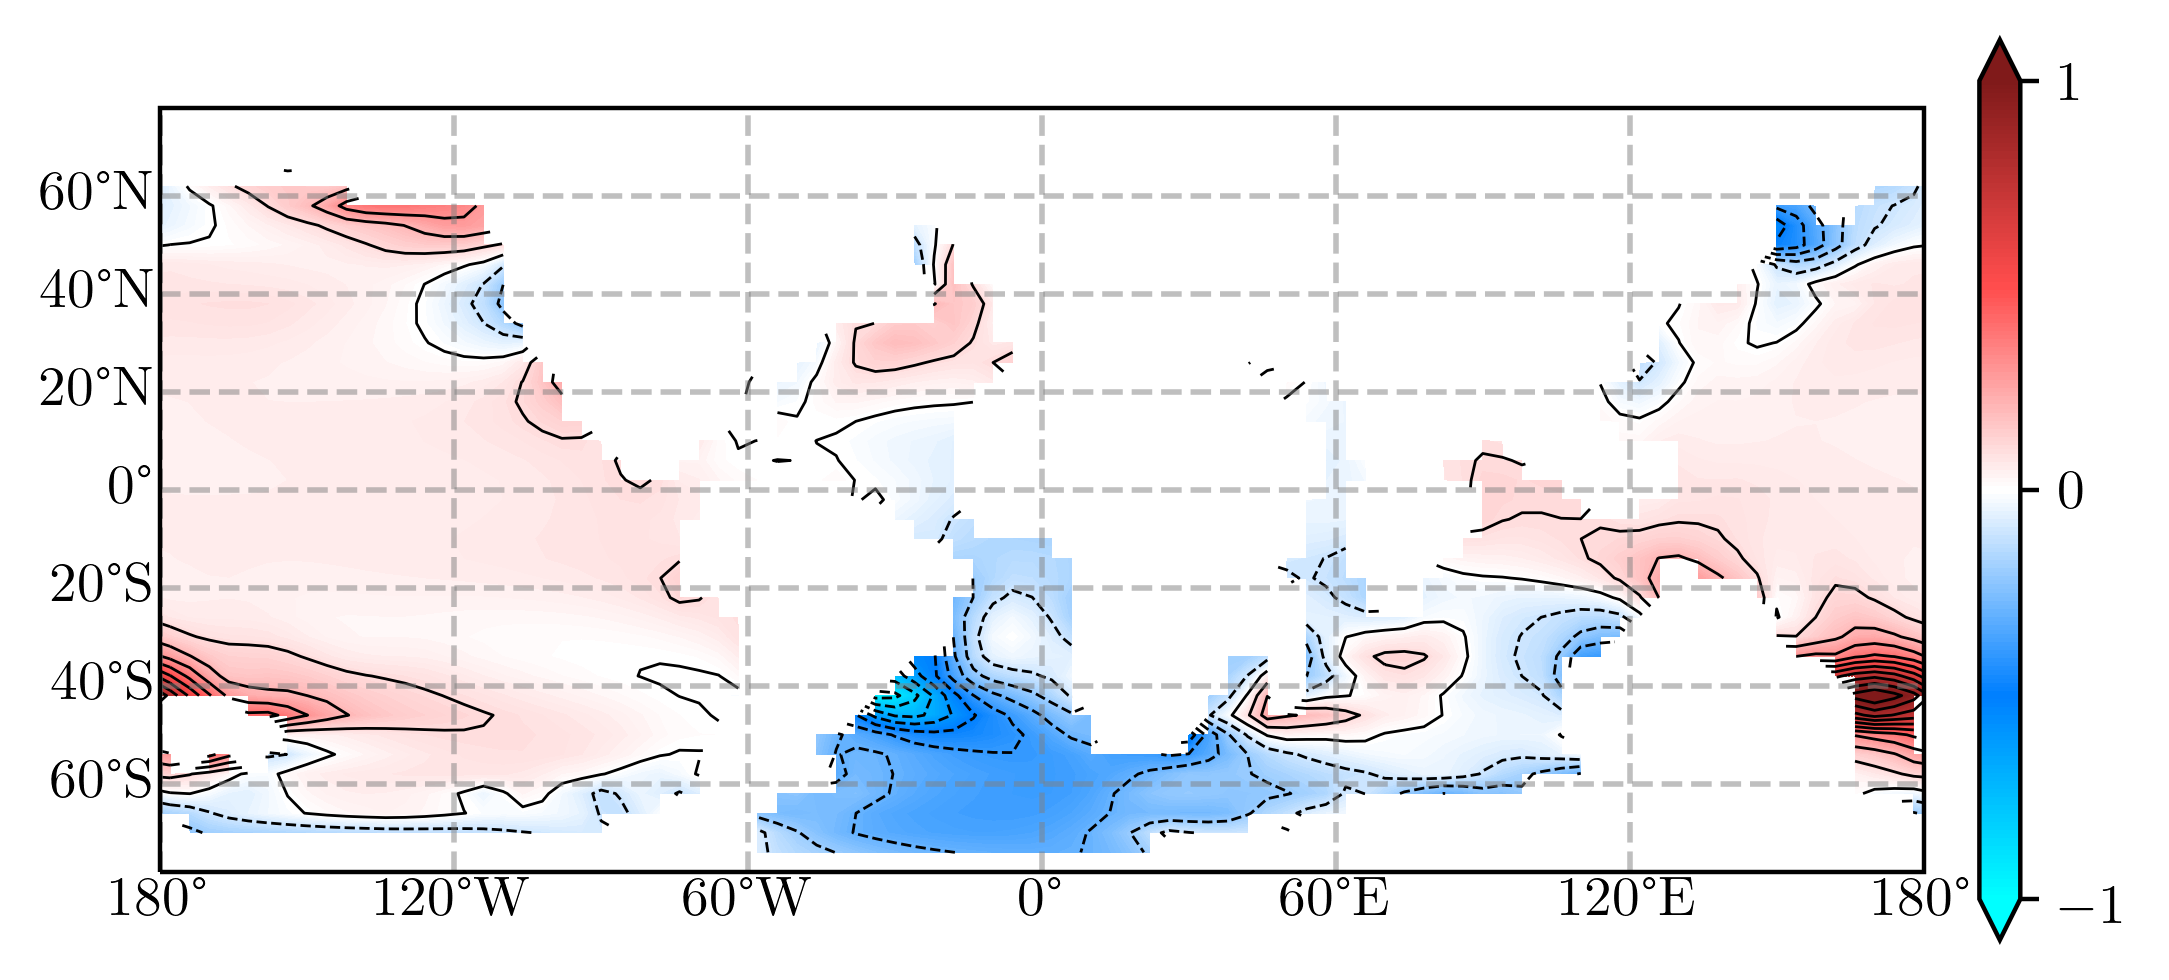
\includegraphics[width=\linewidth]{salt_55_35.png}
		
		
	\end{subfigure}
	\caption{ Comparison between late Paleocene (55Ma) and late Eocene (35Ma) for: \textbf{a)} Temperature ($^{\circ}C$) differences (positive values indicate warming) and  \textbf{b)} Salinity ($psu$) differences (positive values indicate higher salinity)}
\end{figure}

\begin{figure}[H]
	\begin{subfigure}[b]{\linewidth}
		\caption{}
		\label{fig:3520cooling}
		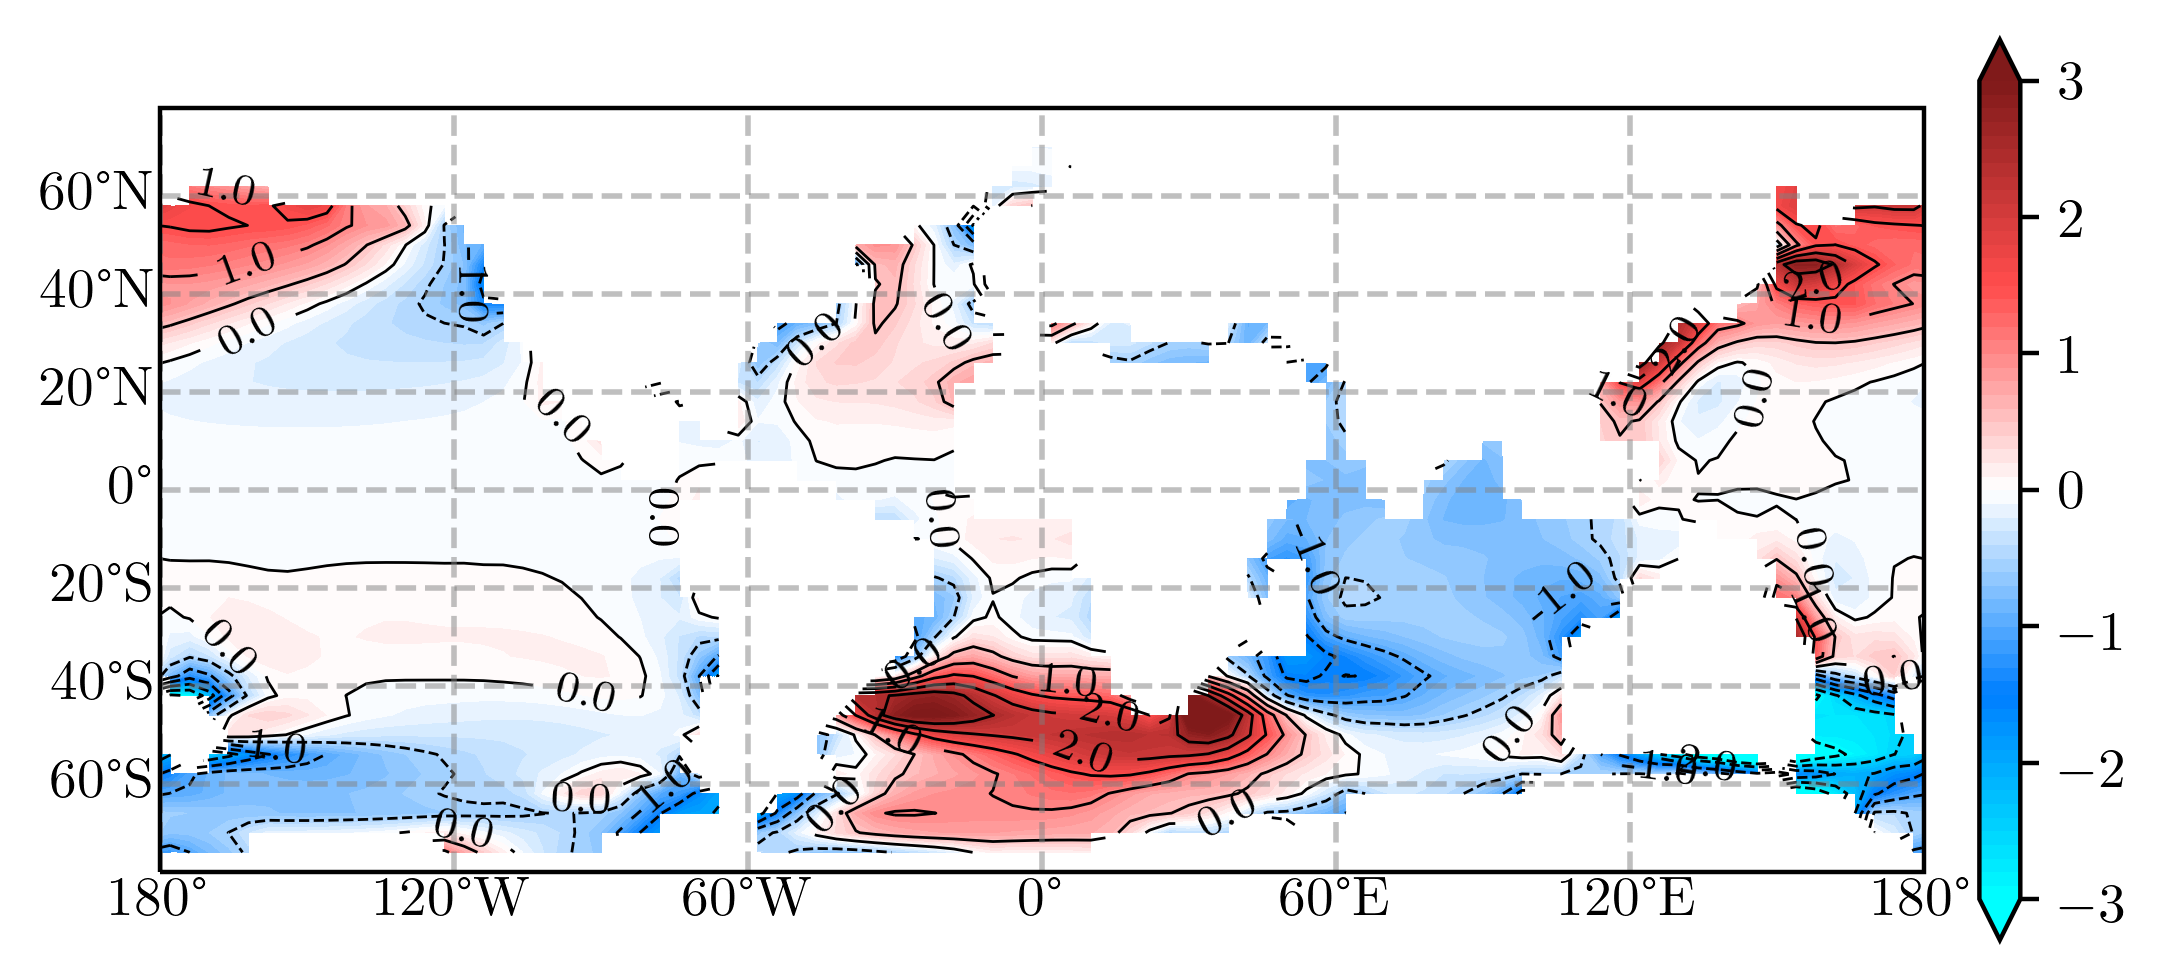
\includegraphics[width=\linewidth]{Paleo_eocene_35_20.png}
		
	\end{subfigure}
	\begin{subfigure}[b]{\linewidth}
		\caption{}
		\label{fig:salt3520cooling}
		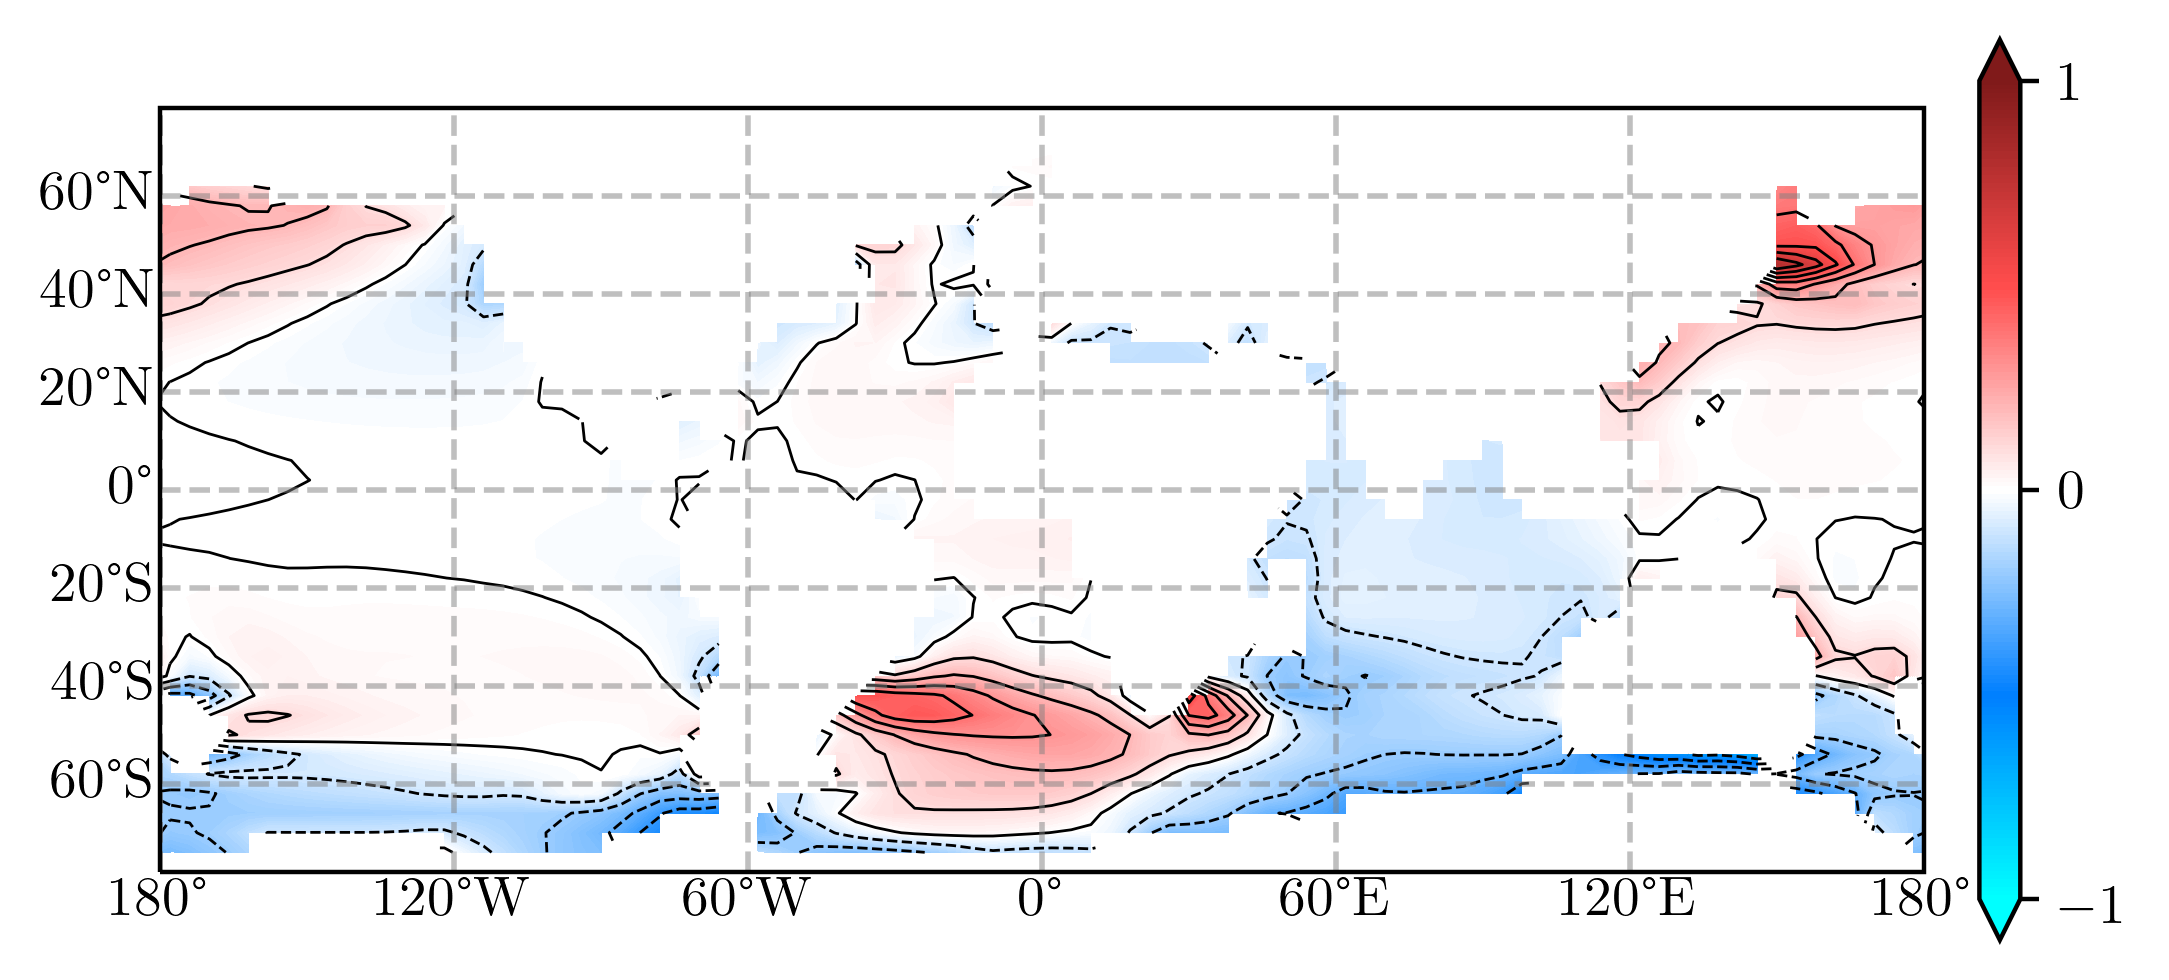
\includegraphics[width=\linewidth]{salt_35_20.png}
		
	\end{subfigure}
	\caption{ Comparison between late Eocene (35Ma) and early Miocene (20Ma) for: \textbf{a)} Temperature ($^{\circ}C$) differences (positive values indicate warming) and  \textbf{b)} Salinity ($psu$) differences (positive values indicate higher salinity)}
\end{figure}

\begin{figure}[H]
	\begin{subfigure}[b]{\linewidth}
		\caption{}
		\label{fig:2010cooling}
		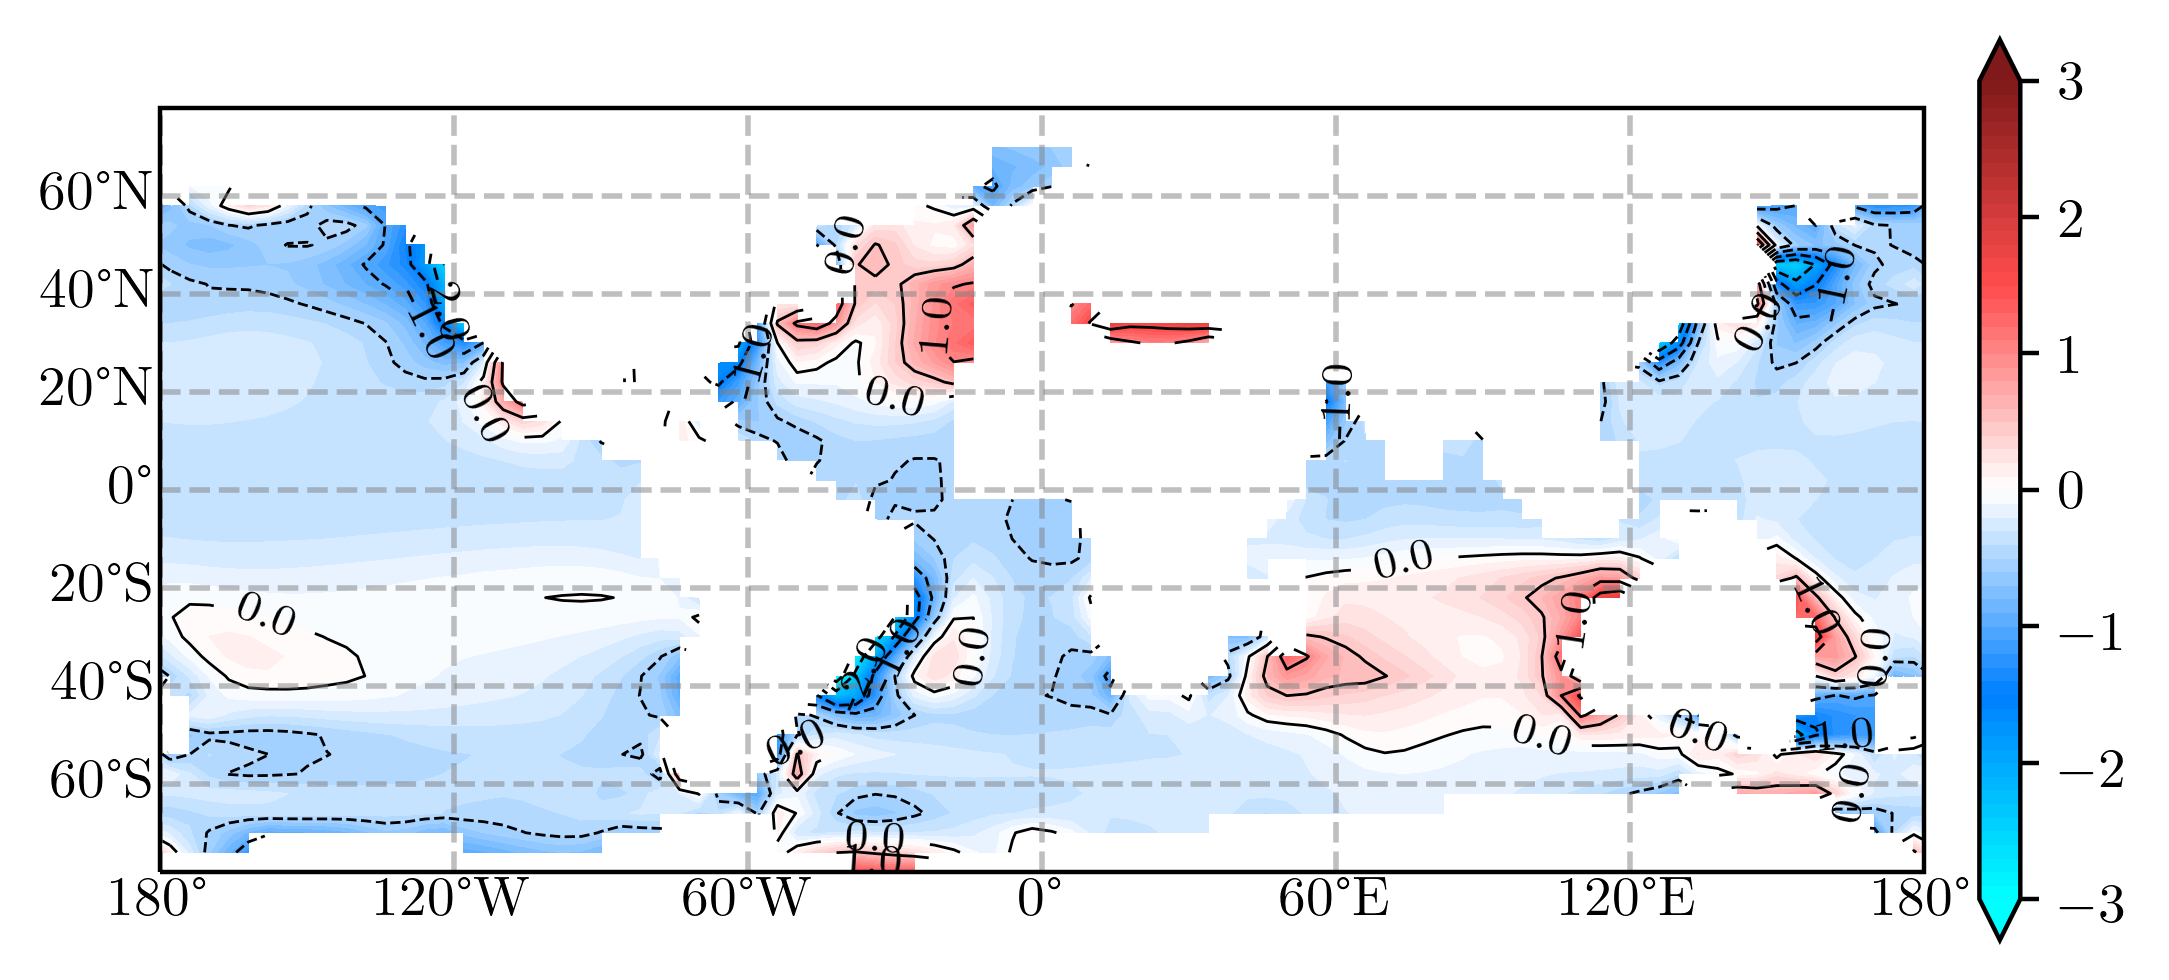
\includegraphics[width=\linewidth]{Paleo_eocene_20_10.png}
	\end{subfigure}
	\begin{subfigure}[b]{\linewidth}
		\caption{}
		\label{fig:salt2010cooling}
		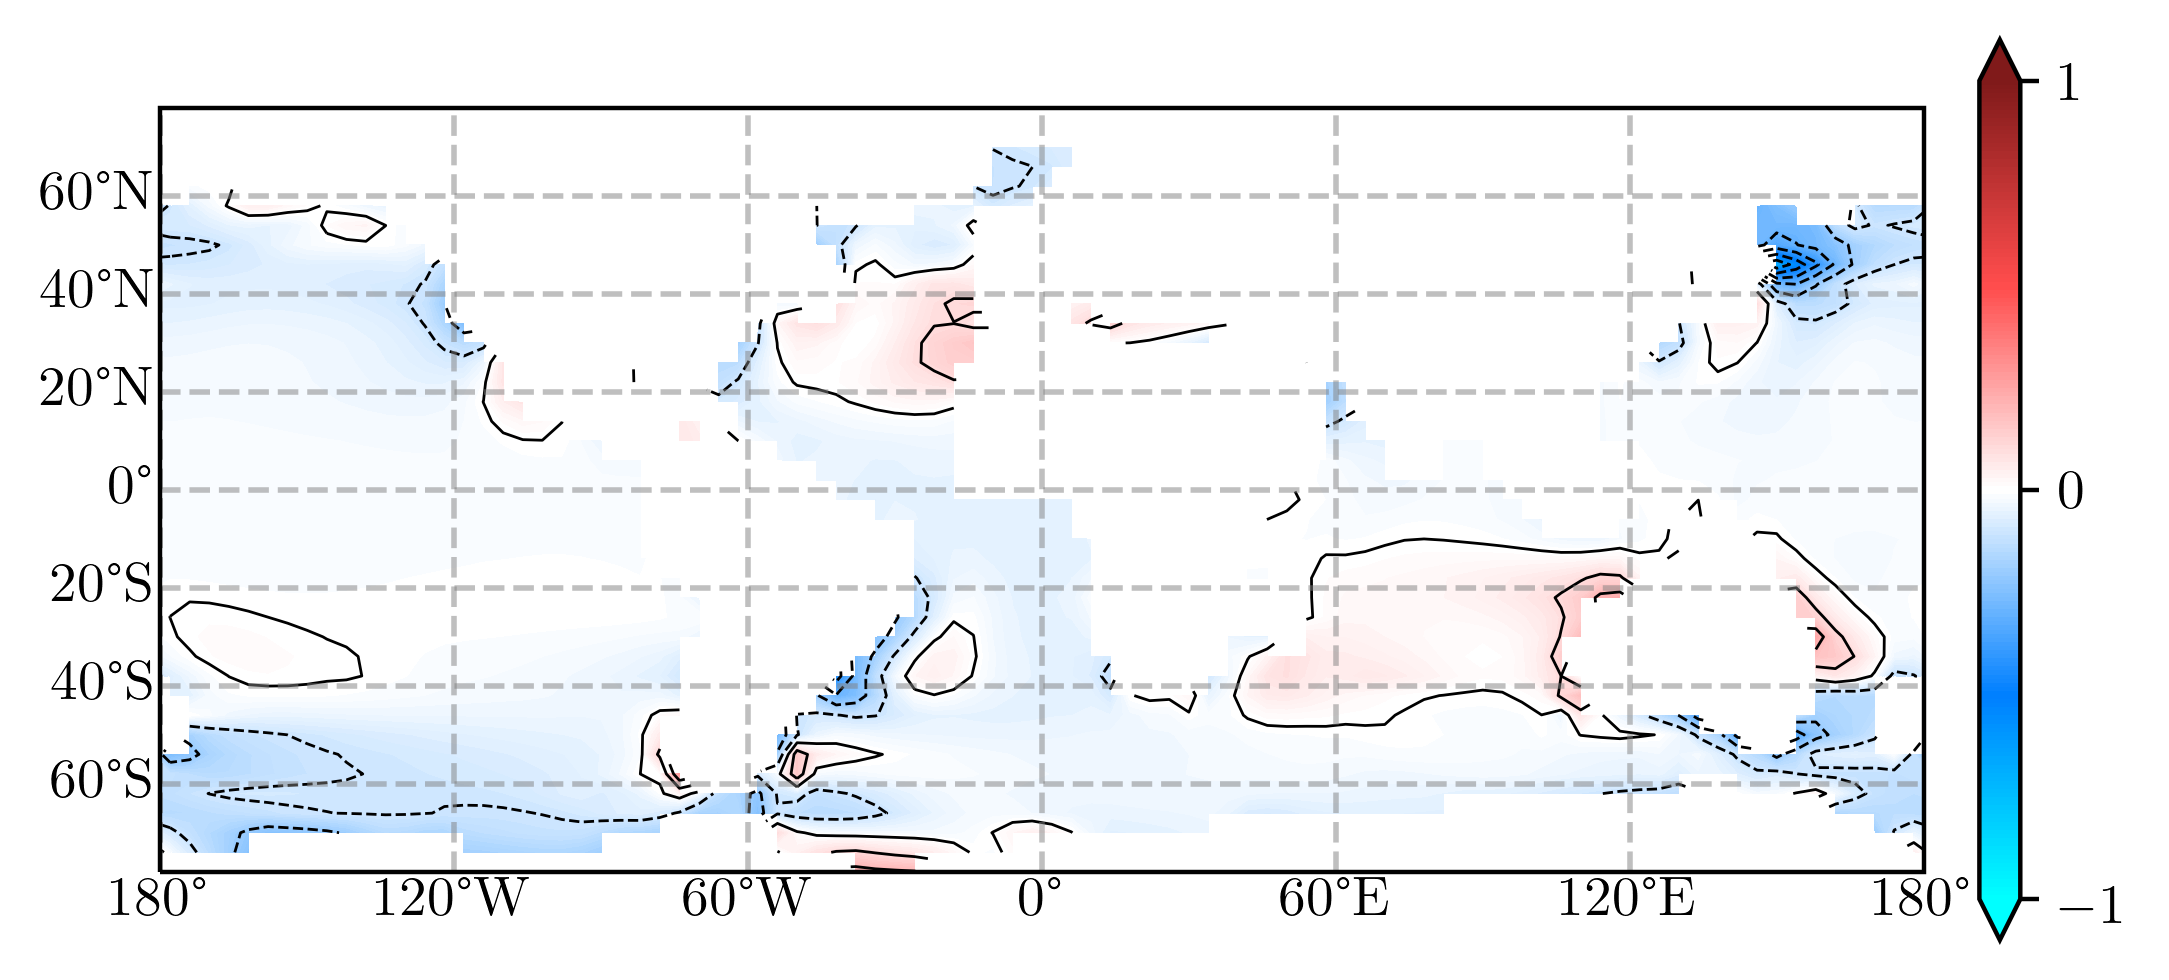
\includegraphics[width=\linewidth]{salt_20_10.png}
	\end{subfigure}
	\caption{ Comparison between early Miocene (20Ma) and late Miocene (10Ma) for: \textbf{a)} Temperature ($^{\circ}C$) differences (positive values indicate warming) and  \textbf{b)} Salinity ($psu$) differences (positive values indicate higher salinity)}
\end{figure}





\section{Summary}
In this paper we have presented a simplified approach to the modeling of past climate systems using Veros. This paper focused heavily on simplified forcings of the global oceanic basins. This allows us  to efficiently look at the effect of changes in geometry on the major oceanic flows. The results shown here are of relatively low resolution and highly idealized boundary conditions. But they still manage to capture some of the features of more complex coupled models for the same time period. The integrations were done on a consumer computer showing that it is now possible to do big ocean simulation research on readily available hardware.

We find a large 
\section{Discussion}

Discuss the results and flaws in these.

Discuss possible future research.

Discuss possible improvements.

Discuss possible 2 degree models.

Discuss troubles with the ACC strength due to the forcings of the current climate.

Discuss the difficulty with trail and error in the model.


\section{Acknowledgments}
This paper would not have been possible without the extensive support of Dr. Anna von der Heydt, who provided valuable input on every single one of the many hurdles that had to be succumbed. I would also like to thank Dr. Michiel Baatsen for providing the bathymetry datasets used in this paper, Prof. Dr. Markus Jochum for providing valuable insight into Veros and Laurits Andreasen for helping with many of our questions and attending our virtual meetings.


%\section{Test images}
%\begin{figure}[H]
%	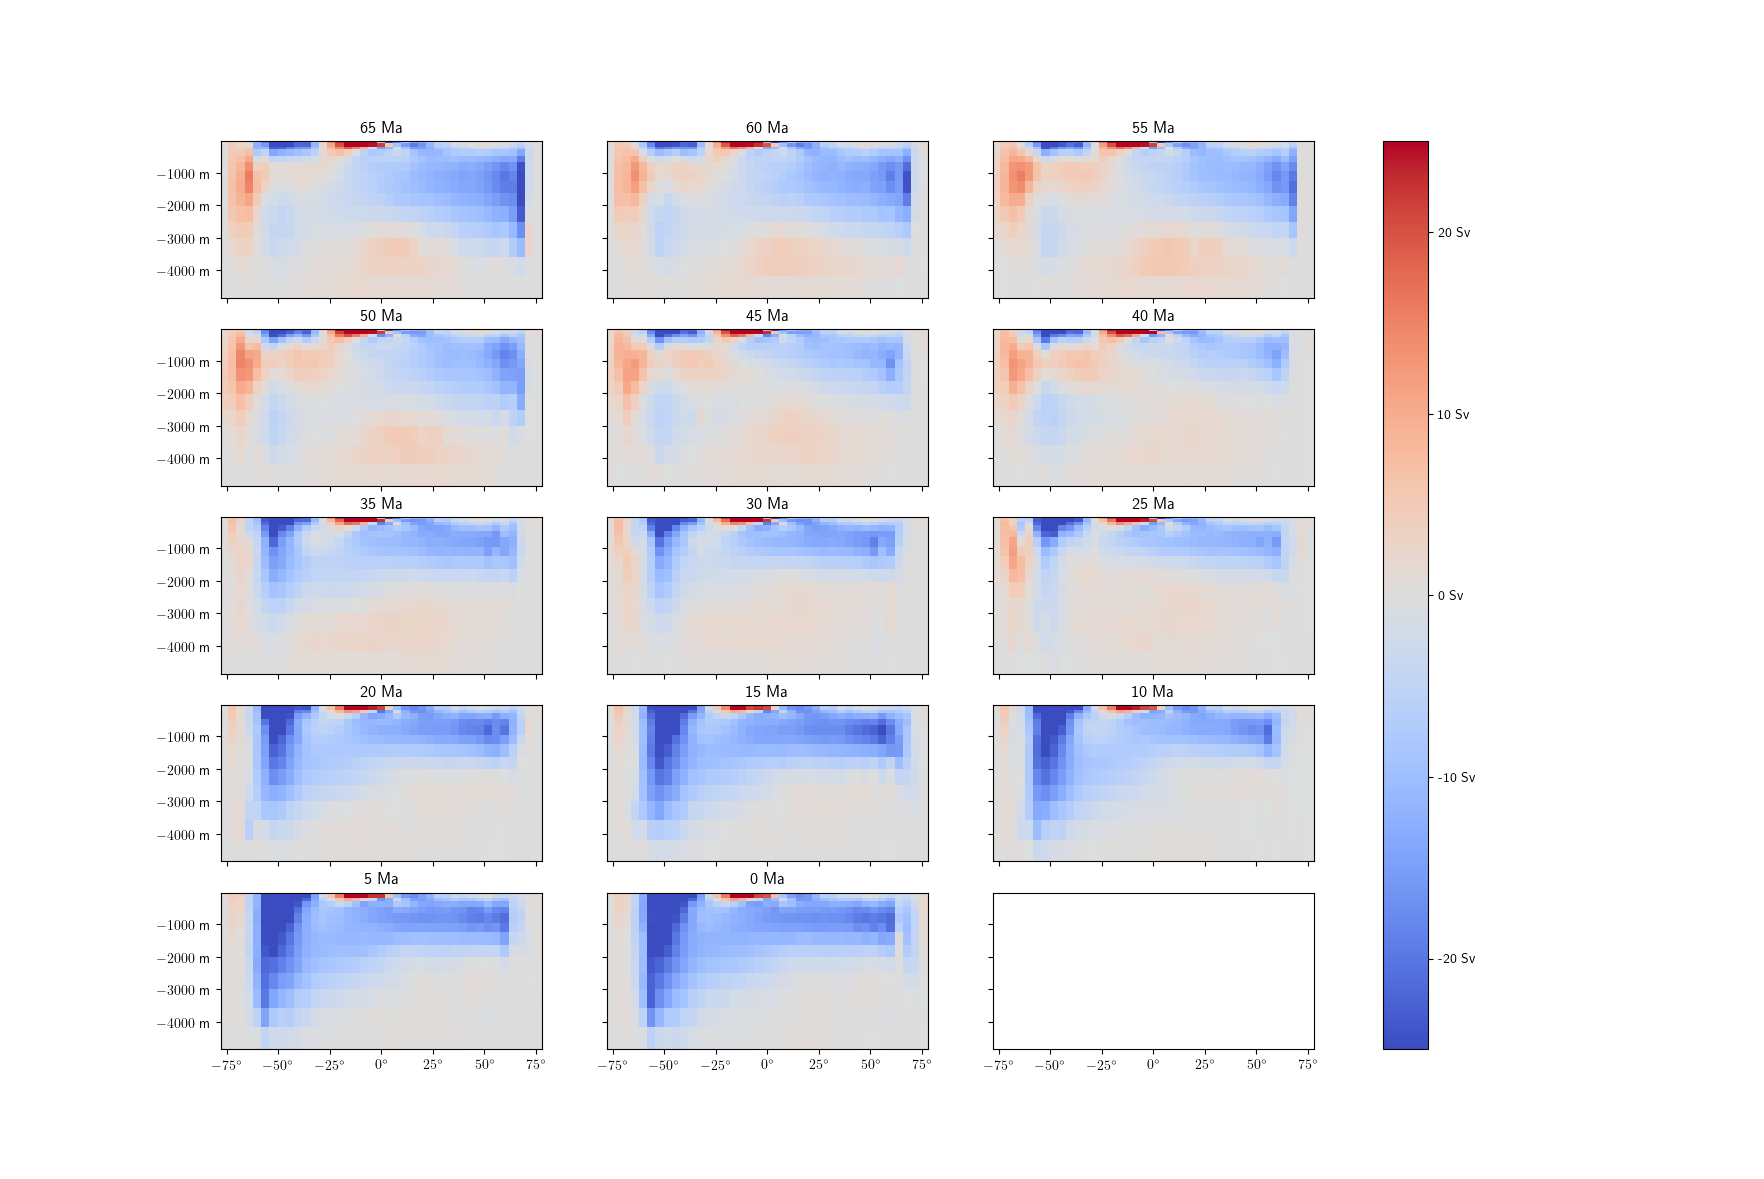
\includegraphics[width=\linewidth]{overturning_overview.png}
%	\caption{test caption}
%	\label{fig:example1}
%\end{figure}
%\end{multicols}
%%example full width overturning
%\begin{figure}[H]
%	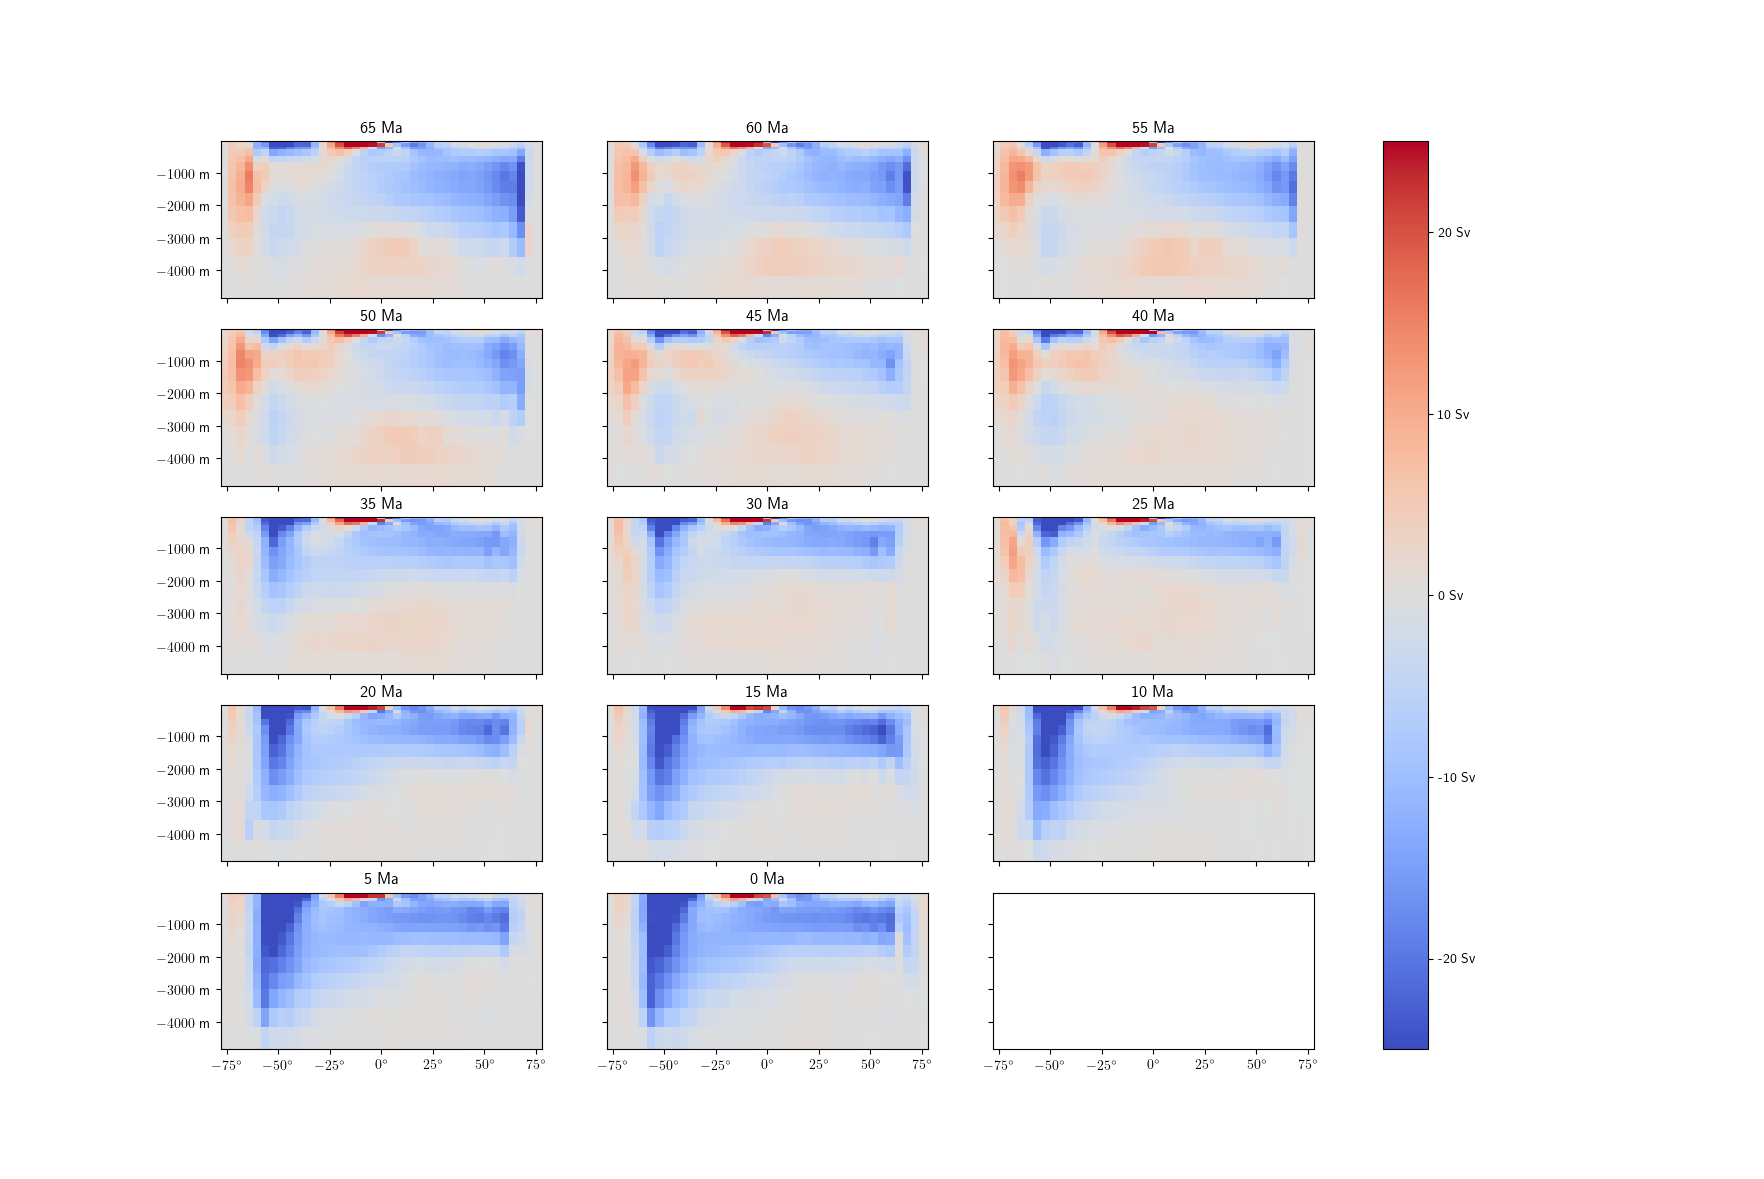
\includegraphics[width=\linewidth]{overturning_overview.png}
%	\caption{test caption}
%	\label{fig:example1}
%\end{figure}
%
%\begin{multicols}{2}

\printbibliography


\end{multicols}
\appendix
\begin{figure}[ht]
		\centering
	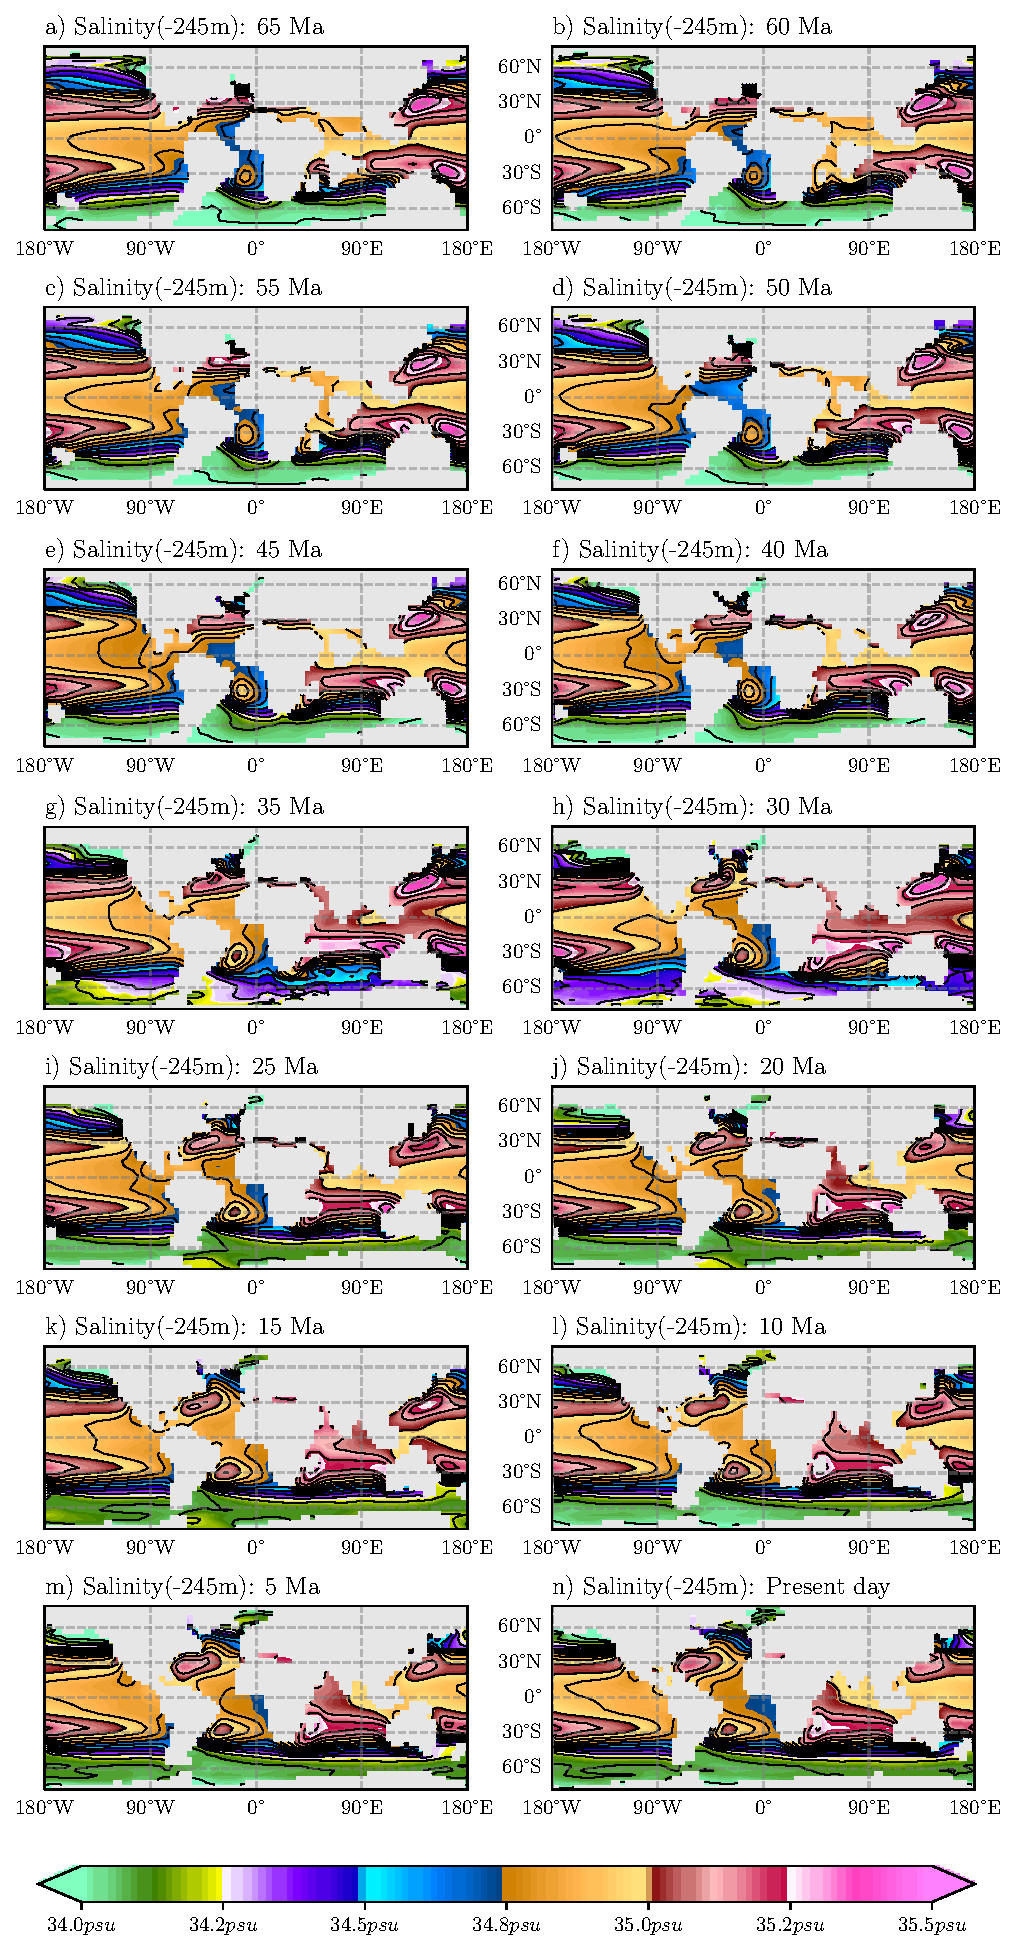
\includegraphics[width=0.7\linewidth]{full_sss.pdf}
	\caption{Salinity at 245m depth for each time step.}
	\label{fig:sss_total}
\end{figure}
\begin{figure}[ht]
	\centering
	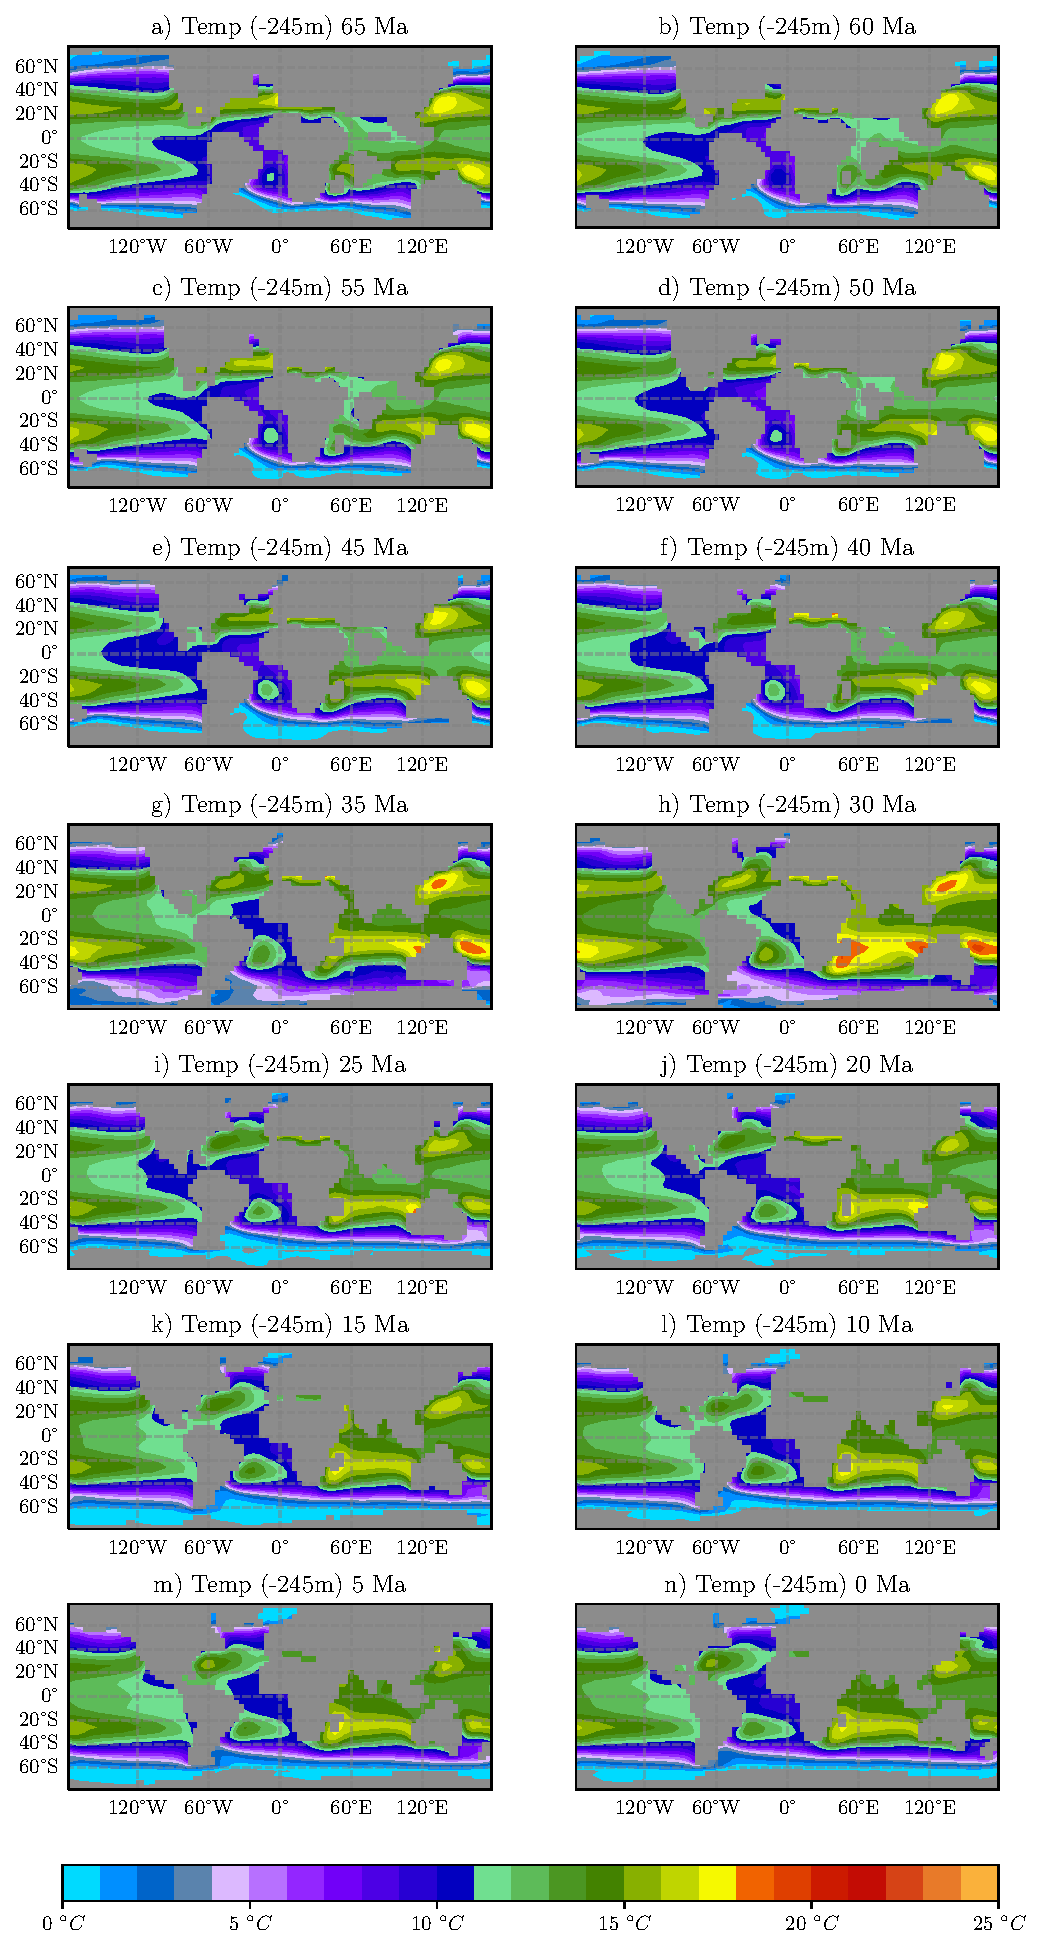
\includegraphics[width=0.7\linewidth]{full_sst.pdf}
	\caption{Temperature at 245m depth for each time step.}
	\label{fig:sst_total}
\end{figure}
\begin{figure}[ht]
	\centering
	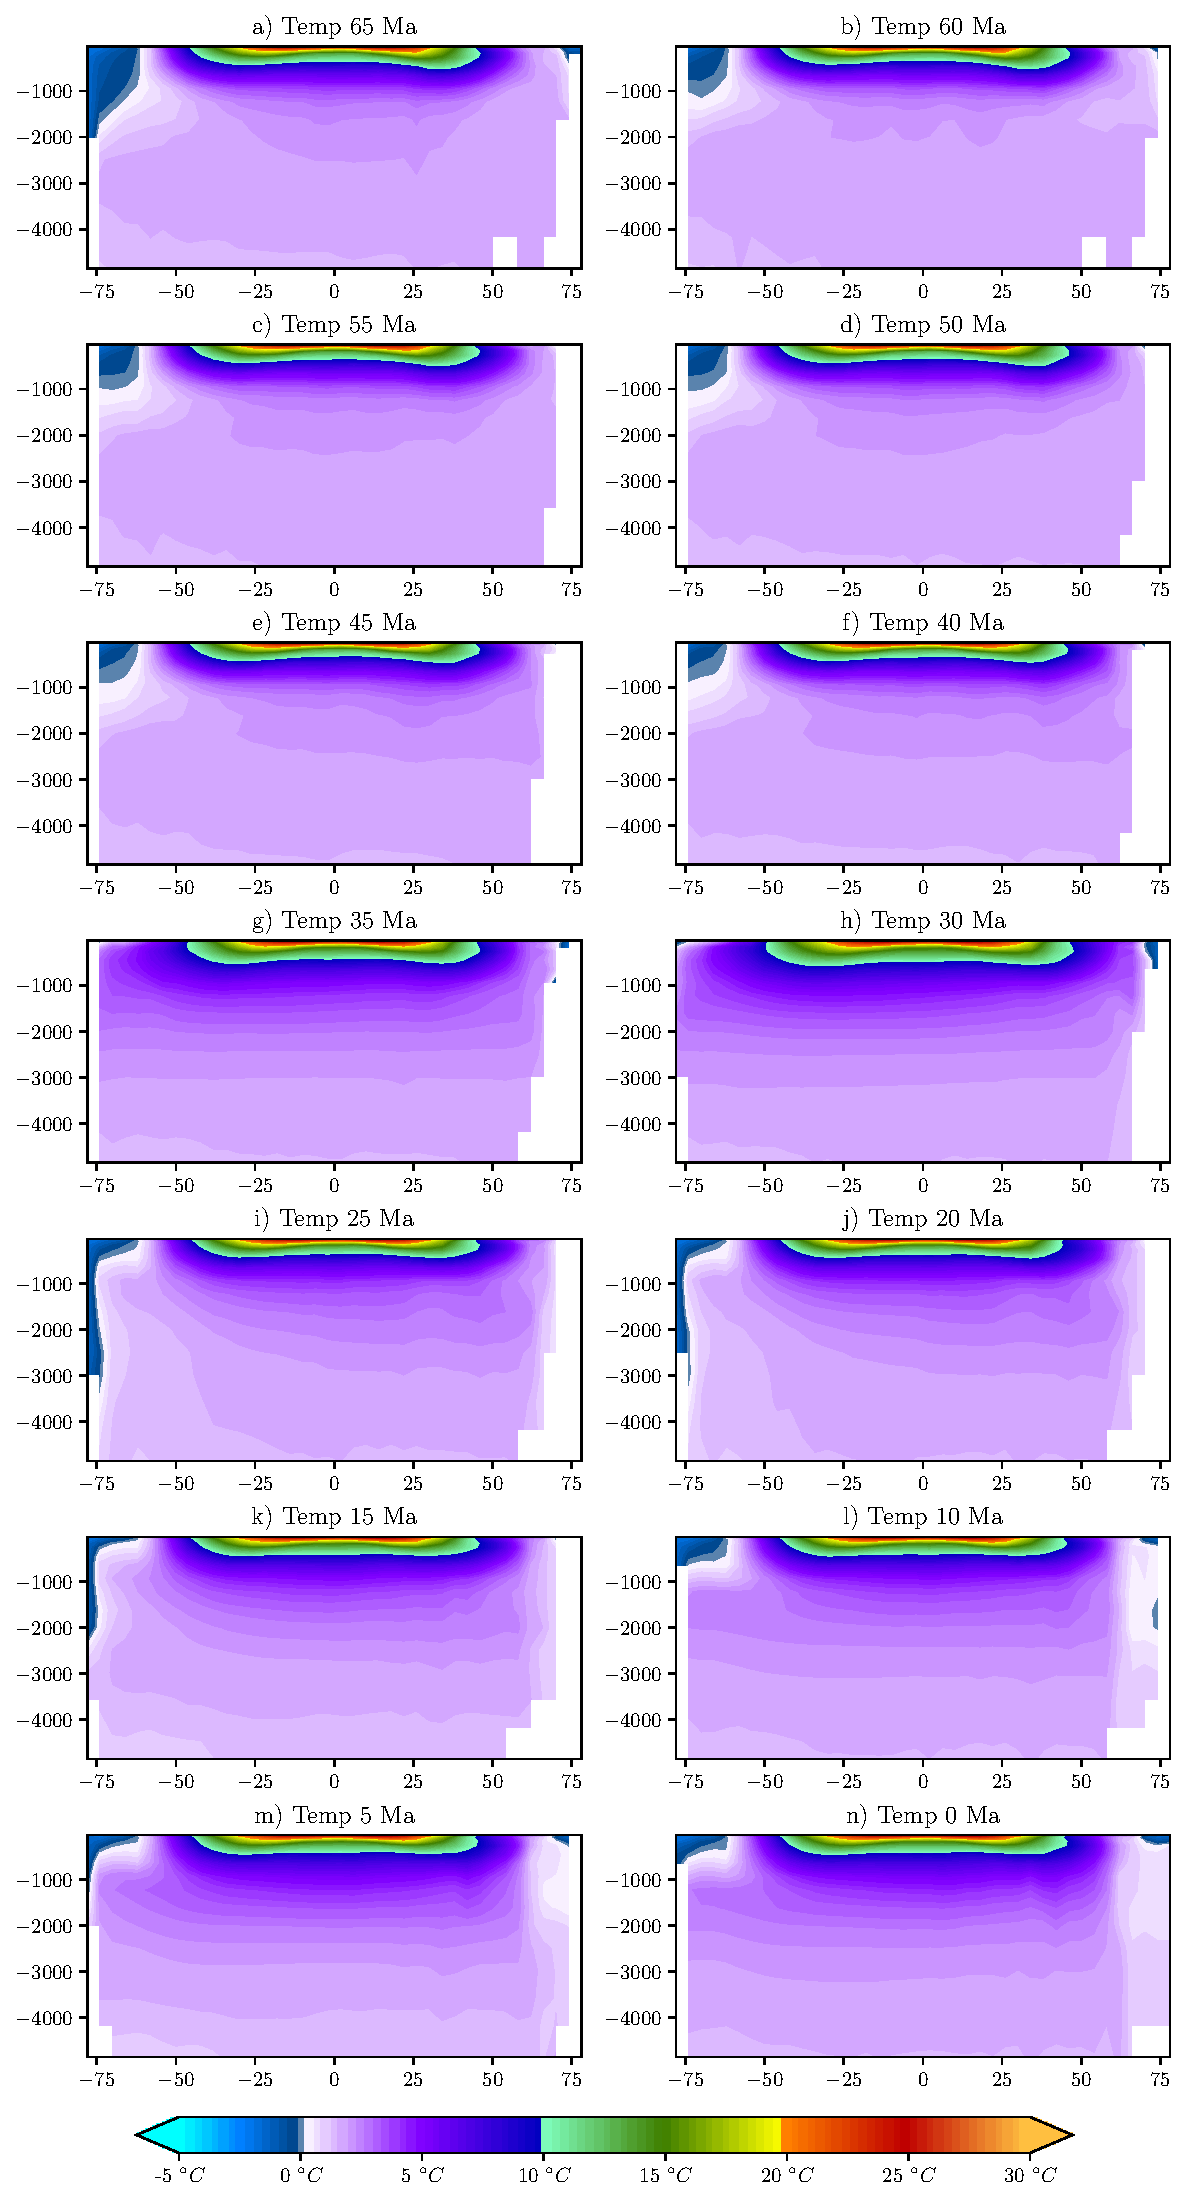
\includegraphics[width=0.7\linewidth]{full_sst_depth.pdf}
	\caption{Latitude depth profile of the zonal mean Temperature}
	\label{fig:sst_zmean_total}
\end{figure}
\begin{figure}[ht]
	\centering
	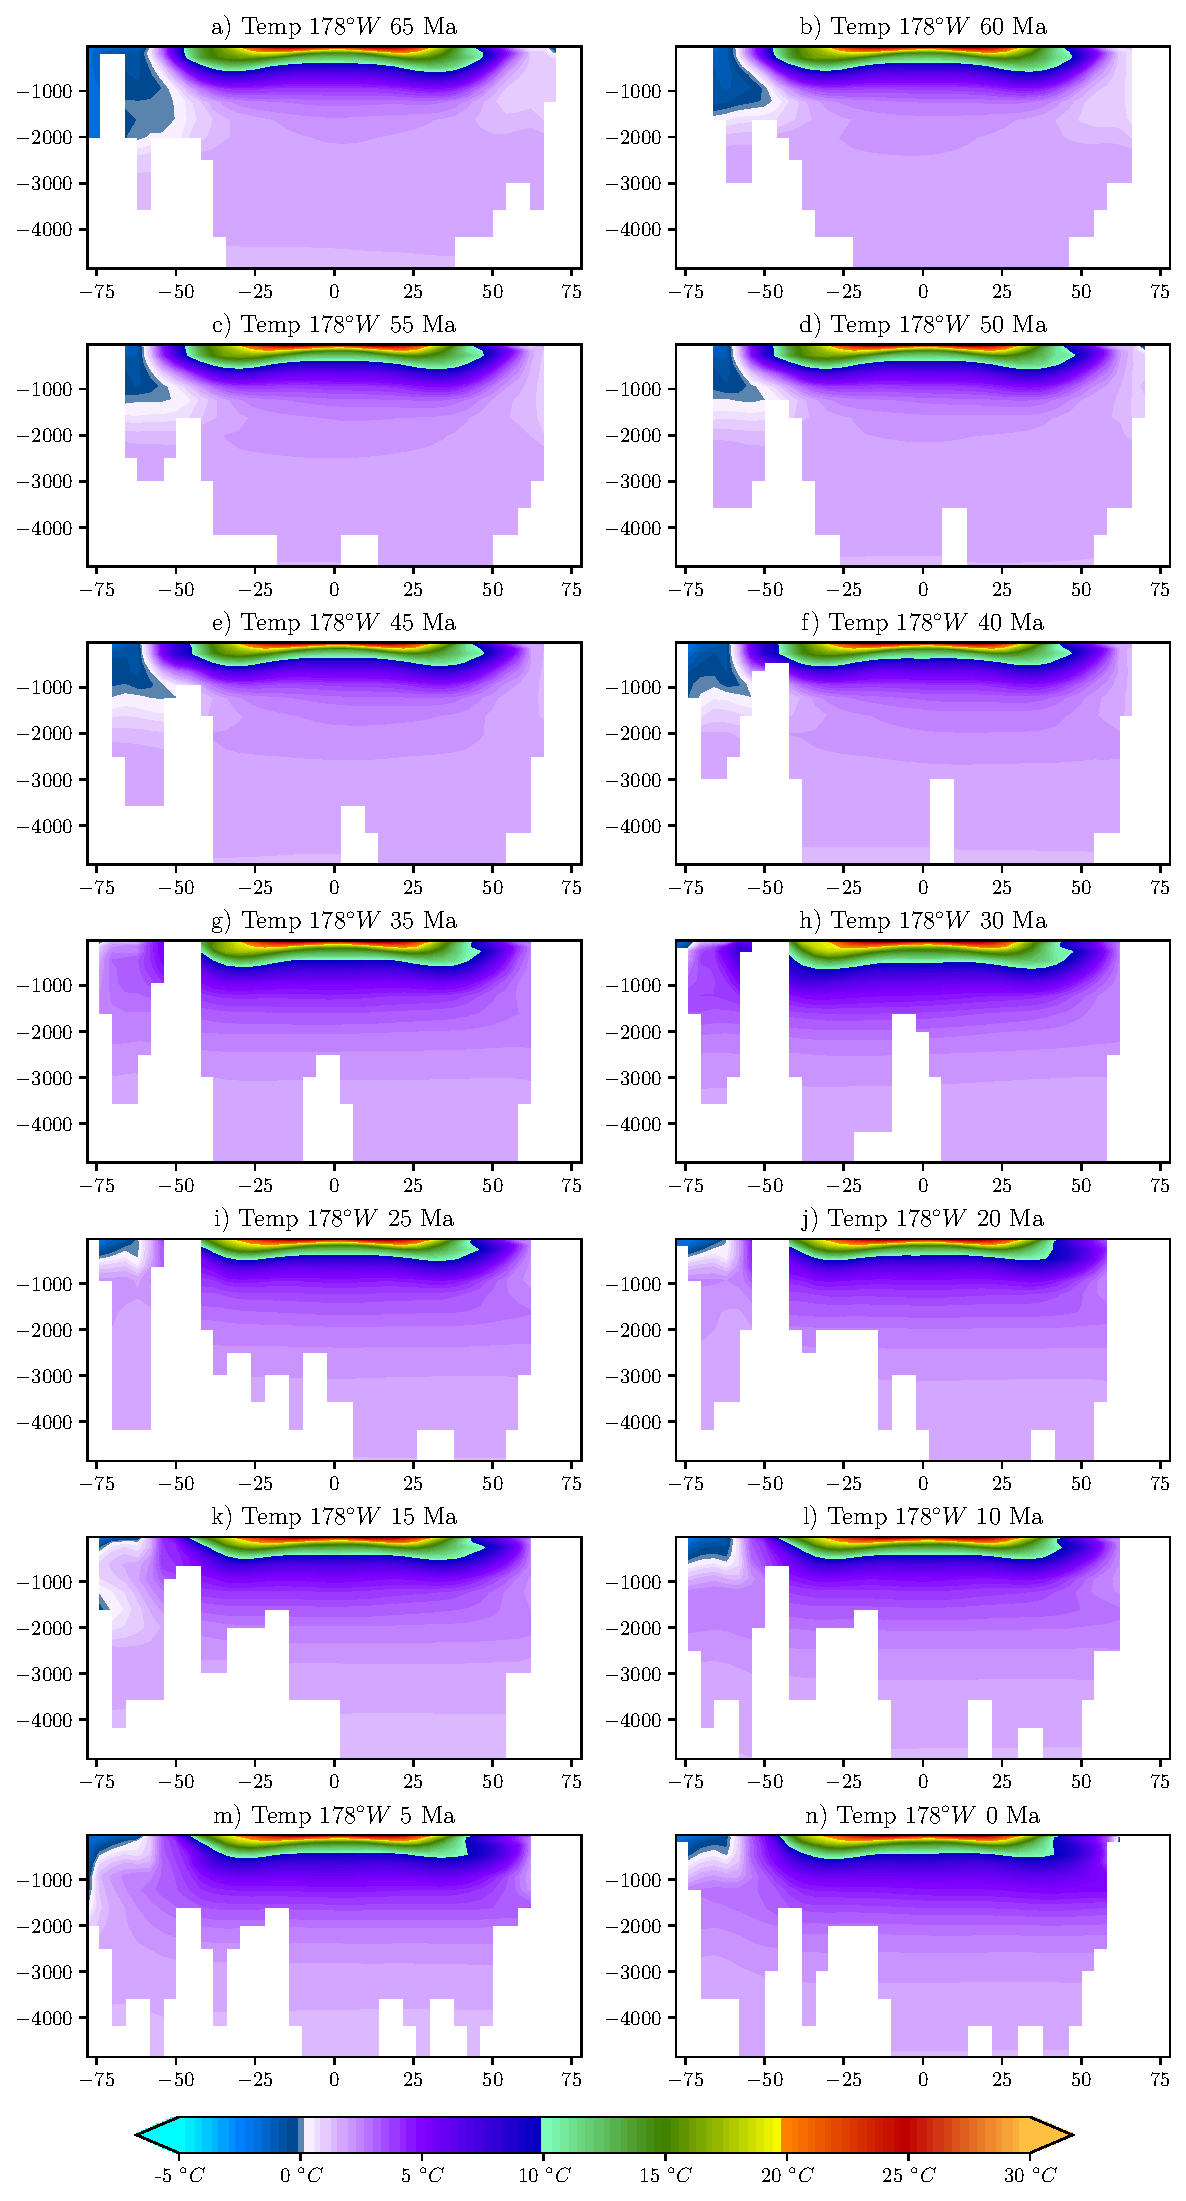
\includegraphics[width=0.7\linewidth]{full_pacific_sst.pdf}
	\caption{Latitude depth profile of the Temperature in the Pacific ($178^{\circ} W$)}
	\label{fig:pacsst_total}
\end{figure}
\begin{figure}[ht]
	\centering
	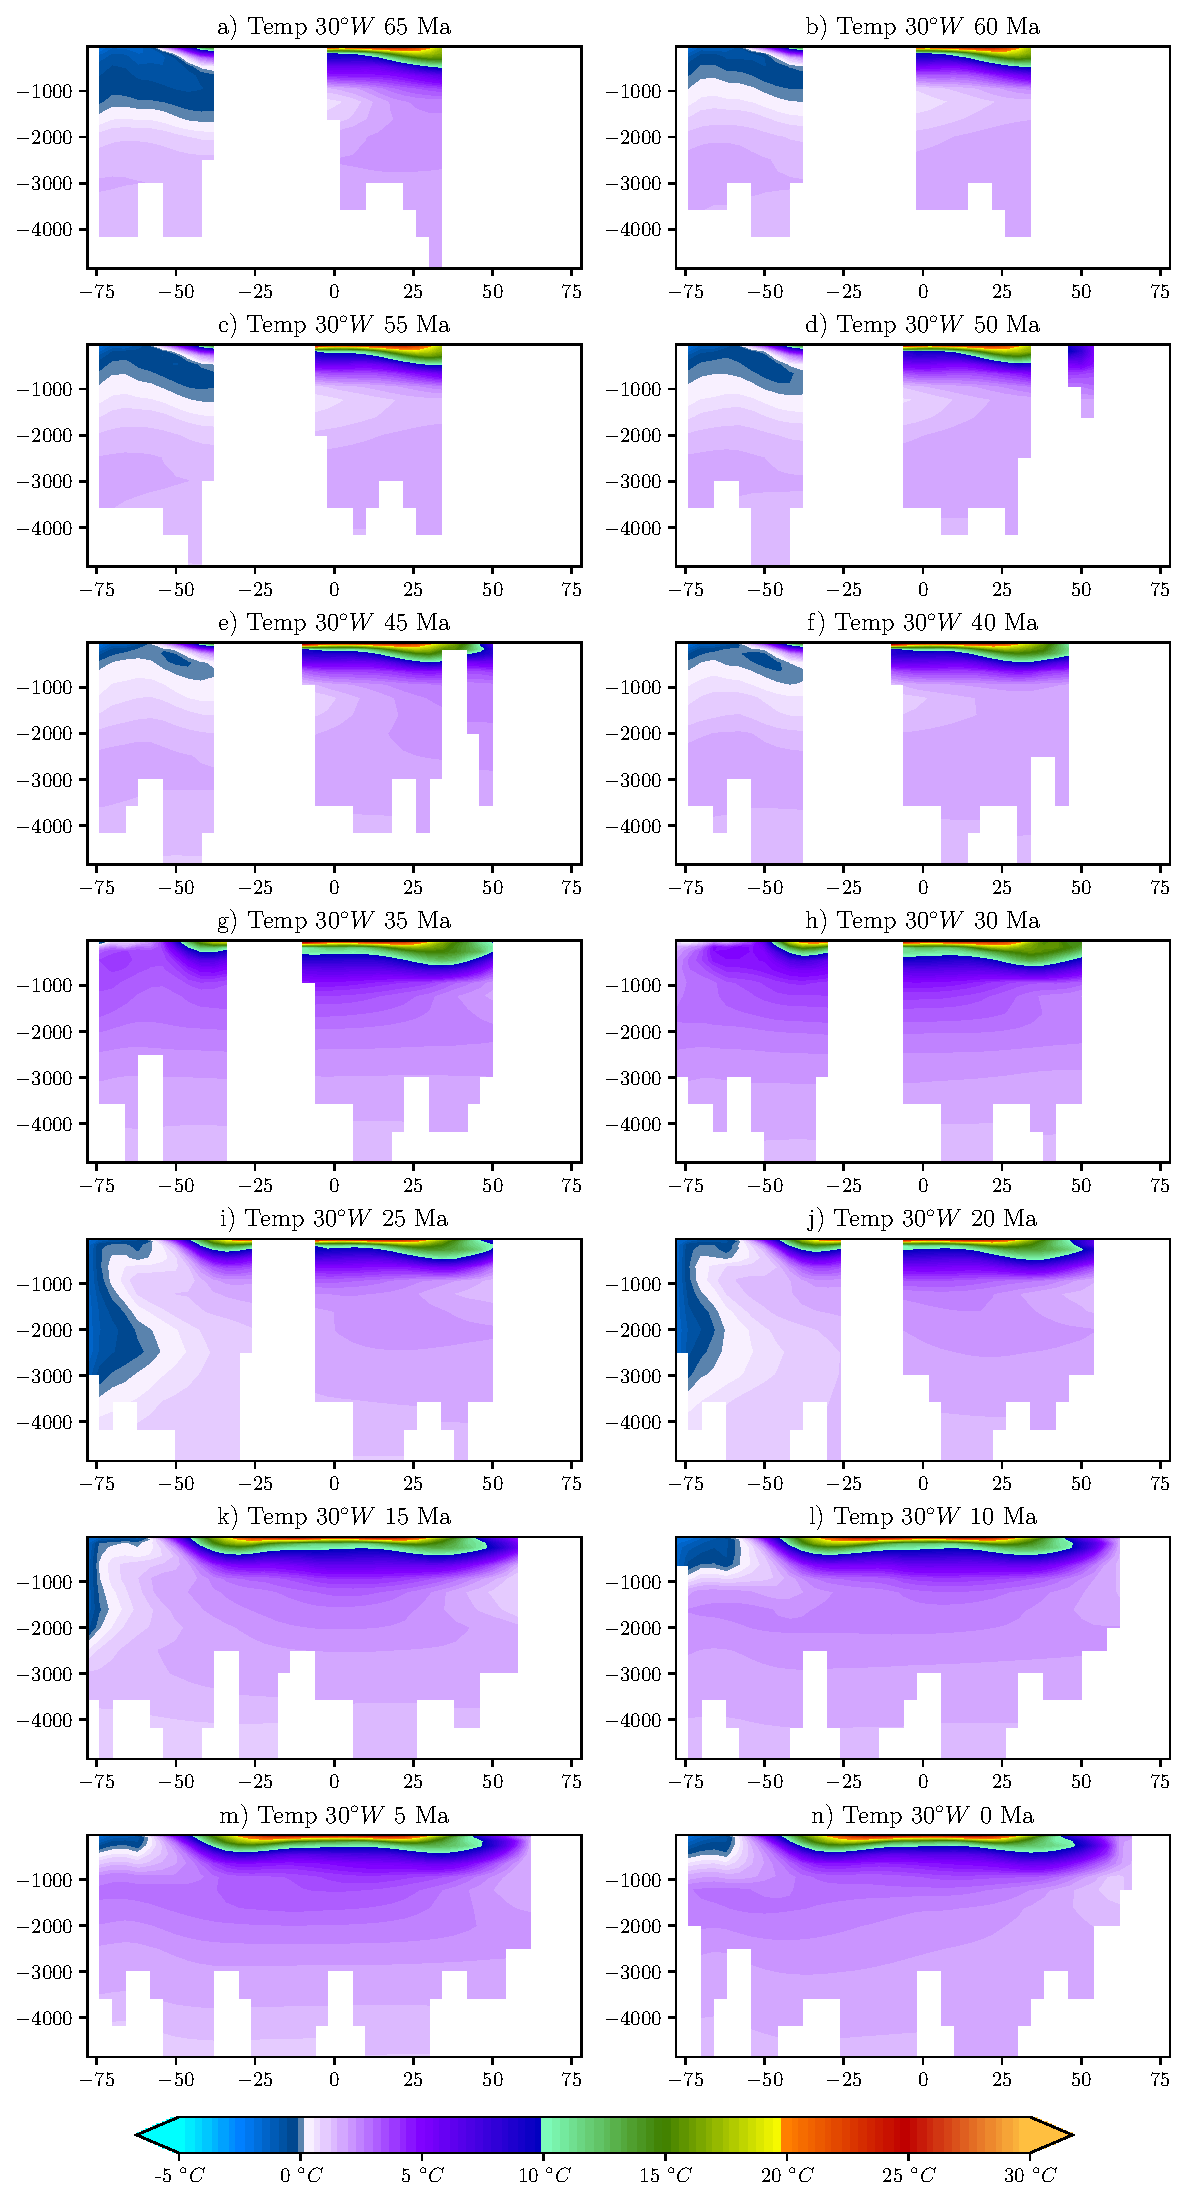
\includegraphics[width=0.7\linewidth]{full_atlantic_sst.pdf}
	\caption{Latitude depth profile of the Temperature in the Atlantic ($178^{\circ} W$)}
	\label{fig:atlsst_total}
\end{figure}
\begin{figure}[ht]
	\centering
	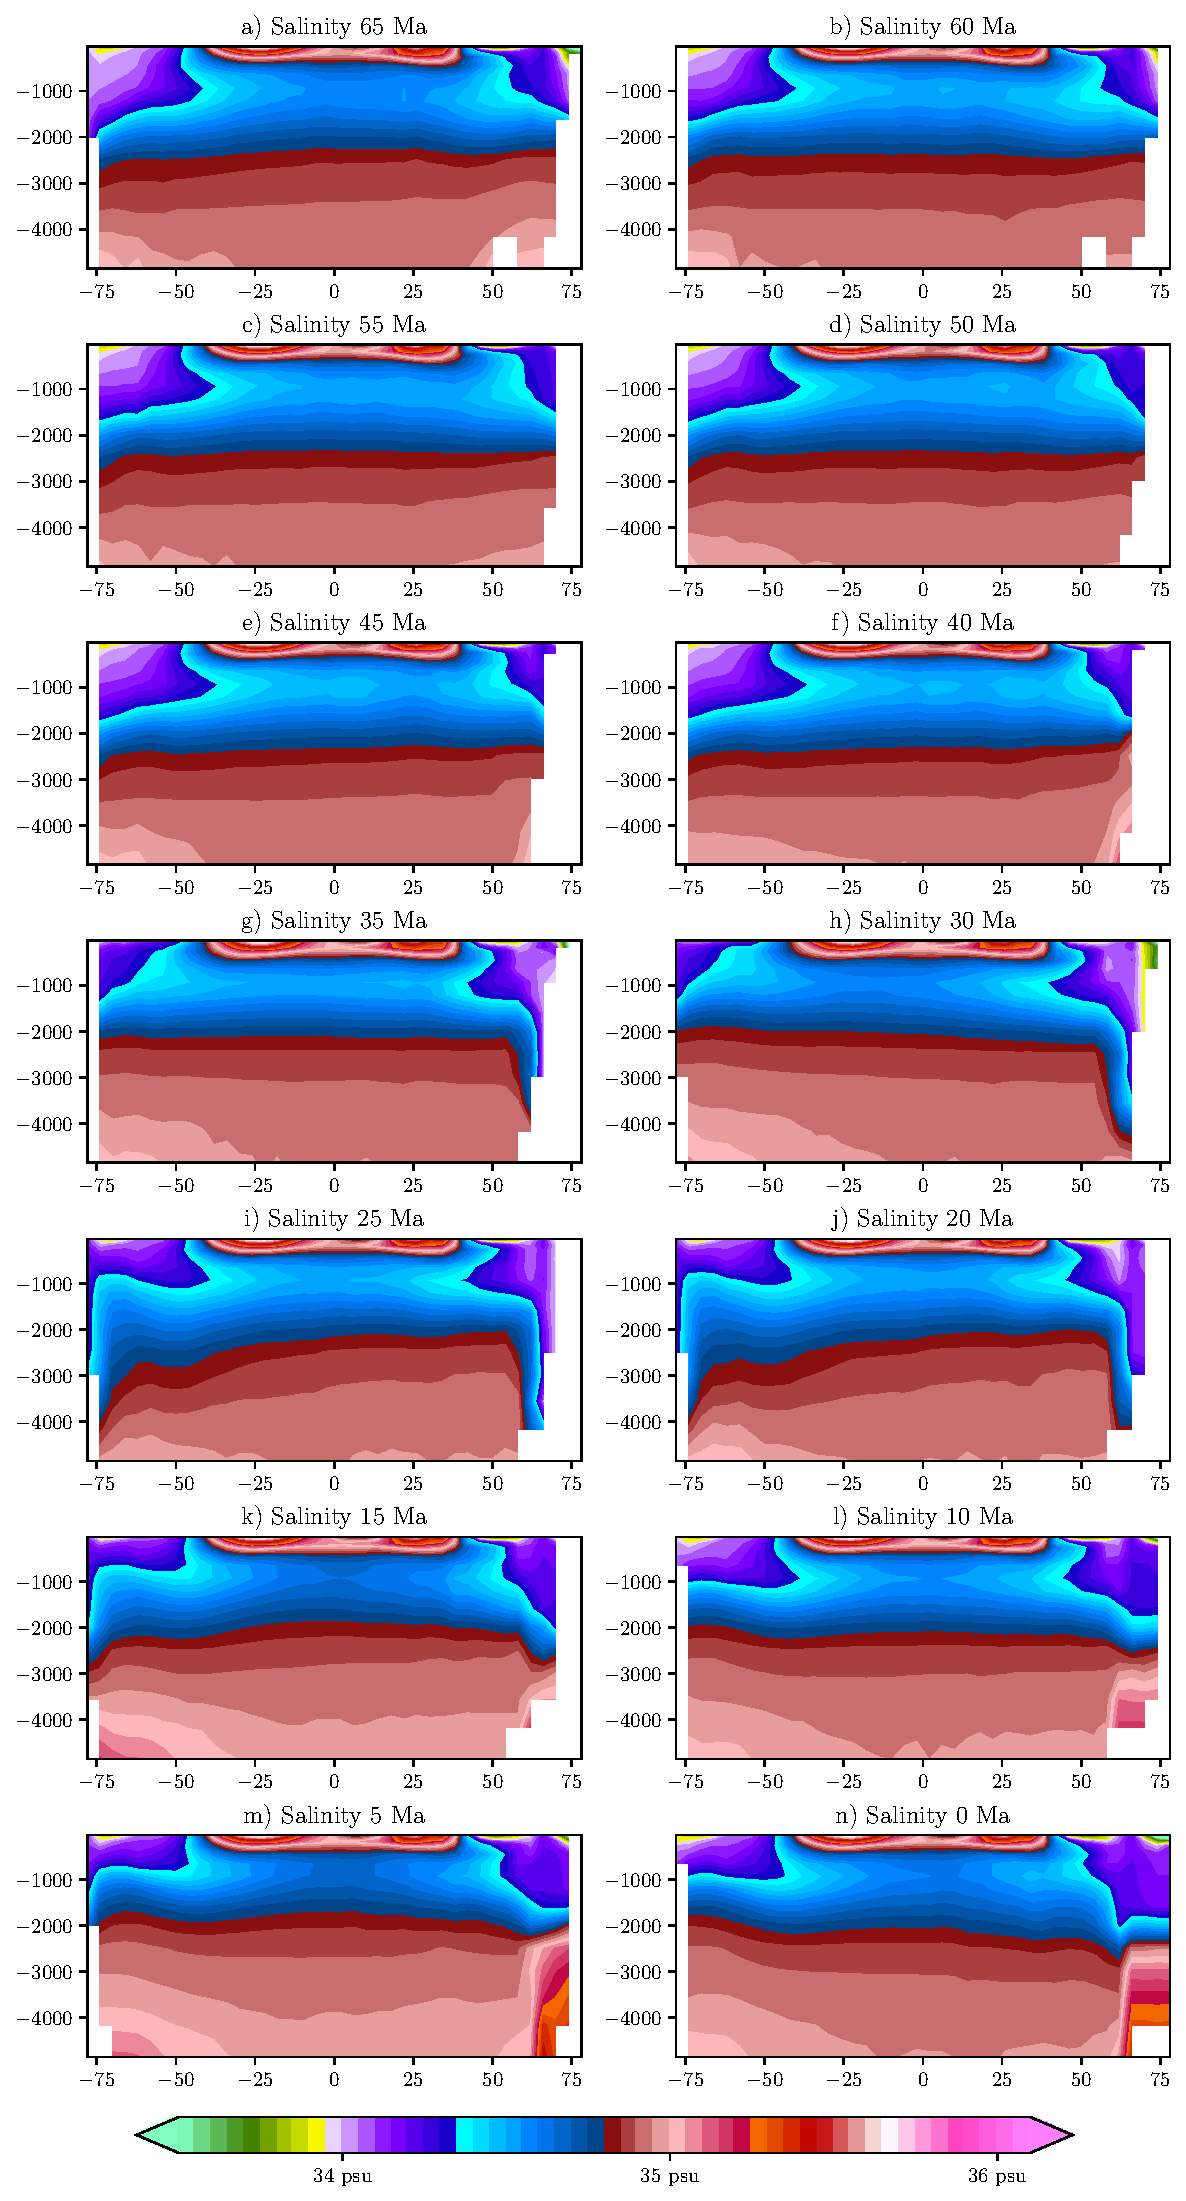
\includegraphics[width=0.7\linewidth]{full_sss_depth.pdf}
	\caption{Latitude depth profile of the zonal mean Salinity}
	\label{fig:atlsst_total}
\end{figure}



\end{document}
